% Options for packages loaded elsewhere
\PassOptionsToPackage{unicode}{hyperref}
\PassOptionsToPackage{hyphens}{url}
\PassOptionsToPackage{dvipsnames,svgnames,x11names}{xcolor}
%
\documentclass[
  letterpaper,
  DIV=11,
  numbers=noendperiod]{scrreprt}

\usepackage{amsmath,amssymb}
\usepackage{iftex}
\ifPDFTeX
  \usepackage[T1]{fontenc}
  \usepackage[utf8]{inputenc}
  \usepackage{textcomp} % provide euro and other symbols
\else % if luatex or xetex
  \usepackage{unicode-math}
  \defaultfontfeatures{Scale=MatchLowercase}
  \defaultfontfeatures[\rmfamily]{Ligatures=TeX,Scale=1}
\fi
\usepackage{lmodern}
\ifPDFTeX\else  
    % xetex/luatex font selection
\fi
% Use upquote if available, for straight quotes in verbatim environments
\IfFileExists{upquote.sty}{\usepackage{upquote}}{}
\IfFileExists{microtype.sty}{% use microtype if available
  \usepackage[]{microtype}
  \UseMicrotypeSet[protrusion]{basicmath} % disable protrusion for tt fonts
}{}
\makeatletter
\@ifundefined{KOMAClassName}{% if non-KOMA class
  \IfFileExists{parskip.sty}{%
    \usepackage{parskip}
  }{% else
    \setlength{\parindent}{0pt}
    \setlength{\parskip}{6pt plus 2pt minus 1pt}}
}{% if KOMA class
  \KOMAoptions{parskip=half}}
\makeatother
\usepackage{xcolor}
\setlength{\emergencystretch}{3em} % prevent overfull lines
\setcounter{secnumdepth}{2}
% Make \paragraph and \subparagraph free-standing
\ifx\paragraph\undefined\else
  \let\oldparagraph\paragraph
  \renewcommand{\paragraph}[1]{\oldparagraph{#1}\mbox{}}
\fi
\ifx\subparagraph\undefined\else
  \let\oldsubparagraph\subparagraph
  \renewcommand{\subparagraph}[1]{\oldsubparagraph{#1}\mbox{}}
\fi

\usepackage{color}
\usepackage{fancyvrb}
\newcommand{\VerbBar}{|}
\newcommand{\VERB}{\Verb[commandchars=\\\{\}]}
\DefineVerbatimEnvironment{Highlighting}{Verbatim}{commandchars=\\\{\}}
% Add ',fontsize=\small' for more characters per line
\usepackage{framed}
\definecolor{shadecolor}{RGB}{241,243,245}
\newenvironment{Shaded}{\begin{snugshade}}{\end{snugshade}}
\newcommand{\AlertTok}[1]{\textcolor[rgb]{0.68,0.00,0.00}{#1}}
\newcommand{\AnnotationTok}[1]{\textcolor[rgb]{0.37,0.37,0.37}{#1}}
\newcommand{\AttributeTok}[1]{\textcolor[rgb]{0.40,0.45,0.13}{#1}}
\newcommand{\BaseNTok}[1]{\textcolor[rgb]{0.68,0.00,0.00}{#1}}
\newcommand{\BuiltInTok}[1]{\textcolor[rgb]{0.00,0.23,0.31}{#1}}
\newcommand{\CharTok}[1]{\textcolor[rgb]{0.13,0.47,0.30}{#1}}
\newcommand{\CommentTok}[1]{\textcolor[rgb]{0.37,0.37,0.37}{#1}}
\newcommand{\CommentVarTok}[1]{\textcolor[rgb]{0.37,0.37,0.37}{\textit{#1}}}
\newcommand{\ConstantTok}[1]{\textcolor[rgb]{0.56,0.35,0.01}{#1}}
\newcommand{\ControlFlowTok}[1]{\textcolor[rgb]{0.00,0.23,0.31}{#1}}
\newcommand{\DataTypeTok}[1]{\textcolor[rgb]{0.68,0.00,0.00}{#1}}
\newcommand{\DecValTok}[1]{\textcolor[rgb]{0.68,0.00,0.00}{#1}}
\newcommand{\DocumentationTok}[1]{\textcolor[rgb]{0.37,0.37,0.37}{\textit{#1}}}
\newcommand{\ErrorTok}[1]{\textcolor[rgb]{0.68,0.00,0.00}{#1}}
\newcommand{\ExtensionTok}[1]{\textcolor[rgb]{0.00,0.23,0.31}{#1}}
\newcommand{\FloatTok}[1]{\textcolor[rgb]{0.68,0.00,0.00}{#1}}
\newcommand{\FunctionTok}[1]{\textcolor[rgb]{0.28,0.35,0.67}{#1}}
\newcommand{\ImportTok}[1]{\textcolor[rgb]{0.00,0.46,0.62}{#1}}
\newcommand{\InformationTok}[1]{\textcolor[rgb]{0.37,0.37,0.37}{#1}}
\newcommand{\KeywordTok}[1]{\textcolor[rgb]{0.00,0.23,0.31}{#1}}
\newcommand{\NormalTok}[1]{\textcolor[rgb]{0.00,0.23,0.31}{#1}}
\newcommand{\OperatorTok}[1]{\textcolor[rgb]{0.37,0.37,0.37}{#1}}
\newcommand{\OtherTok}[1]{\textcolor[rgb]{0.00,0.23,0.31}{#1}}
\newcommand{\PreprocessorTok}[1]{\textcolor[rgb]{0.68,0.00,0.00}{#1}}
\newcommand{\RegionMarkerTok}[1]{\textcolor[rgb]{0.00,0.23,0.31}{#1}}
\newcommand{\SpecialCharTok}[1]{\textcolor[rgb]{0.37,0.37,0.37}{#1}}
\newcommand{\SpecialStringTok}[1]{\textcolor[rgb]{0.13,0.47,0.30}{#1}}
\newcommand{\StringTok}[1]{\textcolor[rgb]{0.13,0.47,0.30}{#1}}
\newcommand{\VariableTok}[1]{\textcolor[rgb]{0.07,0.07,0.07}{#1}}
\newcommand{\VerbatimStringTok}[1]{\textcolor[rgb]{0.13,0.47,0.30}{#1}}
\newcommand{\WarningTok}[1]{\textcolor[rgb]{0.37,0.37,0.37}{\textit{#1}}}

\providecommand{\tightlist}{%
  \setlength{\itemsep}{0pt}\setlength{\parskip}{0pt}}\usepackage{longtable,booktabs,array}
\usepackage{calc} % for calculating minipage widths
% Correct order of tables after \paragraph or \subparagraph
\usepackage{etoolbox}
\makeatletter
\patchcmd\longtable{\par}{\if@noskipsec\mbox{}\fi\par}{}{}
\makeatother
% Allow footnotes in longtable head/foot
\IfFileExists{footnotehyper.sty}{\usepackage{footnotehyper}}{\usepackage{footnote}}
\makesavenoteenv{longtable}
\usepackage{graphicx}
\makeatletter
\def\maxwidth{\ifdim\Gin@nat@width>\linewidth\linewidth\else\Gin@nat@width\fi}
\def\maxheight{\ifdim\Gin@nat@height>\textheight\textheight\else\Gin@nat@height\fi}
\makeatother
% Scale images if necessary, so that they will not overflow the page
% margins by default, and it is still possible to overwrite the defaults
% using explicit options in \includegraphics[width, height, ...]{}
\setkeys{Gin}{width=\maxwidth,height=\maxheight,keepaspectratio}
% Set default figure placement to htbp
\makeatletter
\def\fps@figure{htbp}
\makeatother
% definitions for citeproc citations
\NewDocumentCommand\citeproctext{}{}
\NewDocumentCommand\citeproc{mm}{%
  \begingroup\def\citeproctext{#2}\cite{#1}\endgroup}
\makeatletter
 % allow citations to break across lines
 \let\@cite@ofmt\@firstofone
 % avoid brackets around text for \cite:
 \def\@biblabel#1{}
 \def\@cite#1#2{{#1\if@tempswa , #2\fi}}
\makeatother
\newlength{\cslhangindent}
\setlength{\cslhangindent}{1.5em}
\newlength{\csllabelwidth}
\setlength{\csllabelwidth}{3em}
\newenvironment{CSLReferences}[2] % #1 hanging-indent, #2 entry-spacing
 {\begin{list}{}{%
  \setlength{\itemindent}{0pt}
  \setlength{\leftmargin}{0pt}
  \setlength{\parsep}{0pt}
  % turn on hanging indent if param 1 is 1
  \ifodd #1
   \setlength{\leftmargin}{\cslhangindent}
   \setlength{\itemindent}{-1\cslhangindent}
  \fi
  % set entry spacing
  \setlength{\itemsep}{#2\baselineskip}}}
 {\end{list}}
\usepackage{calc}
\newcommand{\CSLBlock}[1]{\hfill\break\parbox[t]{\linewidth}{\strut\ignorespaces#1\strut}}
\newcommand{\CSLLeftMargin}[1]{\parbox[t]{\csllabelwidth}{\strut#1\strut}}
\newcommand{\CSLRightInline}[1]{\parbox[t]{\linewidth - \csllabelwidth}{\strut#1\strut}}
\newcommand{\CSLIndent}[1]{\hspace{\cslhangindent}#1}

\KOMAoption{captions}{tableheading}
\makeatletter
\@ifpackageloaded{bookmark}{}{\usepackage{bookmark}}
\makeatother
\makeatletter
\@ifpackageloaded{caption}{}{\usepackage{caption}}
\AtBeginDocument{%
\ifdefined\contentsname
  \renewcommand*\contentsname{Table of contents}
\else
  \newcommand\contentsname{Table of contents}
\fi
\ifdefined\listfigurename
  \renewcommand*\listfigurename{List of Figures}
\else
  \newcommand\listfigurename{List of Figures}
\fi
\ifdefined\listtablename
  \renewcommand*\listtablename{List of Tables}
\else
  \newcommand\listtablename{List of Tables}
\fi
\ifdefined\figurename
  \renewcommand*\figurename{Figure}
\else
  \newcommand\figurename{Figure}
\fi
\ifdefined\tablename
  \renewcommand*\tablename{Table}
\else
  \newcommand\tablename{Table}
\fi
}
\@ifpackageloaded{float}{}{\usepackage{float}}
\floatstyle{ruled}
\@ifundefined{c@chapter}{\newfloat{codelisting}{h}{lop}}{\newfloat{codelisting}{h}{lop}[chapter]}
\floatname{codelisting}{Listing}
\newcommand*\listoflistings{\listof{codelisting}{List of Listings}}
\makeatother
\makeatletter
\makeatother
\makeatletter
\@ifpackageloaded{caption}{}{\usepackage{caption}}
\@ifpackageloaded{subcaption}{}{\usepackage{subcaption}}
\makeatother
\ifLuaTeX
  \usepackage{selnolig}  % disable illegal ligatures
\fi
\usepackage{bookmark}

\IfFileExists{xurl.sty}{\usepackage{xurl}}{} % add URL line breaks if available
\urlstyle{same} % disable monospaced font for URLs
\hypersetup{
  pdftitle={Strength of Materials Problem Exercises},
  pdfauthor={Curated by James Lord, Jake Grohs, \ldots{}},
  colorlinks=true,
  linkcolor={blue},
  filecolor={Maroon},
  citecolor={Blue},
  urlcolor={Blue},
  pdfcreator={LaTeX via pandoc}}

\title{Strength of Materials Problem Exercises}
\author{Curated by James Lord, Jake Grohs, \ldots{}}
\date{2024-01-05}

\begin{document}
\maketitle

\renewcommand*\contentsname{Table of contents}
{
\hypersetup{linkcolor=}
\setcounter{tocdepth}{2}
\tableofcontents
}
\bookmarksetup{startatroot}

\chapter*{Welcome to Demo Site}\label{welcome-to-demo-site}
\addcontentsline{toc}{chapter}{Welcome to Demo Site}

\markboth{Welcome to Demo Site}{Welcome to Demo Site}

Welcome to this demonstration site of the Strength of Materials Open
Problem Exercises companion to the Strength of Materials Open Textbook.

At this time, we are simply using this site as a demonstration and shell
for our ongoing work. The intent is to demonstrate a more traditional
static style problem exercise pack along with dynamic versions which
allow students to quickly check answers and receive basic feedback,
and/or to input their math in an interactive interface which will
provide them with targeted feedback based on their atempted solution.

This work is still very much in progress and you may find bugs. We would
welcome any input or feedback you have about this. Thanks!

\part{Original Demo Problems}

\chapter*{Static Problem Statement}\label{static-problem-statement}
\addcontentsline{toc}{chapter}{Static Problem Statement}

\markboth{Static Problem Statement}{Static Problem Statement}

This is a static rendering of the problem with fixed variables that
correspond to the variables used in the problem solution provided.

Can i change this?

\section*{Problem Statement}\label{problem-statement}
\addcontentsline{toc}{section}{Problem Statement}

\markright{Problem Statement}

A city planner is installing a new traffic light. Light A weighs 65 lb,
while lights B and C weigh 50 lb each. The post at O has a hollow
circular cross-section with an outer diameter of 5 inches and a wall
thickness of 0.2 inches. Please calculate the magnitude of the maximum
combined stress in the post. You may ignore the weight of the post.

\begin{figure}[H]

{\centering 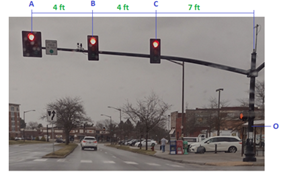
\includegraphics{images/stoplights.png}

}

\caption{Figure 1: Three traffic light installation with loads}

\end{figure}%

\section*{Worked Out Solution}\label{worked-out-solution}
\addcontentsline{toc}{section}{Worked Out Solution}

\markright{Worked Out Solution}

This demonstrates a worked out solution to the problem. The best way to
begin is by drawing a free body diagram.

\begin{figure}[H]

{\centering 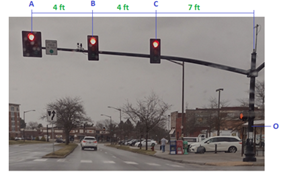
\includegraphics{images/stoplights.png}

}

\caption{Figure 3: Three traffic light installation with loads}

\end{figure}%

Use equilibrium equations to find the internal loads:

\[
\Sigma F_y=0: N-65-50-50=0
\] \[N=165~lbs
\]

\[
\Sigma M_O=0: -M+(50\times7)+(50\times11)+(65\times15)=0
\] \[
M=1875~lb\cdot ft=22500~lb\cdot in
\]

Now, determine the cross-sectional properties:

\[
A=\pi(r_0^2-r_i^2)=\pi(2.5^2-2.3^2)=3.02~in^2
\] \[
I=
\frac{\pi}{4}
(r_0^4-r_i^4)=\frac{\pi}{4}(2.5^4-2.3^4)=8.70~in^4
\]

Calculate stress due to normal force:

\[
\sigma_n=\frac{F}{A}=\frac{-165~lbs}{3.02~in^2}=-54.7~psi
\]

Calculate maximum stress due to bending moment (will have same magnitude
in both tension and compression):

\[
\sigma_m=\pm\frac{M_c}{I}=\pm\frac{22500\times2.5}{8.70}=\pm6460~psi
\]

Determine combined tensile stress: \(\sigma_T=-54.7+6460=6410~psi\)

Determine combined compressive stress: \(\sigma_T=-54.7-6460=-6520~psi\)

\chapter*{Dynamic Problem Statement}\label{dynamic-problem-statement}
\addcontentsline{toc}{chapter}{Dynamic Problem Statement}

\markboth{Dynamic Problem Statement}{Dynamic Problem Statement}

This is a dynamic rendering of the problem with dynamic variables based
on the username entered. Please note at this time that the figure
displays incorrect values. This will be corrected when drawn by the
graphic artist.

\section*{Problem Image}\label{problem-image}
\addcontentsline{toc}{section}{Problem Image}

\markright{Problem Image}

\begin{figure}[H]

{\centering 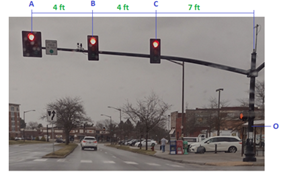
\includegraphics{images/stoplights.png}

}

\caption{Figure 1: Three traffic light installation with loads}

\end{figure}%

\begin{Shaded}
\begin{Highlighting}[]
\NormalTok{\#| standalone: true}
\NormalTok{\#| viewerHeight: 600}
\NormalTok{\#| components: [viewer]}

\NormalTok{from shiny import App, render, ui, reactive}
\NormalTok{import random}
\NormalTok{import asyncio}
\NormalTok{import io}
\NormalTok{import math}
\NormalTok{from datetime import datetime}
\NormalTok{from pathlib import Path}

\NormalTok{problem\_ID="1"}
\NormalTok{light\_a=reactive.Value("\_\_")}
\NormalTok{lights\_bc=reactive.Value("\_\_")}
\NormalTok{attempts=["Timestamp,Attempt,Answer,Feedback\textbackslash{}n"]}

\NormalTok{app\_ui = ui.page\_fluid(}
\NormalTok{    ui.markdown("**Please enter your ID number from your instructor and click to generate your problem**"),}
\NormalTok{    ui.input\_text("ID","", placeholder="Enter ID Number Here"),}
\NormalTok{    ui.input\_action\_button("generate\_problem", "Generate Problem", class\_="btn{-}primary"),}
\NormalTok{    ui.markdown("**Problem Statement**"),}
\NormalTok{    ui.output\_ui("ui\_problem\_statement"),}
\NormalTok{    ui.input\_text("answer","Your Answer in units of psi", placeholder="Please enter your answer"),}
\NormalTok{    ui.input\_action\_button("submit", "Submit Answer", class\_="btn{-}primary"),}
\NormalTok{    ui.download\_button("download", "Download File to Submit", class\_="btn{-}success"),}
\NormalTok{)}


\NormalTok{def server(input, output, session):}
\NormalTok{    @output}
\NormalTok{    @render.ui}
\NormalTok{    def ui\_problem\_statement():}
\NormalTok{        return[ui.markdown(f"A city planner is installing a new traffic light. Light A weighs \{light\_a()\} lb, while lights B and C weigh \{lights\_bc()\} lb each. The post at O has a hollow circular cross{-}section with an outer diameter of 5 inches and a wall thickness of 0.2 inches. Please calculate the magnitude of the maximum combined stress in the post. You may ignore the weight of the post.")]}
    
\NormalTok{    @reactive.Effect}
\NormalTok{    @reactive.event(input.generate\_problem)}
\NormalTok{    def randomize\_vars():}
\NormalTok{        random.seed(input.ID())}
\NormalTok{        light\_a.set(round(65+65*(.5{-}random.random())*.2))}
\NormalTok{        lights\_bc.set(round(50+50*(.5{-}random.random())*.2))}

\NormalTok{    @reactive.Effect}
\NormalTok{    @reactive.event(input.submit)}
\NormalTok{    def \_():}
\NormalTok{        instr= (light\_a()+2*lights\_bc()/math.pi*(2.5**2 {-} 2.3**2))+ (({-}1*lights\_bc()*7{-} lights\_bc()*11 {-} light\_a()*15)*12*2.5)/ ((math.pi/4)*(2.5**4 {-} 2.3**4))}
\NormalTok{        \#check=math.isclose(float(input.answer()),instr,rel\_tol=0.001)}
\NormalTok{        if math.isclose(float(input.answer()),instr,rel\_tol=0.001):}
\NormalTok{           check="*Correct*"}
\NormalTok{        else:}
\NormalTok{           check="*Not Correct.*"}
        
\NormalTok{        if check=="*Not Correct.*" and math.isclose(abs(float(input.answer())),abs(instr),rel\_tol=0.001):}
\NormalTok{           extra\_check="An extra check says you may have a sign error."}
\NormalTok{        else:}
\NormalTok{           extra\_check=""}
\NormalTok{        \#extra\_check = "An extra check says you may have a sign error." if math.isclose(abs(input.answer()),abs(instr,rel\_tol=0.001)) else ""}
\NormalTok{        feedback=ui.markdown(f"Your answer of \{input.answer()\} is \{check\} \{extra\_check\} For reference in debugging this, the calculated instructor answer is \{instr\}")}
\NormalTok{        attempts.append(f"\{datetime.now()\}, \{input.submit()\},\{input.answer()\},\{check\}\textbackslash{}n")}
\NormalTok{        m=ui.modal(}
\NormalTok{          feedback,}
\NormalTok{          title="Feedback",}
\NormalTok{          easy\_close=True}
\NormalTok{        )}
\NormalTok{        ui.modal\_show(m)}
        
\NormalTok{    @session.download(}
\NormalTok{        filename=lambda: f"Problem\_Log{-}\{problem\_ID\}{-}\{input.ID()\}.csv"}
\NormalTok{    )}
\NormalTok{    async def download():}
\NormalTok{        \# This version uses a function to generate the filename. It also yields data}
\NormalTok{        \# multiple times.}
\NormalTok{        await asyncio.sleep(0.25)}
\NormalTok{        yield f"\{problem\_ID\}\_\{input.submit()\}\_\{input.ID()\}\textbackslash{}n"}
\NormalTok{        yield \textquotesingle{}\textquotesingle{}.join(attempts)}
           

\NormalTok{app = App(app\_ui, server)}
\end{Highlighting}
\end{Shaded}

\chapter*{Interactive Problem
Interface}\label{interactive-problem-interface}
\addcontentsline{toc}{chapter}{Interactive Problem Interface}

\markboth{Interactive Problem Interface}{Interactive Problem Interface}

To scaffold your learning in this example, we have provided a free body
diagram for you and a repeat of the problem statement.

A city planner is installing a new traffic light. Light A weighs 65 lb,
while lights B and C weigh 50 lb each. The post at O has a hollow
circular cross-section with an outer diameter of 5 inches and a wall
thickness of 0.2 inches. Please calculate the magnitude of the maximum
combined stress in the post. You may ignore the weight of the post.

\begin{figure}[H]

{\centering 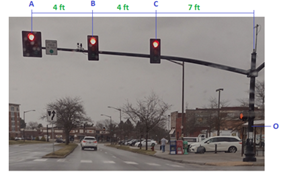
\includegraphics{images/stoplights.png}

}

\caption{Figure 1: Three traffic light installation with loads}

\end{figure}%

Please work through the problem step by step showing your math in the
interactive interface here.

\begin{Shaded}
\begin{Highlighting}[]
\NormalTok{\#| standalone: true}
\NormalTok{\#| viewerHeight: 600}
\NormalTok{\#| components: [viewer]}



\NormalTok{import io}
\NormalTok{import numpy as np}
\NormalTok{import asyncio}
\NormalTok{from datetime import datetime}
\NormalTok{from pathlib import Path}
\NormalTok{import matplotlib.pyplot as plt}
\NormalTok{from shiny import App, render, ui, reactive, req}
\NormalTok{from sympy import solve, Eq, Symbol}
\NormalTok{from sympy.parsing.sympy\_parser import parse\_expr}
\NormalTok{from shiny.ui import h4}

\NormalTok{\# load equations lists}


\NormalTok{class eqn:}
\NormalTok{    def \_\_init\_\_(self, name, inline\_math, newline\_math, working\_sym, working\_eqn\_latex,working\_eqn\_solver):}
\NormalTok{        self.name = name}
\NormalTok{        self.inline\_math = inline\_math}
\NormalTok{        self.newline\_math = newline\_math}
\NormalTok{        self.working\_sym = working\_sym}
\NormalTok{        self.working\_eqn\_latex = working\_eqn\_latex}
\NormalTok{        self.working\_eqn\_solver = working\_eqn\_solver}

\NormalTok{StaticsSumFx = eqn(}
\NormalTok{    "Equilibrium Forces in X", }
\NormalTok{    "\textbackslash{}(\textbackslash{}Sigma F\_x=0\textbackslash{})", }
\NormalTok{    "$$\textbackslash{}Sigma F\_x=0$$", }
\NormalTok{    "SigmaFx",}
\NormalTok{    "$$F\_x1+F\_x2+F\_x3+F\_x4+F\_x5=0$$",}
\NormalTok{    "F\_x1+F\_x2+F\_x3+F\_x4+F\_x5=0"}
\NormalTok{)}

\NormalTok{StaticsSumFy = eqn(}
\NormalTok{    "Equilibrium Forces in Y", }
\NormalTok{    "\textbackslash{}(\textbackslash{}Sigma F\_y=0\textbackslash{})", }
\NormalTok{    "$$\textbackslash{}Sigma F\_y=0$$", }
\NormalTok{    "SigmaFy",}
\NormalTok{    "$$F\_y1+F\_y2+F\_y3+F\_y4+F\_y5=0$$",}
\NormalTok{    "F\_y1+F\_y2+F\_y3+F\_y4+F\_y5=0"}
\NormalTok{)}

\NormalTok{StaticsSumM = eqn(}
\NormalTok{    "Equilibrium Moments about O", }
\NormalTok{    "\textbackslash{}(\textbackslash{}Sigma M\_O=0\textbackslash{})", }
\NormalTok{    "$$\textbackslash{}Sigma M\_O=0$$", }
\NormalTok{    "SigmaM",}
\NormalTok{    "$$M\_1+M\_2+M\_3+M\_4+M\_5=0$$",}
\NormalTok{    "M\_1+M\_2+M\_3+M\_4+M\_5=0"}
\NormalTok{)}

\NormalTok{StressEqn = eqn(}
\NormalTok{    "Stress Equation", }
\NormalTok{    "\textbackslash{}(\textbackslash{}sigma=\textbackslash{}\textbackslash{}frac\{F\}\{A\}\textbackslash{})", }
\NormalTok{    "$$\textbackslash{}sigma=\textbackslash{}\textbackslash{}frac\{F\}\{A\}$$", }
\NormalTok{    "sigma,F,A",}
\NormalTok{    "$$\textbackslash{}sigma=\textbackslash{}\textbackslash{}frac\{(F)\}\{(A)\}$$",}
\NormalTok{    "Eq(sigma,(F)/(A))"}
\NormalTok{)}

\NormalTok{AxialDeform = eqn(}
\NormalTok{    "Axial Deformation by Force",}
\NormalTok{    "\textbackslash{}(\textbackslash{}delta\_l=\textbackslash{}\textbackslash{}frac\{P L\}\{AE\}\textbackslash{})",}
\NormalTok{    "$$\textbackslash{}delta\_l=\textbackslash{}\textbackslash{}frac\{P\textbackslash{}cdot L\}\{A \textbackslash{}cdot E\}$$",}
\NormalTok{    "delta\_l,P,L,A,E",}
\NormalTok{    "$$\textbackslash{}delta\_l=\textbackslash{}\textbackslash{}frac\{(P)(L)\}\{(A)(E)\}$$",}
\NormalTok{    "Eq(delta\_l,(P)*(L)/(A)/(E))"}
\NormalTok{)}

\NormalTok{ThermalDeform = eqn(}
\NormalTok{    "Axial Deformation by Thermal",}
\NormalTok{    "\textbackslash{}(\textbackslash{}delta\_t= \textbackslash{}\textbackslash{}alpha \textbackslash{}Delta T L\textbackslash{})",}
\NormalTok{    "$$\textbackslash{}delta\_t= \textbackslash{}\textbackslash{}alpha \textbackslash{}cdot \textbackslash{}Delta T \textbackslash{}cdot L$$",}
\NormalTok{    "delta\_t,alpha,DeltaT,L",}
\NormalTok{    "$$\textbackslash{}delta\_t= \textbackslash{}\textbackslash{}alpha \textbackslash{}Delta T L$$",}
\NormalTok{    "delta\_t= alpha*(Delta\_T)*L"}
\NormalTok{)}

\NormalTok{AreaTube = eqn(}
\NormalTok{    "Area of a Tube", }
\NormalTok{    "\textbackslash{}(A\_\{tube\}=\textbackslash{}pi(r\_o\^{}2{-}r\_i\^{}2)\textbackslash{})", }
\NormalTok{    "$$A\_\{tube\}=\textbackslash{}pi(r\_o\^{}2{-}r\_i\^{}2)$$", }
\NormalTok{    "A\_tube,r\_o,r\_i",}
\NormalTok{    "$$A\_\{tube\}=\textbackslash{}pi(r\_o\^{}2{-}r\_i\^{}2)$$",}
\NormalTok{    "Eq(A\_tube,pi*((r\_o)**2{-}(r\_i)**2))"}
\NormalTok{)}

\NormalTok{ITube = eqn(}
\NormalTok{    "Moment of Inertia of a Tube",}
\NormalTok{    "\textbackslash{}(I\_\{tube\}=\textbackslash{}\textbackslash{}frac\{\textbackslash{}pi\}\{4\}(r\_o\^{}4{-}r\_i\^{}4)\textbackslash{})",}
\NormalTok{    "$$I\_\{tube\}=\textbackslash{}\textbackslash{}frac\{\textbackslash{}pi\}\{4\}(r\_o\^{}4{-}r\_i\^{}4)$$",}
\NormalTok{    "I\_tube,r\_o,r\_i",}
\NormalTok{    "$$I\_\{tube\}=\textbackslash{}\textbackslash{}frac\{\textbackslash{}pi\}\{4\}(r\_o\^{}4{-}r\_i\^{}4)$$", }
\NormalTok{    "Eq(I\_tube,pi/4*((r\_o)**4{-}(r\_i)**4))" }
\NormalTok{)}

\NormalTok{BendingStress = eqn(}
\NormalTok{    "Bending Stress from a Moment",}
\NormalTok{    "\textbackslash{}(\textbackslash{}sigma\_b=\textbackslash{}\textbackslash{}frac\{M*y\}\{I\}\textbackslash{})",}
\NormalTok{    "$$\textbackslash{}sigma\_b=\textbackslash{}\textbackslash{}frac\{M*y\}\{I\}$$",}
\NormalTok{    "sigma\_b,M,y,I,",}
\NormalTok{    "$$\textbackslash{}sigma\_b=\textbackslash{}\textbackslash{}frac\{M*y\}\{I\}$$", }
\NormalTok{    "Eq(sigma\_b,M*y/I))" }
\NormalTok{)}

\NormalTok{Compatability1 = eqn(}
\NormalTok{    "Compatability Equation 1",}
\NormalTok{    "\textbackslash{}(a\_1+\textbackslash{}ldots=b\_1+b\_2+\textbackslash{}ldots\textbackslash{})", }
\NormalTok{    "$$a\_1+\textbackslash{}ldots=b\_1+b\_2+\textbackslash{}ldots$$", }
\NormalTok{    "",}
\NormalTok{    "$$a\_1+a\_n=b\_1+b\_n$$",}
\NormalTok{    "Eq(a\_1+a\_n=b\_1+b\_n)" }
\NormalTok{)}

\NormalTok{Compatability2 = eqn(}
\NormalTok{    "Compatability Equation 2",}
\NormalTok{    "\textbackslash{}(c\_1+\textbackslash{}ldots=d\_1+d\_2+\textbackslash{}ldots\textbackslash{})", }
\NormalTok{    "$$c\_1+\textbackslash{}ldots=d\_1+d\_2+\textbackslash{}ldots$$", }
\NormalTok{    "",}
\NormalTok{    "$$c\_1+c\_n=d\_1+d\_n$$",}
\NormalTok{    "Eq(c\_1+c\_n=d\_1+d\_n)" }
\NormalTok{)}


\NormalTok{statics\_eqnbank\_inline = \{}
\NormalTok{    StaticsSumFx.name: StaticsSumFx.inline\_math,}
\NormalTok{    StaticsSumFy.name: StaticsSumFy.inline\_math,}
\NormalTok{    StaticsSumM.name: StaticsSumM.inline\_math,}
\NormalTok{\}}
\NormalTok{deforms\_eqnbank\_inline = \{}
\NormalTok{    StressEqn.name: StressEqn.inline\_math,}
\NormalTok{    AxialDeform.name: AxialDeform.inline\_math,}
\NormalTok{    ThermalDeform.name: ThermalDeform.inline\_math,}
\NormalTok{\}}

\NormalTok{geom\_eqnbank\_inline = \{}
\NormalTok{    AreaTube.name: AreaTube.inline\_math,}
\NormalTok{    ITube.name: ITube.inline\_math,}
\NormalTok{\}}

\NormalTok{eqnbank\_inline = \{}
\NormalTok{    StaticsSumFx.name: StaticsSumFx.inline\_math,}
\NormalTok{    StaticsSumFy.name: StaticsSumFy.inline\_math,}
\NormalTok{    StaticsSumM.name: StaticsSumM.inline\_math,}
\NormalTok{    StressEqn.name: StressEqn.inline\_math,}
\NormalTok{    BendingStress.name: BendingStress.inline\_math,}
\NormalTok{    AxialDeform.name: AxialDeform.inline\_math,}
\NormalTok{    ThermalDeform.name: ThermalDeform.inline\_math,}
\NormalTok{    AreaTube.name: AreaTube.inline\_math,}
\NormalTok{    ITube.name: ITube.inline\_math,}
\NormalTok{    Compatability1.name: Compatability1.inline\_math,}
\NormalTok{    Compatability2.name: Compatability2.inline\_math,}
\NormalTok{\}}

\NormalTok{eqnbank\_newline = \{}
\NormalTok{    StaticsSumFx.name: StaticsSumFx.newline\_math,}
\NormalTok{    StaticsSumFy.name: StaticsSumFy.newline\_math,}
\NormalTok{    StaticsSumM.name: StaticsSumM.newline\_math,}
\NormalTok{    StressEqn.name: StressEqn.newline\_math,}
\NormalTok{    BendingStress.name: BendingStress.newline\_math,}
\NormalTok{    AxialDeform.name: AxialDeform.newline\_math,}
\NormalTok{    ThermalDeform.name: ThermalDeform.newline\_math,}
\NormalTok{    AreaTube.name: AreaTube.newline\_math,}
\NormalTok{    ITube.name: ITube.newline\_math,}
\NormalTok{    Compatability1.name: Compatability1.newline\_math,}
\NormalTok{    Compatability2.name: Compatability2.newline\_math,}
\NormalTok{\}}



\NormalTok{working\_equations\_solver=reactive.Value([])}
\NormalTok{working\_equations\_latex\_render=reactive.Value([])}
\NormalTok{working\_symbols=reactive.Value([])}

\NormalTok{feedback\_equations=reactive.Value([])}
\NormalTok{feedback\_solns=reactive.Value([])}
\NormalTok{feedback\_syms=reactive.Value([])}

\NormalTok{working\_SumFx\_render=reactive.Value("")}
\NormalTok{working\_SumFy\_render=reactive.Value("")}
\NormalTok{working\_SumM\_render=reactive.Value("")}
\NormalTok{working\_StressEqn\_render=reactive.Value("")}
\NormalTok{working\_BendingStress\_render=reactive.Value("")}
\NormalTok{working\_AxialDeform\_render=reactive.Value("")}
\NormalTok{working\_ThermalDeform\_render=reactive.Value("")}
\NormalTok{working\_AreaTube\_render=reactive.Value("")}
\NormalTok{working\_Itube\_render=reactive.Value("")}
\NormalTok{working\_Compatability1\_render=reactive.Value("")}
\NormalTok{working\_Compatability2\_render=reactive.Value("")}

\NormalTok{working\_SumFx\_string=reactive.Value("")}
\NormalTok{working\_SumFy\_string=reactive.Value("")}
\NormalTok{working\_SumM\_string=reactive.Value("")}
\NormalTok{working\_StressEqn\_string=reactive.Value("")}
\NormalTok{working\_BendingStress\_string=reactive.Value("")}
\NormalTok{working\_AxialDeform\_string=reactive.Value("")}
\NormalTok{working\_ThermalDeform\_string=reactive.Value("")}
\NormalTok{working\_AreaTube\_string=reactive.Value("")}
\NormalTok{working\_Itube\_string=reactive.Value("")}
\NormalTok{working\_Compatability1\_string=reactive.Value("")}
\NormalTok{working\_Compatability2\_string=reactive.Value("")}

\NormalTok{NumForcesY=reactive.Value(2)}
\NormalTok{F1y=reactive.Value("")}
\NormalTok{F2y=reactive.Value("")}
\NormalTok{F3y=reactive.Value("")}
\NormalTok{F4y=reactive.Value("")}
\NormalTok{F5y=reactive.Value("")}
\NormalTok{Equil\_latex=reactive.Value("")}

\NormalTok{NumForcesX=reactive.Value(2)}
\NormalTok{F1x=reactive.Value("")}
\NormalTok{F2x=reactive.Value("")}
\NormalTok{F3x=reactive.Value("")}
\NormalTok{F4x=reactive.Value("")}
\NormalTok{F5x=reactive.Value("")}

\NormalTok{NumMoments=reactive.Value(2)}
\NormalTok{M1=reactive.Value("")}
\NormalTok{M2=reactive.Value("")}
\NormalTok{M3=reactive.Value("")}
\NormalTok{M4=reactive.Value("")}
\NormalTok{M5=reactive.Value("")}

\NormalTok{axial\_stress\_sigma=reactive.Value("")}
\NormalTok{axial\_stress\_force=reactive.Value("")}
\NormalTok{axial\_stress\_area=reactive.Value("")}

\NormalTok{bending\_stress\_sigma=reactive.Value("")}
\NormalTok{bending\_stress\_M=reactive.Value("")}
\NormalTok{bending\_stress\_y=reactive.Value("")}
\NormalTok{bending\_stress\_I=reactive.Value("")}

\NormalTok{axial\_delta\_l=reactive.Value("")}
\NormalTok{axial\_P=reactive.Value("")}
\NormalTok{axial\_L=reactive.Value("")}
\NormalTok{axial\_A=reactive.Value("")}
\NormalTok{axial\_E=reactive.Value("")}

\NormalTok{thermal\_delta\_t=reactive.Value("")}
\NormalTok{thermal\_alpha=reactive.Value("")}
\NormalTok{thermal\_Delta\_T=reactive.Value("")}
\NormalTok{thermal\_L=reactive.Value("")}

\NormalTok{area\_tube\_A\_tube=reactive.Value("")}
\NormalTok{area\_tube\_Ar\_o=reactive.Value("")}
\NormalTok{area\_tube\_Ar\_i=reactive.Value("")}

\NormalTok{I\_tube\_I\_tube=reactive.Value("")}
\NormalTok{I\_tube\_Ir\_o=reactive.Value("")}
\NormalTok{i\_tube\_Ir\_i=reactive.Value("")}

\NormalTok{Compatability1\_NumLHS=reactive.Value(1)}
\NormalTok{Compatability1\_NumRHS=reactive.Value(2)}
\NormalTok{Compatability1\_a\_1=reactive.Value("")}
\NormalTok{Compatability1\_a\_2=reactive.Value("")}
\NormalTok{Compatability1\_a\_3=reactive.Value("")}
\NormalTok{Compatability1\_a\_4=reactive.Value("")}
\NormalTok{Compatability1\_a\_5=reactive.Value("")}
\NormalTok{Compatability1\_b\_1=reactive.Value("")}
\NormalTok{Compatability1\_b\_2=reactive.Value("")}
\NormalTok{Compatability1\_b\_3=reactive.Value("")}
\NormalTok{Compatability1\_b\_4=reactive.Value("")}
\NormalTok{Compatability1\_b\_5=reactive.Value("")}

\NormalTok{Compatability2\_NumLHS=reactive.Value(1)}
\NormalTok{Compatability2\_NumRHS=reactive.Value(2)}
\NormalTok{Compatability2\_c\_1=reactive.Value("")}
\NormalTok{Compatability2\_c\_2=reactive.Value("")}
\NormalTok{Compatability2\_c\_3=reactive.Value("")}
\NormalTok{Compatability2\_c\_4=reactive.Value("")}
\NormalTok{Compatability2\_c\_5=reactive.Value("")}
\NormalTok{Compatability2\_d\_1=reactive.Value("")}
\NormalTok{Compatability2\_d\_2=reactive.Value("")}
\NormalTok{Compatability2\_d\_3=reactive.Value("")}
\NormalTok{Compatability2\_d\_4=reactive.Value("")}
\NormalTok{Compatability2\_d\_5=reactive.Value("")}

\NormalTok{active\_eqn\_tab=reactive.Value("Instructions")}

\NormalTok{prob\_statement="To scaffold your learning in this example, we have provided a free body diagram for you and a repeat of the problem statement. A city planner is installing a new traffic light. Light A weighs 65 lb, while lights B and C weigh 50 lb each. The post at O has a hollow circular cross{-}section with an outer diameter of 5 inches and a wall thickness of 0.2 inches. Please calculate the magnitude of the maximum combined stress in the post. You may ignore the weight of the post."}

\NormalTok{app\_ui = ui.page\_fluid(}
\NormalTok{    ui.head\_content(}
\NormalTok{        ui.tags.script(}
\NormalTok{            src="https://mathjax.rstudio.com/latest/MathJax.js?config=TeX{-}AMS{-}MML\_HTMLorMML"}
\NormalTok{        ),}
\NormalTok{        ui.tags.script(}
\NormalTok{            "if (window.MathJax) MathJax.Hub.Queue([\textquotesingle{}Typeset\textquotesingle{}, MathJax.Hub]);"}
\NormalTok{        ),}
\NormalTok{    ),}
\NormalTok{    ui.panel\_title("Interactive Problem Solving Environment"),}
\NormalTok{        ui.row(}
\NormalTok{            ui.column(6,}
\NormalTok{                ui.markdown("**Problem Statement**"),}
\NormalTok{                ui.markdown(prob\_statement),}
\NormalTok{                ),}
\NormalTok{            ui.column(6,ui.output\_ui("dyn\_ui\_nav")),}
\NormalTok{            ),}
\NormalTok{        \#ui.row(}
\NormalTok{        \#    ui.output\_ui("dyn\_ui\_nav"),}
\NormalTok{        \#    ),}
\NormalTok{        ui.row(}
\NormalTok{            ui.markdown("**Your Equation Workspace**"),}
\NormalTok{            \#ui.column(6,ui.output\_ui("dyn\_ui\_nav")),}
\NormalTok{            ui.column(4,}
\NormalTok{                ui.navset\_tab\_card(}
\NormalTok{                    ui.nav("Equation Bank",}
\NormalTok{                        ui.input\_checkbox\_group("selected\_eqns","Choose your equations:",eqnbank\_inline,}
\NormalTok{                        ),}
\NormalTok{                    ),}
\NormalTok{                ),}
\NormalTok{            ),}
\NormalTok{            ui.column(2,ui.output\_ui("dyn\_eqns"),style=\textquotesingle{}border{-}right:1px solid;\textquotesingle{}),}
\NormalTok{            ui.column(4,ui.output\_ui("dyn\_working\_eqns"),ui.output\_text("txt")),}
\NormalTok{        ),}
\NormalTok{        ui.row(}
\NormalTok{          ui.output\_ui("ui\_equation\_bookkeeping")}
\NormalTok{        ),}
\NormalTok{        \#ui.row(ui.input\_action\_button(}
\NormalTok{        \#            "solveEquations", "Solve Equations", class\_="btn{-}success", width="240px", style=\textquotesingle{}margin{-}bottom:10px\textquotesingle{})}
\NormalTok{        \#      ),}
\NormalTok{        ui.output\_ui("ui\_solutions"),}
\NormalTok{)}


\NormalTok{def server(input, output, session):}
   
\NormalTok{    @output}
\NormalTok{    @render.ui}
\NormalTok{    def dyn\_eqns():}
\NormalTok{        eqns\_keys = input.selected\_eqns()}
\NormalTok{        req(eqns\_keys)}
\NormalTok{        lookup\_eqns = [eqnbank\_newline[key] for key in eqns\_keys]}
\NormalTok{        mystring\_eqns = "".join(lookup\_eqns)}
\NormalTok{        feedback\_equations.set(lookup\_eqns)}

\NormalTok{        return [}
\NormalTok{            ui.markdown(mystring\_eqns),}
\NormalTok{            ui.tags.script(}
\NormalTok{                "if (window.MathJax) MathJax.Hub.Queue([\textquotesingle{}Typeset\textquotesingle{}, MathJax.Hub]);"}
\NormalTok{            ),}
\NormalTok{        ]}

\NormalTok{    @output}
\NormalTok{    @render.ui}
\NormalTok{    def dyn\_working\_eqns():}
\NormalTok{        eqns\_keys = input.selected\_eqns()}
\NormalTok{        req(eqns\_keys)}
\NormalTok{        lookup\_eqns = [eqnbank\_newline[key] for key in eqns\_keys]}
        

\NormalTok{        \# Dynamic Filling of Force equations }
\NormalTok{        if StaticsSumFy.newline\_math in lookup\_eqns:}
\NormalTok{            StaticsSumFy\_list = ["F\_y1","F\_y2","F\_y3","F\_y4","F\_y5"]}
\NormalTok{            StaticsSumFy\_list = StaticsSumFy\_list[:input.NumForcesY()]}
\NormalTok{            StaticsSumFy.working\_sym = ",".join(StaticsSumFy\_list)}
\NormalTok{            StaticsSumFy.working\_eqn\_latex = "$$" + "+".join(StaticsSumFy\_list) + "=0$$"}
\NormalTok{            StaticsSumFy.working\_eqn\_solver = "+".join(StaticsSumFy\_list)}
            
\NormalTok{            if str(input.F1y()) != "" : }
\NormalTok{                StaticsSumFy.working\_eqn\_latex = StaticsSumFy.working\_eqn\_latex.replace("F\_y1",str(input.F1y()))}
\NormalTok{                StaticsSumFy.working\_sym = StaticsSumFy.working\_sym.replace("F\_y1",str(input.F1y()))}
\NormalTok{                StaticsSumFy.working\_eqn\_solver = StaticsSumFy.working\_eqn\_solver.replace("F\_y1",str(input.F1y()))}
\NormalTok{            else:}
\NormalTok{                StaticsSumFy.working\_eqn\_latex = StaticsSumFy.working\_eqn\_latex.replace("F\_y1","\textbackslash{}\textbackslash{}boxed\{F\_\{y\_1\}\}")}
        
\NormalTok{            if str(input.F2y()) != "" : }
\NormalTok{                StaticsSumFy.working\_eqn\_latex = StaticsSumFy.working\_eqn\_latex.replace("F\_y2",str(input.F2y()))}
\NormalTok{                StaticsSumFy.working\_sym = StaticsSumFy.working\_sym.replace("F\_y2",str(input.F2y()))}
\NormalTok{                StaticsSumFy.working\_eqn\_solver = StaticsSumFy.working\_eqn\_solver.replace("F\_y2",str(input.F2y()))}
\NormalTok{            else:}
\NormalTok{                StaticsSumFy.working\_eqn\_latex = StaticsSumFy.working\_eqn\_latex.replace("F\_y2","\textbackslash{}\textbackslash{}boxed\{F\_\{y\_2\}\}")}
        
\NormalTok{            if str(input.F3y()) != "" : }
\NormalTok{                StaticsSumFy.working\_eqn\_latex = StaticsSumFy.working\_eqn\_latex.replace("F\_y3",str(input.F3y()))}
\NormalTok{                StaticsSumFy.working\_sym = StaticsSumFy.working\_sym.replace("F\_y3",str(input.F3y()))}
\NormalTok{                StaticsSumFy.working\_eqn\_solver = StaticsSumFy.working\_eqn\_solver.replace("F\_y3",str(input.F3y()))}
\NormalTok{            else:}
\NormalTok{                StaticsSumFy.working\_eqn\_latex = StaticsSumFy.working\_eqn\_latex.replace("F\_y3","\textbackslash{}\textbackslash{}boxed\{F\_\{y\_3\}\}")}
        
\NormalTok{            if str(input.F4y()) != "" : }
\NormalTok{                StaticsSumFy.working\_eqn\_latex = StaticsSumFy.working\_eqn\_latex.replace("F\_y4",str(input.F4y()))}
\NormalTok{                StaticsSumFy.working\_sym = StaticsSumFy.working\_sym.replace("F\_y4",str(input.F4y()))}
\NormalTok{                StaticsSumFy.working\_eqn\_solver = StaticsSumFy.working\_eqn\_solver.replace("F\_y4",str(input.F4y()))}
\NormalTok{            else:}
\NormalTok{                StaticsSumFy.working\_eqn\_latex = StaticsSumFy.working\_eqn\_latex.replace("F\_y4","\textbackslash{}\textbackslash{}boxed\{F\_\{y\_4\}\}")}
        
\NormalTok{            if str(input.F5y()) != "" : }
\NormalTok{                StaticsSumFy.working\_eqn\_latex = StaticsSumFy.working\_eqn\_latex.replace("F\_y5",str(input.F5y()))}
\NormalTok{                StaticsSumFy.working\_sym = StaticsSumFy.working\_sym.replace("F\_y5",str(input.F5y()))}
\NormalTok{                StaticsSumFy.working\_eqn\_solver = StaticsSumFy.working\_eqn\_solver.replace("F\_y5",str(input.F5y()))}
\NormalTok{            else:}
\NormalTok{                StaticsSumFy.working\_eqn\_latex = StaticsSumFy.working\_eqn\_latex.replace("F\_y5","\textbackslash{}\textbackslash{}boxed\{F\_\{y\_5\}\}")}
      
\NormalTok{  \# Dynamic Filling of Force equations }
\NormalTok{        if StaticsSumFx.newline\_math in lookup\_eqns:}
\NormalTok{            StaticsSumFx\_list = ["F\_x1","F\_x2","F\_x3","F\_x4","F\_x5"]}
\NormalTok{            StaticsSumFx\_list = StaticsSumFx\_list[:input.NumForcesX()]}
\NormalTok{            StaticsSumFx.working\_sym = ",".join(StaticsSumFx\_list)}
\NormalTok{            StaticsSumFx.working\_eqn\_latex = "$$" + "+".join(StaticsSumFx\_list) + "=0$$"}
\NormalTok{            StaticsSumFx.working\_eqn\_solver = "+".join(StaticsSumFx\_list)}
            
\NormalTok{            if str(input.F1x()) != "" : }
\NormalTok{                StaticsSumFx.working\_eqn\_latex = StaticsSumFx.working\_eqn\_latex.replace("F\_x1",str(input.F1x()))}
\NormalTok{                StaticsSumFx.working\_sym = StaticsSumFx.working\_sym.replace("F\_x1",str(input.F1x()))}
\NormalTok{                StaticsSumFx.working\_eqn\_solver = StaticsSumFx.working\_eqn\_solver.replace("F\_x1",str(input.F1x()))}
\NormalTok{            else:}
\NormalTok{                StaticsSumFx.working\_eqn\_latex = StaticsSumFx.working\_eqn\_latex.replace("F\_x1","\textbackslash{}\textbackslash{}boxed\{F\_\{x\_1\}\}")}
        
\NormalTok{            if str(input.F2x()) != "" : }
\NormalTok{                StaticsSumFx.working\_eqn\_latex = StaticsSumFx.working\_eqn\_latex.replace("F\_x2",str(input.F2x()))}
\NormalTok{                StaticsSumFx.working\_sym = StaticsSumFx.working\_sym.replace("F\_x2",str(input.F2x()))}
\NormalTok{                StaticsSumFx.working\_eqn\_solver = StaticsSumFx.working\_eqn\_solver.replace("F\_x2",str(input.F2x()))}
\NormalTok{            else:}
\NormalTok{                StaticsSumFx.working\_eqn\_latex = StaticsSumFx.working\_eqn\_latex.replace("F\_x2","\textbackslash{}\textbackslash{}boxed\{F\_\{x\_2\}\}")}
        
\NormalTok{            if str(input.F3x()) != "" : }
\NormalTok{                StaticsSumFx.working\_eqn\_latex = StaticsSumFx.working\_eqn\_latex.replace("F\_x3",str(input.F3x()))}
\NormalTok{                StaticsSumFx.working\_sym = StaticsSumFx.working\_sym.replace("F\_x3",str(input.F3x()))}
\NormalTok{                StaticsSumFx.working\_eqn\_solver = StaticsSumFx.working\_eqn\_solver.replace("F\_x3",str(input.F3x()))}
\NormalTok{            else:}
\NormalTok{                StaticsSumFx.working\_eqn\_latex = StaticsSumFx.working\_eqn\_latex.replace("F\_x3","\textbackslash{}\textbackslash{}boxed\{F\_\{x\_3\}\}")}
        
\NormalTok{            if str(input.F4x()) != "" : }
\NormalTok{                StaticsSumFx.working\_eqn\_latex = StaticsSumFx.working\_eqn\_latex.replace("F\_x4",str(input.F4x()))}
\NormalTok{                StaticsSumFx.working\_sym = StaticsSumFx.working\_sym.replace("F\_x4",str(input.F4x()))}
\NormalTok{                StaticsSumFx.working\_eqn\_solver = StaticsSumFx.working\_eqn\_solver.replace("F\_x4",str(input.F4x()))}
\NormalTok{            else:}
\NormalTok{                StaticsSumFx.working\_eqn\_latex = StaticsSumFx.working\_eqn\_latex.replace("F\_x4","\textbackslash{}\textbackslash{}boxed\{F\_\{x\_4\}\}")}
        
\NormalTok{            if str(input.F5x()) != "" : }
\NormalTok{                StaticsSumFx.working\_eqn\_latex = StaticsSumFx.working\_eqn\_latex.replace("F\_x5",str(input.F5x()))}
\NormalTok{                StaticsSumFx.working\_sym = StaticsSumFx.working\_sym.replace("F\_x5",str(input.F5x()))}
\NormalTok{                StaticsSumFx.working\_eqn\_solver = StaticsSumFx.working\_eqn\_solver.replace("F\_x5",str(input.F5x()))}
\NormalTok{            else:}
\NormalTok{                StaticsSumFx.working\_eqn\_latex = StaticsSumFx.working\_eqn\_latex.replace("F\_x5","\textbackslash{}\textbackslash{}boxed\{F\_\{x\_5\}\}")}
                
                
\NormalTok{        \# Dynamic Filling of Moment equations }
\NormalTok{        if StaticsSumM.newline\_math in lookup\_eqns:}
\NormalTok{            StaticsSumM\_list = ["M\_1","M\_2","M\_3","M\_4","M\_5"]}
\NormalTok{            StaticsSumM\_list = StaticsSumM\_list[:input.NumMoments()]}
\NormalTok{            StaticsSumM.working\_sym = ",".join(StaticsSumM\_list)}
\NormalTok{            StaticsSumM.working\_eqn\_latex = "$$" + "+".join(StaticsSumM\_list) + "=0$$"}
\NormalTok{            StaticsSumM.working\_eqn\_solver = "+".join(StaticsSumM\_list)}
            
\NormalTok{            if str(input.M1()) != "" : }
\NormalTok{                StaticsSumM.working\_eqn\_latex = StaticsSumM.working\_eqn\_latex.replace("M\_1",str(input.M1()))}
\NormalTok{                StaticsSumM.working\_sym = StaticsSumM.working\_sym.replace("M\_1",str(input.M1()))}
\NormalTok{                StaticsSumM.working\_eqn\_solver = StaticsSumM.working\_eqn\_solver.replace("M\_1",str(input.M1()))}
\NormalTok{            else:}
\NormalTok{                StaticsSumM.working\_eqn\_latex = StaticsSumM.working\_eqn\_latex.replace("M\_1","\textbackslash{}\textbackslash{}boxed\{M\_1\}")}
        
\NormalTok{            if str(input.M2()) != "" : }
\NormalTok{                StaticsSumM.working\_eqn\_latex = StaticsSumM.working\_eqn\_latex.replace("M\_2",str(input.M2()))}
\NormalTok{                StaticsSumM.working\_sym = StaticsSumM.working\_sym.replace("M\_2",str(input.M2()))}
\NormalTok{                StaticsSumM.working\_eqn\_solver = StaticsSumM.working\_eqn\_solver.replace("M\_2",str(input.M2()))}
\NormalTok{            else:}
\NormalTok{                StaticsSumM.working\_eqn\_latex = StaticsSumM.working\_eqn\_latex.replace("M\_2","\textbackslash{}\textbackslash{}boxed\{M\_2\}")}
        
\NormalTok{            if str(input.M3()) != "" : }
\NormalTok{                StaticsSumM.working\_eqn\_latex = StaticsSumM.working\_eqn\_latex.replace("M\_3",str(input.M3()))}
\NormalTok{                StaticsSumM.working\_sym = StaticsSumM.working\_sym.replace("M\_3",str(input.M3()))}
\NormalTok{                StaticsSumM.working\_eqn\_solver = StaticsSumM.working\_eqn\_solver.replace("M\_3",str(input.M3()))}
\NormalTok{            else:}
\NormalTok{                StaticsSumM.working\_eqn\_latex = StaticsSumM.working\_eqn\_latex.replace("M\_3","\textbackslash{}\textbackslash{}boxed\{M\_3\}")}
        
\NormalTok{            if str(input.M4()) != "" : }
\NormalTok{                StaticsSumM.working\_eqn\_latex = StaticsSumM.working\_eqn\_latex.replace("M\_4",str(input.M4()))}
\NormalTok{                StaticsSumM.working\_sym = StaticsSumM.working\_sym.replace("M\_4",str(input.M4()))}
\NormalTok{                StaticsSumM.working\_eqn\_solver = StaticsSumM.working\_eqn\_solver.replace("M\_4",str(input.M4()))}
\NormalTok{            else:}
\NormalTok{                StaticsSumM.working\_eqn\_latex = StaticsSumM.working\_eqn\_latex.replace("M\_4","\textbackslash{}\textbackslash{}boxed\{M\_4\}")}
        
\NormalTok{            if str(input.M5()) != "" : }
\NormalTok{                StaticsSumM.working\_eqn\_latex = StaticsSumM.working\_eqn\_latex.replace("M\_5",str(input.M5()))}
\NormalTok{                StaticsSumM.working\_sym = StaticsSumM.working\_sym.replace("M\_5",str(input.M5()))}
\NormalTok{                StaticsSumM.working\_eqn\_solver = StaticsSumM.working\_eqn\_solver.replace("M\_5",str(input.M5()))}
\NormalTok{            else:}
\NormalTok{                StaticsSumM.working\_eqn\_latex = StaticsSumM.working\_eqn\_latex.replace("M\_5","\textbackslash{}\textbackslash{}boxed\{M\_5\}")}
          
        
\NormalTok{        \# Dynamic Filling of A equations }
\NormalTok{        if AreaTube.newline\_math in lookup\_eqns:}
\NormalTok{            AreaTube.working\_eqn\_latex = AreaTube.newline\_math}
\NormalTok{            AreaTube.working\_eqn\_solver = "Eq(A\_tube,pi*((r\_o)**2{-}(r\_i)**2))"}
\NormalTok{            AreaTube.working\_sym = "A\_tube,r\_o,r\_i"}
            
\NormalTok{            if str(input.A\_tube()) != "" : }
\NormalTok{                AreaTube.working\_eqn\_latex = AreaTube.working\_eqn\_latex.replace("A\_\{tube\}",str(input.A\_tube()))}
\NormalTok{                AreaTube.working\_sym = AreaTube.working\_sym.replace("A\_tube",str(input.A\_tube()))}
\NormalTok{                AreaTube.working\_eqn\_solver = AreaTube.working\_eqn\_solver.replace("A\_tube",str(input.A\_tube()))}
\NormalTok{            else:}
\NormalTok{                AreaTube.working\_eqn\_latex = AreaTube.working\_eqn\_latex.replace("A\_\{tube\}","\textbackslash{}\textbackslash{}boxed\{A\_\{tube\}\}")}
\NormalTok{            if str(input.Ar\_o()) != "" : }
\NormalTok{                AreaTube.working\_eqn\_latex = AreaTube.working\_eqn\_latex.replace("r\_o",str(input.Ar\_o()))}
\NormalTok{                AreaTube.working\_sym = AreaTube.working\_sym.replace("r\_o",str(input.Ar\_o()))}
\NormalTok{                AreaTube.working\_eqn\_solver = AreaTube.working\_eqn\_solver.replace("r\_o",str(input.Ar\_o()))}
\NormalTok{            else:}
\NormalTok{                AreaTube.working\_eqn\_latex = AreaTube.working\_eqn\_latex.replace("r\_o","\textbackslash{}\textbackslash{}boxed\{r\_o\}")}
\NormalTok{            if str(input.Ar\_i()) != "" : }
\NormalTok{                AreaTube.working\_eqn\_latex = AreaTube.working\_eqn\_latex.replace("r\_i",str(input.Ar\_i()))}
\NormalTok{                AreaTube.working\_sym = AreaTube.working\_sym.replace("r\_i",str(input.Ar\_i()))}
\NormalTok{                AreaTube.working\_eqn\_solver = AreaTube.working\_eqn\_solver.replace("r\_i",str(input.Ar\_i()))}
\NormalTok{            else:}
\NormalTok{                AreaTube.working\_eqn\_latex = AreaTube.working\_eqn\_latex.replace("r\_i","\textbackslash{}\textbackslash{}boxed\{r\_i\}")}
        
\NormalTok{        \# Dynamic Filling of I equations }
\NormalTok{        if ITube.newline\_math in lookup\_eqns:}
\NormalTok{            ITube.working\_eqn\_latex = ITube.newline\_math}
\NormalTok{            ITube.working\_eqn\_solver = "Eq(I\_tube,pi/4*((r\_o)**4{-}(r\_i)**4))"}
\NormalTok{            ITube.working\_sym = "I\_tube,r\_o,r\_i"}
\NormalTok{            if str(input.I\_tube()) != "" : }
\NormalTok{                ITube.working\_eqn\_latex = ITube.working\_eqn\_latex.replace("I\_\{tube\}",str(input.I\_tube()))}
\NormalTok{                ITube.working\_sym = ITube.working\_sym.replace("I\_tube",str(input.I\_tube()))}
\NormalTok{                ITube.working\_eqn\_solver = ITube.working\_eqn\_solver.replace("I\_tube",str(input.I\_tube()))}
\NormalTok{            else:}
\NormalTok{                ITube.working\_eqn\_latex = ITube.working\_eqn\_latex.replace("I\_\{tube\}","\textbackslash{}\textbackslash{}boxed\{I\_\{tube\}\}")}
\NormalTok{            if str(input.Ir\_o()) != "" : }
\NormalTok{                ITube.working\_eqn\_latex = ITube.working\_eqn\_latex.replace("r\_o",str(input.Ir\_o()))}
\NormalTok{                ITube.working\_sym = ITube.working\_sym.replace("r\_o",str(input.Ir\_o()))}
\NormalTok{                ITube.working\_eqn\_solver = ITube.working\_eqn\_solver.replace("r\_o",str(input.Ir\_o()))}
\NormalTok{            else:}
\NormalTok{                ITube.working\_eqn\_latex = ITube.working\_eqn\_latex.replace("r\_o","\textbackslash{}\textbackslash{}boxed\{r\_o\}")}
\NormalTok{            if str(input.Ir\_i()) != "" : }
\NormalTok{                ITube.working\_eqn\_latex = ITube.working\_eqn\_latex.replace("r\_i",str(input.Ir\_i()))        }
\NormalTok{                ITube.working\_sym = ITube.working\_sym.replace("r\_i",str(input.Ir\_i()))}
\NormalTok{                ITube.working\_eqn\_solver = ITube.working\_eqn\_solver.replace("r\_i",str(input.Ir\_i()))}
\NormalTok{            else:}
\NormalTok{                ITube.working\_eqn\_latex = ITube.working\_eqn\_latex.replace("r\_i","\textbackslash{}\textbackslash{}boxed\{r\_i\}")}
            
\NormalTok{        \# Dynamic Filling of Stress equation }
\NormalTok{        if StressEqn.newline\_math in lookup\_eqns:}
\NormalTok{            StressEqn.working\_eqn\_latex = StressEqn.newline\_math}
\NormalTok{            StressEqn.working\_eqn\_solver = "Eq(sigma,(F)/(A))"}
\NormalTok{            StressEqn.working\_sym = "sigma,F,A"}
\NormalTok{            if str(input.sigma()) != "" : }
\NormalTok{                StressEqn.working\_eqn\_latex = StressEqn.working\_eqn\_latex.replace("\textbackslash{}sigma",str(input.sigma()))}
\NormalTok{                StressEqn.working\_eqn\_solver = StressEqn.working\_eqn\_solver.replace("sigma",str(input.sigma()))}
\NormalTok{                StressEqn.working\_sym = StressEqn.working\_sym.replace("sigma",str(input.sigma()))}
\NormalTok{            else:}
\NormalTok{                StressEqn.working\_eqn\_latex = StressEqn.working\_eqn\_latex.replace("\textbackslash{}sigma","\textbackslash{}\textbackslash{}boxed\textbackslash{}sigma")}
\NormalTok{            if str(input.force()) != "" : }
\NormalTok{                StressEqn.working\_eqn\_latex = StressEqn.working\_eqn\_latex.replace("F",str(input.force()))}
\NormalTok{                StressEqn.working\_eqn\_solver = StressEqn.working\_eqn\_solver.replace("F",str(input.force()))}
\NormalTok{                StressEqn.working\_sym = StressEqn.working\_sym.replace("F",str(input.force()))}
\NormalTok{            else:}
\NormalTok{                StressEqn.working\_eqn\_latex = StressEqn.working\_eqn\_latex.replace("F","\textbackslash{}\textbackslash{}boxed\{F\}")}
\NormalTok{            if str(input.area()) != "" : }
\NormalTok{                StressEqn.working\_eqn\_latex = StressEqn.working\_eqn\_latex.replace("A",str(input.area()))}
\NormalTok{                StressEqn.working\_eqn\_solver = StressEqn.working\_eqn\_solver.replace("A",str(input.area()))}
\NormalTok{                StressEqn.working\_sym = StressEqn.working\_sym.replace("A",str(input.area()))}
\NormalTok{            else:}
\NormalTok{                StressEqn.working\_eqn\_latex = StressEqn.working\_eqn\_latex.replace("A","\textbackslash{}\textbackslash{}boxed\{A\}")}
           

\NormalTok{        \# Dynamic Filling of Bending Stress equation }
\NormalTok{        if BendingStress.newline\_math in lookup\_eqns:}
\NormalTok{            BendingStress.working\_eqn\_latex = BendingStress.newline\_math}
\NormalTok{            BendingStress.working\_eqn\_solver = "Eq(sigma\_b,M*y/I)"}
\NormalTok{            BendingStress.working\_sym = "sigma\_b,M,y,I"}
\NormalTok{            if str(input.bendingstress\_sigma\_b()) != "" : }
\NormalTok{                BendingStress.working\_eqn\_latex = BendingStress.working\_eqn\_latex.replace("\textbackslash{}sigma\_b",str(input.bendingstress\_sigma\_b()))}
\NormalTok{                BendingStress.working\_eqn\_solver = BendingStress.working\_eqn\_solver.replace("sigma\_b",str(input.bendingstress\_sigma\_b()))}
\NormalTok{                BendingStress.working\_sym = BendingStress.working\_sym.replace("sigma\_b",str(input.bendingstress\_sigma\_b()))}
\NormalTok{            else:}
\NormalTok{                BendingStress.working\_eqn\_latex = BendingStress.working\_eqn\_latex.replace("\textbackslash{}sigma\_b","\textbackslash{}\textbackslash{}boxed\{\textbackslash{}sigma\_b\}")}
\NormalTok{            if str(input.bendingstress\_M()) != "" : }
\NormalTok{                BendingStress.working\_eqn\_latex = BendingStress.working\_eqn\_latex.replace("M",str(input.bendingstress\_M()))}
\NormalTok{                BendingStress.working\_eqn\_solver = BendingStress.working\_eqn\_solver.replace("M",str(input.bendingstress\_M()))}
\NormalTok{                BendingStress.working\_sym = BendingStress.working\_sym.replace("M",str(input.bendingstress\_M()))}
\NormalTok{            else:}
\NormalTok{                BendingStress.working\_eqn\_latex = BendingStress.working\_eqn\_latex.replace("M","\textbackslash{}\textbackslash{}boxed\{M\}")}
\NormalTok{            if str(input.bendingstress\_y()) != "" : }
\NormalTok{                BendingStress.working\_eqn\_latex = BendingStress.working\_eqn\_latex.replace("y",str(input.bendingstress\_y()))}
\NormalTok{                BendingStress.working\_eqn\_solver = BendingStress.working\_eqn\_solver.replace("y",str(input.bendingstress\_y()))}
\NormalTok{                BendingStress.working\_sym = BendingStress.working\_sym.replace("y",str(input.bendingstress\_y()))}
\NormalTok{            else:}
\NormalTok{                BendingStress.working\_eqn\_latex = BendingStress.working\_eqn\_latex.replace("y","\textbackslash{}\textbackslash{}boxed\{y\}")}
\NormalTok{            if str(input.bendingstress\_I()) != "" : }
\NormalTok{                BendingStress.working\_eqn\_latex = BendingStress.working\_eqn\_latex.replace("I",str(input.bendingstress\_I()))}
\NormalTok{                BendingStress.working\_eqn\_solver = BendingStress.working\_eqn\_solver.replace("I",str(input.bendingstress\_I()))}
\NormalTok{                BendingStress.working\_sym = BendingStress.working\_sym.replace("I",str(input.bendingstress\_I()))}
\NormalTok{            else:}
\NormalTok{                BendingStress.working\_eqn\_latex = BendingStress.working\_eqn\_latex.replace("I","\textbackslash{}\textbackslash{}boxed\{I\}")}
            
                
\NormalTok{        \# Dynamic Filling of Axial Deform equation }
\NormalTok{        if AxialDeform.newline\_math in lookup\_eqns:}
\NormalTok{            AxialDeform.working\_eqn\_latex = AxialDeform.newline\_math}
\NormalTok{            AxialDeform.working\_eqn\_solver = "Eq(delta\_l,P*L/A/E)"}
\NormalTok{            AxialDeform.working\_sym = "delta\_l,P,L,A,E"}
\NormalTok{            if str(input.axial\_delta\_l()) != "" : }
\NormalTok{                AxialDeform.working\_eqn\_latex = AxialDeform.working\_eqn\_latex.replace("\textbackslash{}delta\_l",str(input.axial\_delta\_l()))}
\NormalTok{                AxialDeform.working\_eqn\_solver = AxialDeform.working\_eqn\_solver.replace("delta\_l",str(input.axial\_delta\_l()))}
\NormalTok{                AxialDeform.working\_sym = AxialDeform.working\_sym.replace("delta\_l",str(input.axial\_delta\_l()))}
\NormalTok{            else:}
\NormalTok{                AxialDeform.working\_eqn\_latex = AxialDeform.working\_eqn\_latex.replace("\textbackslash{}delta\_l","\textbackslash{}\textbackslash{}boxed\{\textbackslash{}delta\_l\}")}
\NormalTok{            if str(input.axial\_P()) != "" : }
\NormalTok{                AxialDeform.working\_eqn\_latex = AxialDeform.working\_eqn\_latex.replace("P",str(input.axial\_P()))}
\NormalTok{                AxialDeform.working\_eqn\_solver = AxialDeform.working\_eqn\_solver.replace("P",str(input.axial\_P()))}
\NormalTok{                AxialDeform.working\_sym = AxialDeform.working\_sym.replace("P",str(input.axial\_P()))}
\NormalTok{            else:}
\NormalTok{                AxialDeform.working\_eqn\_latex = AxialDeform.working\_eqn\_latex.replace("P","\textbackslash{}\textbackslash{}boxed\{P\}")}
\NormalTok{            if str(input.axial\_L()) != "" : }
\NormalTok{                AxialDeform.working\_eqn\_latex = AxialDeform.working\_eqn\_latex.replace("L",str(input.axial\_L()))}
\NormalTok{                AxialDeform.working\_eqn\_solver = AxialDeform.working\_eqn\_solver.replace("L",str(input.axial\_L()))}
\NormalTok{                AxialDeform.working\_sym = AxialDeform.working\_sym.replace("L",str(input.axial\_L()))}
\NormalTok{            else:}
\NormalTok{                AxialDeform.working\_eqn\_latex = AxialDeform.working\_eqn\_latex.replace("L","\textbackslash{}\textbackslash{}boxed\{L\}")}
\NormalTok{            if str(input.axial\_A()) != "" : }
\NormalTok{                AxialDeform.working\_eqn\_latex = AxialDeform.working\_eqn\_latex.replace("A",str(input.axial\_A()))}
\NormalTok{                AxialDeform.working\_eqn\_solver = AxialDeform.working\_eqn\_solver.replace("A",str(input.axial\_A()))}
\NormalTok{                AxialDeform.working\_sym = AxialDeform.working\_sym.replace("A",str(input.axial\_A()))}
\NormalTok{            else:}
\NormalTok{                AxialDeform.working\_eqn\_latex = AxialDeform.working\_eqn\_latex.replace("A","\textbackslash{}\textbackslash{}boxed\{A\}")}
\NormalTok{            if str(input.axial\_E()) != "" : }
\NormalTok{                AxialDeform.working\_eqn\_latex = AxialDeform.working\_eqn\_latex.replace("E",str(input.axial\_E()))}
\NormalTok{                AxialDeform.working\_eqn\_solver = AxialDeform.working\_eqn\_solver.replace("E",str(input.axial\_E()))}
\NormalTok{                AxialDeform.working\_sym = AxialDeform.working\_sym.replace("E",str(input.axial\_E()))}
\NormalTok{            else:}
\NormalTok{                AxialDeform.working\_eqn\_latex = AxialDeform.working\_eqn\_latex.replace("E","\textbackslash{}\textbackslash{}boxed\{E\}")}
            
\NormalTok{        \# Dynamic Filling of Thermal Deform equation }
\NormalTok{        if ThermalDeform.newline\_math in lookup\_eqns:}
\NormalTok{            ThermalDeform.working\_eqn\_latex = ThermalDeform.newline\_math}
\NormalTok{            ThermalDeform.working\_eqn\_solver = "Eq(delta\_t,alpha*Delta\_T*L)"}
\NormalTok{            ThermalDeform.working\_sym = "delta\_t,Delta\_T,alpha,L"}
\NormalTok{            if str(input.thermal\_delta\_t()) != "" : }
\NormalTok{                ThermalDeform.working\_eqn\_latex = ThermalDeform.working\_eqn\_latex.replace("\textbackslash{}delta\_t",str(input.thermal\_delta\_t()))}
\NormalTok{                ThermalDeform.working\_eqn\_solver = ThermalDeform.working\_eqn\_solver.replace("delta\_t",str(input.thermal\_delta\_t()))}
\NormalTok{                ThermalDeform.working\_sym = ThermalDeform.working\_sym.replace("delta\_t",str(input.thermal\_delta\_t()))}
\NormalTok{            else:}
\NormalTok{                ThermalDeform.working\_eqn\_latex = ThermalDeform.working\_eqn\_latex.replace("\textbackslash{}delta\_t","\textbackslash{}\textbackslash{}boxed\{\textbackslash{}delta\_t\}")}
\NormalTok{            if str(input.thermal\_alpha()) != "" : }
\NormalTok{                ThermalDeform.working\_eqn\_latex = ThermalDeform.working\_eqn\_latex.replace("\textbackslash{}\textbackslash{}alpha",str(input.thermal\_alpha()))}
\NormalTok{                ThermalDeform.working\_eqn\_solver = ThermalDeform.working\_eqn\_solver.replace("alpha",str(input.thermal\_alpha()))}
\NormalTok{                ThermalDeform.working\_sym = ThermalDeform.working\_sym.replace("alpha",str(input.thermal\_alpha()))}
\NormalTok{            else:}
\NormalTok{                ThermalDeform.working\_eqn\_latex = ThermalDeform.working\_eqn\_latex.replace("\textbackslash{}\textbackslash{}alpha","\textbackslash{}\textbackslash{}boxed\{\textbackslash{}\textbackslash{}alpha\}")}
\NormalTok{            if str(input.thermal\_Delta\_T()) != "" : }
\NormalTok{                ThermalDeform.working\_eqn\_latex = ThermalDeform.working\_eqn\_latex.replace("\textbackslash{}Delta T",str(input.thermal\_Delta\_T()))}
\NormalTok{                ThermalDeform.working\_eqn\_solver = ThermalDeform.working\_eqn\_solver.replace("Delta\_T",str(input.thermal\_Delta\_T()))}
\NormalTok{                ThermalDeform.working\_sym = ThermalDeform.working\_sym.replace("Delta\_T",str(input.thermal\_Delta\_T()))}
\NormalTok{            else:}
\NormalTok{                ThermalDeform.working\_eqn\_latex = ThermalDeform.working\_eqn\_latex.replace("\textbackslash{}Delta T","\textbackslash{}\textbackslash{}boxed\{\textbackslash{}Delta T\}")}
\NormalTok{            if str(input.thermal\_L()) != "" : }
\NormalTok{                ThermalDeform.working\_eqn\_latex = ThermalDeform.working\_eqn\_latex.replace("L",str(input.thermal\_L()))}
\NormalTok{                ThermalDeform.working\_eqn\_solver = ThermalDeform.working\_eqn\_solver.replace("L",str(input.thermal\_L()))}
\NormalTok{                ThermalDeform.working\_sym = ThermalDeform.working\_sym.replace("L",str(input.thermal\_L()))}
\NormalTok{            else:}
\NormalTok{                ThermalDeform.working\_eqn\_latex = ThermalDeform.working\_eqn\_latex.replace("L","\textbackslash{}\textbackslash{}boxed L")}
        
        
\NormalTok{        \# Dynamic Filling of Compatability equation 1 }
\NormalTok{        if Compatability1.newline\_math in lookup\_eqns:}
\NormalTok{            Compatability1\_list\_\_LHS = ["a\_1","a\_2","a\_3","a\_4","a\_5"]}
\NormalTok{            Compatability1\_list\_\_RHS = ["b\_1","b\_2","b\_3","b\_4","b\_5"]}
\NormalTok{            Compatability1\_list\_LHS = Compatability1\_list\_\_LHS[:input.Compatability1\_NumLHS()]}
\NormalTok{            Compatability1\_list\_RHS = Compatability1\_list\_\_RHS[:input.Compatability1\_NumRHS()]}
\NormalTok{            Compatability1\_list = Compatability1\_list\_LHS + Compatability1\_list\_RHS}
\NormalTok{            Compatability1.working\_sym = ",".join(Compatability1\_list)}
\NormalTok{            Compatability1.working\_eqn\_latex = "$$" + "+".join(Compatability1\_list\_LHS) + "=" + "+".join(Compatability1\_list\_RHS)+"$$"}
\NormalTok{            Compatability1.working\_eqn\_solver = "Eq("+ "+".join(Compatability1\_list\_LHS) + "," + "+".join(Compatability1\_list\_RHS)+")"}
            
\NormalTok{            if str(input.a\_1()) != "" : }
\NormalTok{                Compatability1.working\_eqn\_latex = Compatability1.working\_eqn\_latex.replace("a\_1",str(input.a\_1()))}
\NormalTok{                Compatability1.working\_sym = Compatability1.working\_sym.replace("a\_1",str(input.a\_1()))}
\NormalTok{                Compatability1.working\_eqn\_solver = Compatability1.working\_eqn\_solver.replace("a\_1",str(input.a\_1()))}
\NormalTok{            else:}
\NormalTok{                Compatability1.working\_eqn\_latex = Compatability1.working\_eqn\_latex.replace("a\_1","\textbackslash{}\textbackslash{}boxed\{a\_1\}")}
            
\NormalTok{            if str(input.a\_2()) != "" : }
\NormalTok{                Compatability1.working\_eqn\_latex = Compatability1.working\_eqn\_latex.replace("a\_2",str(input.a\_2()))}
\NormalTok{                Compatability1.working\_sym = Compatability1.working\_sym.replace("a\_2",str(input.a\_2()))}
\NormalTok{                Compatability1.working\_eqn\_solver = Compatability1.working\_eqn\_solver.replace("a\_2",str(input.a\_2()))}
\NormalTok{            else:}
\NormalTok{                Compatability1.working\_eqn\_latex = Compatability1.working\_eqn\_latex.replace("a\_2","\textbackslash{}\textbackslash{}boxed\{a\_2\}")}
            
\NormalTok{            if str(input.a\_3()) != "" : }
\NormalTok{                Compatability1.working\_eqn\_latex = Compatability1.working\_eqn\_latex.replace("a\_3",str(input.a\_3()))}
\NormalTok{                Compatability1.working\_sym = Compatability1.working\_sym.replace("a\_3",str(input.a\_3()))}
\NormalTok{                Compatability1.working\_eqn\_solver = Compatability1.working\_eqn\_solver.replace("a\_3",str(input.a\_3()))}
\NormalTok{            else:}
\NormalTok{                Compatability1.working\_eqn\_latex = Compatability1.working\_eqn\_latex.replace("a\_3","\textbackslash{}\textbackslash{}boxed\{a\_3\}")}
            
\NormalTok{            if str(input.a\_4()) != "" : }
\NormalTok{                Compatability1.working\_eqn\_latex = Compatability1.working\_eqn\_latex.replace("a\_4",str(input.a\_4()))}
\NormalTok{                Compatability1.working\_sym = Compatability1.working\_sym.replace("a\_4",str(input.a\_4()))}
\NormalTok{                Compatability1.working\_eqn\_solver = Compatability1.working\_eqn\_solver.replace("a\_4",str(input.a\_4()))}
\NormalTok{            else:}
\NormalTok{                Compatability1.working\_eqn\_latex = Compatability1.working\_eqn\_latex.replace("a\_4","\textbackslash{}\textbackslash{}boxed\{a\_4\}")}
            
\NormalTok{            if str(input.a\_5()) != "" : }
\NormalTok{                Compatability1.working\_eqn\_latex = Compatability1.working\_eqn\_latex.replace("a\_5",str(input.a\_5()))}
\NormalTok{                Compatability1.working\_sym = Compatability1.working\_sym.replace("a\_5",str(input.a\_5()))}
\NormalTok{                Compatability1.working\_eqn\_solver = Compatability1.working\_eqn\_solver.replace("a\_5",str(input.a\_5()))}
\NormalTok{            else:}
\NormalTok{                Compatability1.working\_eqn\_latex = Compatability1.working\_eqn\_latex.replace("a\_5","\textbackslash{}\textbackslash{}boxed\{a\_5\}")}
                    
\NormalTok{            if str(input.b\_1()) != "" : }
\NormalTok{                Compatability1.working\_eqn\_latex = Compatability1.working\_eqn\_latex.replace("b\_1",str(input.b\_1()))}
\NormalTok{                Compatability1.working\_sym = Compatability1.working\_sym.replace("b\_1",str(input.b\_1()))}
\NormalTok{                Compatability1.working\_eqn\_solver = Compatability1.working\_eqn\_solver.replace("b\_1",str(input.b\_1()))}
\NormalTok{            else:}
\NormalTok{                Compatability1.working\_eqn\_latex = Compatability1.working\_eqn\_latex.replace("b\_1","\textbackslash{}\textbackslash{}boxed\{b\_1\}")}
            
\NormalTok{            if str(input.b\_2()) != "" : }
\NormalTok{                Compatability1.working\_eqn\_latex = Compatability1.working\_eqn\_latex.replace("b\_2",str(input.b\_2()))}
\NormalTok{                Compatability1.working\_sym = Compatability1.working\_sym.replace("b\_2",str(input.b\_2()))}
\NormalTok{                Compatability1.working\_eqn\_solver = Compatability1.working\_eqn\_solver.replace("b\_2",str(input.b\_2()))}
\NormalTok{            else:}
\NormalTok{                Compatability1.working\_eqn\_latex = Compatability1.working\_eqn\_latex.replace("b\_2","\textbackslash{}\textbackslash{}boxed\{b\_2\}")}
            
\NormalTok{            if str(input.b\_3()) != "" : }
\NormalTok{                Compatability1.working\_eqn\_latex = Compatability1.working\_eqn\_latex.replace("b\_3",str(input.b\_3()))}
\NormalTok{                Compatability1.working\_sym = Compatability1.working\_sym.replace("b\_3",str(input.b\_3()))}
\NormalTok{                Compatability1.working\_eqn\_solver = Compatability1.working\_eqn\_solver.replace("b\_3",str(input.b\_3()))}
\NormalTok{            else:}
\NormalTok{                Compatability1.working\_eqn\_latex = Compatability1.working\_eqn\_latex.replace("b\_3","\textbackslash{}\textbackslash{}boxed\{b\_3\}")}
            
\NormalTok{            if str(input.b\_4()) != "" : }
\NormalTok{                Compatability1.working\_eqn\_latex = Compatability1.working\_eqn\_latex.replace("b\_4",str(input.b\_4()))}
\NormalTok{                Compatability1.working\_sym = Compatability1.working\_sym.replace("b\_4",str(input.b\_4()))}
\NormalTok{                Compatability1.working\_eqn\_solver = Compatability1.working\_eqn\_solver.replace("b\_4",str(input.b\_4()))}
\NormalTok{            else:}
\NormalTok{                Compatability1.working\_eqn\_latex = Compatability1.working\_eqn\_latex.replace("b\_4","\textbackslash{}\textbackslash{}boxed\{b\_4\}")}
            
\NormalTok{            if str(input.b\_5()) != "" : }
\NormalTok{                Compatability1.working\_eqn\_latex = Compatability1.working\_eqn\_latex.replace("b\_5",str(input.b\_5()))}
\NormalTok{                Compatability1.working\_sym = Compatability1.working\_sym.replace("b\_5",str(input.b\_5()))}
\NormalTok{                Compatability1.working\_eqn\_solver = Compatability1.working\_eqn\_solver.replace("b\_5",str(input.b\_5()))}
\NormalTok{            else:}
\NormalTok{                Compatability1.working\_eqn\_latex = Compatability1.working\_eqn\_latex.replace("b\_5","\textbackslash{}\textbackslash{}boxed\{b\_5\}")}

\NormalTok{\# Dynamic Filling of Compatability equation 2}
\NormalTok{        if Compatability2.newline\_math in lookup\_eqns:}
\NormalTok{            Compatability2\_list\_\_LHS = ["c\_1","c\_2","c\_3","c\_4","c\_5"]}
\NormalTok{            Compatability2\_list\_\_RHS = ["d\_1","d\_2","d\_3","d\_4","d\_5"]}
\NormalTok{            Compatability2\_list\_LHS = Compatability2\_list\_\_LHS[:input.Compatability2\_NumLHS()]}
\NormalTok{            Compatability2\_list\_RHS = Compatability2\_list\_\_RHS[:input.Compatability2\_NumRHS()]}
\NormalTok{            Compatability2\_list = Compatability2\_list\_LHS + Compatability2\_list\_RHS}
\NormalTok{            Compatability2.working\_sym = ",".join(Compatability2\_list)}
\NormalTok{            Compatability2.working\_eqn\_latex = "$$" + "+".join(Compatability2\_list\_LHS) + "=" + "+".join(Compatability2\_list\_RHS)+"$$"}
\NormalTok{            Compatability2.working\_eqn\_solver = "Eq("+ "+".join(Compatability2\_list\_LHS) + "," + "+".join(Compatability2\_list\_RHS)+")"}
            
\NormalTok{            if str(input.c\_1()) != "" : }
\NormalTok{                Compatability2.working\_eqn\_latex = Compatability2.working\_eqn\_latex.replace("c\_1",str(input.c\_1()))}
\NormalTok{                Compatability2.working\_sym = Compatability2.working\_sym.replace("c\_1",str(input.c\_1()))}
\NormalTok{                Compatability2.working\_eqn\_solver = Compatability2.working\_eqn\_solver.replace("c\_1",str(input.c\_1()))}
\NormalTok{            else:}
\NormalTok{                Compatability2.working\_eqn\_latex = Compatability2.working\_eqn\_latex.replace("c\_1","\textbackslash{}\textbackslash{}boxed\{c\_1\}")}
            
\NormalTok{            if str(input.c\_2()) != "" : }
\NormalTok{                Compatability2.working\_eqn\_latex = Compatability2.working\_eqn\_latex.replace("c\_2",str(input.c\_2()))}
\NormalTok{                Compatability2.working\_sym = Compatability2.working\_sym.replace("c\_2",str(input.c\_2()))}
\NormalTok{                Compatability2.working\_eqn\_solver = Compatability2.working\_eqn\_solver.replace("c\_2",str(input.c\_2()))}
\NormalTok{            else:}
\NormalTok{                Compatability2.working\_eqn\_latex = Compatability2.working\_eqn\_latex.replace("c\_2","\textbackslash{}\textbackslash{}boxed\{c\_2\}")}
            
\NormalTok{            if str(input.c\_3()) != "" : }
\NormalTok{                Compatability2.working\_eqn\_latex = Compatability2.working\_eqn\_latex.replace("c\_3",str(input.c\_3()))}
\NormalTok{                Compatability2.working\_sym = Compatability2.working\_sym.replace("c\_3",str(input.c\_3()))}
\NormalTok{                Compatability2.working\_eqn\_solver = Compatability2.working\_eqn\_solver.replace("c\_3",str(input.c\_3()))}
\NormalTok{            else:}
\NormalTok{                Compatability2.working\_eqn\_latex = Compatability2.working\_eqn\_latex.replace("c\_3","\textbackslash{}\textbackslash{}boxed\{c\_3\}")}
            
\NormalTok{            if str(input.c\_4()) != "" : }
\NormalTok{                Compatability2.working\_eqn\_latex = Compatability2.working\_eqn\_latex.replace("c\_4",str(input.c\_4()))}
\NormalTok{                Compatability2.working\_sym = Compatability2.working\_sym.replace("c\_4",str(input.c\_4()))}
\NormalTok{                Compatability2.working\_eqn\_solver = Compatability2.working\_eqn\_solver.replace("c\_4",str(input.c\_4()))}
\NormalTok{            else:}
\NormalTok{                Compatability2.working\_eqn\_latex = Compatability2.working\_eqn\_latex.replace("c\_4","\textbackslash{}\textbackslash{}boxed\{c\_4\}")}
            
\NormalTok{            if str(input.c\_5()) != "" : }
\NormalTok{                Compatability2.working\_eqn\_latex = Compatability2.working\_eqn\_latex.replace("c\_5",str(input.c\_5()))}
\NormalTok{                Compatability2.working\_sym = Compatability2.working\_sym.replace("c\_5",str(input.c\_5()))}
\NormalTok{                Compatability2.working\_eqn\_solver = Compatability2.working\_eqn\_solver.replace("c\_5",str(input.c\_5()))}
\NormalTok{            else:}
\NormalTok{                Compatability2.working\_eqn\_latex = Compatability2.working\_eqn\_latex.replace("c\_5","\textbackslash{}\textbackslash{}boxed\{c\_5\}")}
                    
\NormalTok{            if str(input.d\_1()) != "" : }
\NormalTok{                Compatability2.working\_eqn\_latex = Compatability2.working\_eqn\_latex.replace("d\_1",str(input.d\_1()))}
\NormalTok{                Compatability2.working\_sym = Compatability2.working\_sym.replace("d\_1",str(input.d\_1()))}
\NormalTok{                Compatability2.working\_eqn\_solver = Compatability2.working\_eqn\_solver.replace("d\_1",str(input.d\_1()))}
\NormalTok{            else:}
\NormalTok{                Compatability2.working\_eqn\_latex = Compatability2.working\_eqn\_latex.replace("d\_1","\textbackslash{}\textbackslash{}boxed\{d\_1\}")}
            
\NormalTok{            if str(input.d\_2()) != "" : }
\NormalTok{                Compatability2.working\_eqn\_latex = Compatability2.working\_eqn\_latex.replace("d\_2",str(input.d\_2()))}
\NormalTok{                Compatability2.working\_sym = Compatability2.working\_sym.replace("d\_2",str(input.d\_2()))}
\NormalTok{                Compatability2.working\_eqn\_solver = Compatability2.working\_eqn\_solver.replace("d\_2",str(input.d\_2()))}
\NormalTok{            else:}
\NormalTok{                Compatability2.working\_eqn\_latex = Compatability2.working\_eqn\_latex.replace("d\_2","\textbackslash{}\textbackslash{}boxed\{d\_2\}")}
            
\NormalTok{            if str(input.d\_3()) != "" : }
\NormalTok{                Compatability2.working\_eqn\_latex = Compatability2.working\_eqn\_latex.replace("d\_3",str(input.d\_3()))}
\NormalTok{                Compatability2.working\_sym = Compatability2.working\_sym.replace("d\_3",str(input.d\_3()))}
\NormalTok{                Compatability2.working\_eqn\_solver = Compatability2.working\_eqn\_solver.replace("d\_3",str(input.d\_3()))}
\NormalTok{            else:}
\NormalTok{                Compatability2.working\_eqn\_latex = Compatability2.working\_eqn\_latex.replace("d\_3","\textbackslash{}\textbackslash{}boxed\{d\_3\}")}
            
\NormalTok{            if str(input.d\_4()) != "" : }
\NormalTok{                Compatability2.working\_eqn\_latex = Compatability2.working\_eqn\_latex.replace("d\_4",str(input.d\_4()))}
\NormalTok{                Compatability2.working\_sym = Compatability2.working\_sym.replace("d\_4",str(input.d\_4()))}
\NormalTok{                Compatability2.working\_eqn\_solver = Compatability2.working\_eqn\_solver.replace("d\_4",str(input.d\_4()))}
\NormalTok{            else:}
\NormalTok{                Compatability2.working\_eqn\_latex = Compatability2.working\_eqn\_latex.replace("d\_4","\textbackslash{}\textbackslash{}boxed\{d\_4\}")}
            
\NormalTok{            if str(input.d\_5()) != "" : }
\NormalTok{                Compatability2.working\_eqn\_latex = Compatability2.working\_eqn\_latex.replace("d\_5",str(input.d\_5()))}
\NormalTok{                Compatability2.working\_sym = Compatability2.working\_sym.replace("d\_5",str(input.d\_5()))}
\NormalTok{                Compatability2.working\_eqn\_solver = Compatability2.working\_eqn\_solver.replace("d\_5",str(input.d\_5()))}
\NormalTok{            else:}
\NormalTok{                Compatability2.working\_eqn\_latex = Compatability2.working\_eqn\_latex.replace("d\_5","\textbackslash{}\textbackslash{}boxed\{d\_5\}")}
                
                
\NormalTok{        eqnbank\_working\_latex = \{}
\NormalTok{        StaticsSumFx.name: StaticsSumFx.working\_eqn\_latex,}
\NormalTok{        StaticsSumFy.name: StaticsSumFy.working\_eqn\_latex,}
\NormalTok{        StaticsSumM.name: StaticsSumM.working\_eqn\_latex,}
\NormalTok{        StressEqn.name: StressEqn.working\_eqn\_latex,}
\NormalTok{        BendingStress.name: BendingStress.working\_eqn\_latex,}
\NormalTok{        AxialDeform.name: AxialDeform.working\_eqn\_latex,}
\NormalTok{        ThermalDeform.name: ThermalDeform.working\_eqn\_latex,}
\NormalTok{        AreaTube.name: AreaTube.working\_eqn\_latex,}
\NormalTok{        ITube.name: ITube.working\_eqn\_latex,}
\NormalTok{        Compatability1.name: Compatability1.working\_eqn\_latex,}
\NormalTok{        Compatability2.name: Compatability2.working\_eqn\_latex}
\NormalTok{        \}}

\NormalTok{        eqnbank\_working\_solver = \{}
\NormalTok{        StaticsSumFx.name: StaticsSumFx.working\_eqn\_solver,}
\NormalTok{        StaticsSumFy.name: StaticsSumFy.working\_eqn\_solver,}
\NormalTok{        StaticsSumM.name: StaticsSumM.working\_eqn\_solver,}
\NormalTok{        StressEqn.name: StressEqn.working\_eqn\_solver,}
\NormalTok{        BendingStress.name: BendingStress.working\_eqn\_solver,}
\NormalTok{        AxialDeform.name: AxialDeform.working\_eqn\_solver,}
\NormalTok{        ThermalDeform.name: ThermalDeform.working\_eqn\_solver,}
\NormalTok{        AreaTube.name: AreaTube.working\_eqn\_solver,}
\NormalTok{        ITube.name: ITube.working\_eqn\_solver,}
\NormalTok{        Compatability1.name: Compatability1.working\_eqn\_solver,}
\NormalTok{        Compatability2.name: Compatability2.working\_eqn\_solver}
\NormalTok{        \}}

\NormalTok{        symbank\_working = \{}
\NormalTok{        StaticsSumFx.name: StaticsSumFx.working\_sym,}
\NormalTok{        StaticsSumFy.name: StaticsSumFy.working\_sym,}
\NormalTok{        StaticsSumM.name: StaticsSumM.working\_sym,}
\NormalTok{        StressEqn.name: StressEqn.working\_sym,}
\NormalTok{        BendingStress.name: BendingStress.working\_sym,}
\NormalTok{        AxialDeform.name: AxialDeform.working\_sym,}
\NormalTok{        ThermalDeform.name: ThermalDeform.working\_sym,}
\NormalTok{        AreaTube.name: AreaTube.working\_sym,}
\NormalTok{        ITube.name: ITube.working\_sym,}
\NormalTok{        Compatability1.name: Compatability1.working\_sym,}
\NormalTok{        Compatability2.name: Compatability2.working\_sym}
\NormalTok{        \}}
        
\NormalTok{        working\_eqns\_latex = [eqnbank\_working\_latex[key] for key in eqns\_keys]}
\NormalTok{        working\_SumFx\_render.set(eqnbank\_working\_latex["Equilibrium Forces in X"])}
\NormalTok{        working\_SumFy\_render.set(eqnbank\_working\_latex["Equilibrium Forces in Y"])}
\NormalTok{        working\_SumM\_render.set(eqnbank\_working\_latex["Equilibrium Moments about O"])}
\NormalTok{        working\_StressEqn\_render.set(eqnbank\_working\_latex["Stress Equation"])}
\NormalTok{        working\_BendingStress\_render.set(eqnbank\_working\_latex["Bending Stress from a Moment"])}
\NormalTok{        working\_AxialDeform\_render.set(eqnbank\_working\_latex["Axial Deformation by Force"])}
\NormalTok{        working\_ThermalDeform\_render.set(eqnbank\_working\_latex["Axial Deformation by Thermal"])}
\NormalTok{        working\_AreaTube\_render.set(eqnbank\_working\_latex["Area of a Tube"])}
\NormalTok{        working\_Itube\_render.set(eqnbank\_working\_latex["Moment of Inertia of a Tube"])}
\NormalTok{        working\_Compatability1\_render.set(eqnbank\_working\_latex["Compatability Equation 1"])}
\NormalTok{        working\_Compatability2\_render.set(eqnbank\_working\_latex["Compatability Equation 2"])}
\NormalTok{        working\_eqns\_solver = [eqnbank\_working\_solver[key] for key in eqns\_keys]}
        
\NormalTok{        temp\_working\_equations\_solver = "\#".join(working\_eqns\_solver)}
\NormalTok{        temp\_working\_equations\_solver = temp\_working\_equations\_solver.replace("Eq","Wrap\_clash")}
\NormalTok{        temp\_working\_equations\_solver = temp\_working\_equations\_solver.replace("E","E\_clash")}
\NormalTok{        temp\_working\_equations\_solver = temp\_working\_equations\_solver.replace("I","I\_clash")}
\NormalTok{        temp\_working\_equations\_solver = temp\_working\_equations\_solver.replace("N","N\_clash")}
\NormalTok{        temp\_working\_equations\_solver = temp\_working\_equations\_solver.replace("Wrap\_clash","Eq")}
\NormalTok{        working\_eqns\_solver = temp\_working\_equations\_solver.split("\#")}
        
\NormalTok{        \#working\_eqns\_solver=[]}
\NormalTok{        \#for j in working\_eqns\_solver\_pre:}
\NormalTok{        \#    temp=j.split(",")}
\NormalTok{        \#    temp2=temp.replace("I","I\_clash")}
\NormalTok{        \#    temp3=temp2.replace("E","E\_clash")}
\NormalTok{        \#    working\_eqns\_solver.append(temp3)}
        
\NormalTok{        working\_syms = [symbank\_working[key] for key in eqns\_keys]}
\NormalTok{        mystring\_working\_eqns = "".join(working\_eqns\_latex)}
\NormalTok{        mystring\_working\_eqns = mystring\_working\_eqns.replace("*","\textbackslash{}\textbackslash{}times")}
\NormalTok{        feedback\_syms.set(working\_syms)}
\NormalTok{        working\_equations\_solver.set(working\_eqns\_solver)}

\NormalTok{        working\_syms\_only=[]}
\NormalTok{        for j in working\_syms:}
\NormalTok{            temp=j.split(",")}
\NormalTok{            for k in temp:}
\NormalTok{                try: }
\NormalTok{                    float(eval(k))  }
\NormalTok{                except:}
\NormalTok{                    temp2=k.replace("I","I\_clash")}
\NormalTok{                    temp3=temp2.replace("E","E\_clash")}
\NormalTok{                    temp4=temp3.replace("N","N\_clash")}
\NormalTok{                    working\_syms\_only.append(temp4)}
\NormalTok{        working\_syms\_only=list(dict.fromkeys(working\_syms\_only))}
\NormalTok{        working\_symbols.set(working\_syms\_only)}
        
\NormalTok{        return [}
\NormalTok{            ui.markdown(mystring\_working\_eqns),}
\NormalTok{            ui.tags.script(}
\NormalTok{                "if (window.MathJax) MathJax.Hub.Queue([\textquotesingle{}Typeset\textquotesingle{}, MathJax.Hub]);"}
\NormalTok{            )}
\NormalTok{        ]}
    
\NormalTok{    @output}
\NormalTok{    @render.ui}
\NormalTok{    def dyn\_ui\_nav():}
      
\NormalTok{        tab\_Instructions = ui.nav(}
\NormalTok{            "Instructions",ui.markdown("Please choose the equations you would like to use in this problem. As you do, tabs will load here which allow you to browse between active equations and define the necessary parameters or variables to set up your solution. As you fill in parameters and variables, the working palette will change to reflect what values you are plugging in and will give you a running update of the number of equations you have relative to the number of unknowns you have. A solve equations button will be available for when you are ready to solve and the system will provide the solution to your system of equations. \textless{}br\textgreater{} \textless{}br\textgreater{} Note: You may put in simple math into the blanks (e.g., 3*4 instead of 12) which can be helpful in specifying Moment values or performing unit conversions in place. At this time, you may not mix and match this math with variables (e.g., typing in 5x in the blank will not parse the 5 as a number and the x as a variable) \textless{}br\textgreater{} \textless{}br\textgreater{} Key issues still needing development include: support for units?, **FEEDBACK**, choosing a solution value from the solution set, parameterized problem statement values...") }
\NormalTok{        )}
    
\NormalTok{        tab\_StaticsSumFy = ui.nav(}
\NormalTok{                str(StaticsSumFy.inline\_math),}
\NormalTok{                \#ui.markdown(working\_SumFy\_string()),}
\NormalTok{                ui.input\_numeric("NumForcesY","How many terms do you want?",value=NumForcesY(),min=2,max=5),}
\NormalTok{                ui.input\_text("F1y","\textbackslash{}(F\_\{y\_1\}=\textbackslash{})", value=F1y(),placeholder="Please type in variable or value"),}
\NormalTok{                ui.input\_text("F2y","\textbackslash{}(F\_\{y\_2\}=\textbackslash{})", value=F2y(),placeholder="Please type in variable or value"),}
\NormalTok{                ui.panel\_conditional("input.NumForcesY\textgreater{}=3", ui.input\_text("F3y","\textbackslash{}(F\_\{y\_3\}=\textbackslash{})", value=F3y(),placeholder="Please type in variable or value")),}
\NormalTok{                ui.panel\_conditional("input.NumForcesY\textgreater{}=4", ui.input\_text("F4y","\textbackslash{}(F\_\{y\_4\}=\textbackslash{})", value=F4y(),placeholder="Please type in variable or value")),}
\NormalTok{                ui.panel\_conditional("input.NumForcesY\textgreater{}=5", ui.input\_text("F5y","\textbackslash{}(F\_\{y\_5\}=\textbackslash{})", value=F5y(),placeholder="Please type in variable or value"))}
\NormalTok{                )}
        
\NormalTok{        tab\_StaticsSumFx = ui.nav(}
\NormalTok{                str(StaticsSumFx.inline\_math),}
\NormalTok{                \#ui.markdown(working\_SumFx\_string()),}
\NormalTok{                ui.input\_numeric("NumForcesX","How many terms do you want?",value=NumForcesX(),min=2,max=5),}
\NormalTok{                ui.input\_text("F1x","\textbackslash{}(F\_\{x\_1\}=\textbackslash{})", value=F1x(),placeholder="Please type in variable or value"),}
\NormalTok{                ui.input\_text("F2x","\textbackslash{}(F\_\{x\_2\}=\textbackslash{})", value=F2x(),placeholder="Please type in variable or value"),}
\NormalTok{                ui.panel\_conditional("input.NumForcesX\textgreater{}=3", ui.input\_text("F3x","\textbackslash{}(F\_\{x\_3\}=\textbackslash{})", value=F3x(),placeholder="Please type in variable or value")),}
\NormalTok{                ui.panel\_conditional("input.NumForcesX\textgreater{}=4", ui.input\_text("F4x","\textbackslash{}(F\_\{x\_4\}=\textbackslash{})", value=F4x(),placeholder="Please type in variable or value")),}
\NormalTok{                ui.panel\_conditional("input.NumForcesX\textgreater{}=5", ui.input\_text("F5x","\textbackslash{}(F\_\{x\_5\}=\textbackslash{})", value=F5x(),placeholder="Please type in variable or value"))}
\NormalTok{                )}
        
\NormalTok{        tab\_StaticsSumM = ui.nav(}
\NormalTok{                str(StaticsSumM.inline\_math),}
\NormalTok{                \#ui.markdown(working\_SumM\_string()),}
\NormalTok{                ui.input\_numeric("NumMoments","How many terms do you want?",value=NumMoments(),min=2,max=5),}
\NormalTok{                ui.input\_text("M1","\textbackslash{}(M\_1=\textbackslash{})", value=M1(),placeholder="Please type in variables, values, or numeric math (e.g., (3*4))"),}
\NormalTok{                ui.input\_text("M2","\textbackslash{}(M\_2=\textbackslash{})", value=M2(),placeholder="Please type in variables, values, or numeric math (e.g., (3*4))"),}
\NormalTok{                ui.panel\_conditional("input.NumMoments\textgreater{}=3", ui.input\_text("M3","\textbackslash{}(M\_3=\textbackslash{})", value=M3(),placeholder="Please type in variable, values, or numeric math (e.g., (3*4))")),}
\NormalTok{                ui.panel\_conditional("input.NumMoments\textgreater{}=4", ui.input\_text("M4","\textbackslash{}(M\_4=\textbackslash{})", value=M4(),placeholder="Please type in variable , values, or numeric math (e.g., (3*4))")),}
\NormalTok{                ui.panel\_conditional("input.NumMoments\textgreater{}=5", ui.input\_text("M5","\textbackslash{}(M\_5=\textbackslash{})", value=M5(),placeholder="Please type in variable , values, or numeric math (e.g., (3*4))"))}
\NormalTok{                )}
        
\NormalTok{        tab\_StressEqn = ui.nav(}
\NormalTok{                str(StressEqn.inline\_math),}
\NormalTok{                \#ui.markdown(working\_StressEqn\_string()),}
\NormalTok{                ui.input\_text("sigma","\textbackslash{}(\textbackslash{}sigma\textbackslash{})", value=axial\_stress\_sigma(),placeholder="Please type in variables or values"),}
\NormalTok{                ui.input\_text("force","\textbackslash{}(F\textbackslash{})", value=axial\_stress\_force(),placeholder="Please type in variables or values"),}
\NormalTok{                ui.input\_text("area","\textbackslash{}(A\textbackslash{})", value=axial\_stress\_area(),placeholder="Please type in variables or values"),}
\NormalTok{                )}
        
\NormalTok{        tab\_BendingStress = ui.nav(}
\NormalTok{                str(BendingStress.inline\_math),}
\NormalTok{                \#ui.markdown(working\_BendingStress\_string()),}
\NormalTok{                ui.input\_text("bendingstress\_sigma\_b","\textbackslash{}(\textbackslash{}sigma\_b\textbackslash{})", value=bending\_stress\_sigma(), placeholder="Please type in variables or values"),}
\NormalTok{                ui.input\_text("bendingstress\_M","\textbackslash{}(M\textbackslash{})", value=bending\_stress\_M(), placeholder="Please type in variables or values"),}
\NormalTok{                ui.input\_text("bendingstress\_y","\textbackslash{}(y\textbackslash{})", value=bending\_stress\_y(), placeholder="Please type in variables or values"),}
\NormalTok{                ui.input\_text("bendingstress\_I","\textbackslash{}(I\textbackslash{})", value= bending\_stress\_I(), placeholder="Please type in variables or values"),}
\NormalTok{                )}
        
\NormalTok{        tab\_AxialDeform = ui.nav(}
\NormalTok{                str(AxialDeform.inline\_math),}
\NormalTok{                \#ui.markdown(working\_AxialDeform\_string()),}
\NormalTok{                ui.input\_text("axial\_delta\_l","\textbackslash{}(\textbackslash{}delta\_l\textbackslash{})", value=axial\_delta\_l(), placeholder="Please type in variables or values"),}
\NormalTok{                ui.input\_text("axial\_P","\textbackslash{}(P\textbackslash{})", value=axial\_P(), placeholder="Please type in variables or values"),}
\NormalTok{                ui.input\_text("axial\_L","\textbackslash{}(L\textbackslash{})", value=axial\_L(), placeholder="Please type in variables or values"),}
\NormalTok{                ui.input\_text("axial\_A","\textbackslash{}(A\textbackslash{})", value=axial\_A(), placeholder="Please type in variables or values"),}
\NormalTok{                ui.input\_text("axial\_E","\textbackslash{}(E\textbackslash{})", value=axial\_E(), placeholder="Please type in variables or values"),}
\NormalTok{                )}
        
\NormalTok{        tab\_ThermalDeform = ui.nav(}
\NormalTok{                str(ThermalDeform.inline\_math),}
\NormalTok{                \#ui.markdown(working\_ThermalDeform\_string()),}
\NormalTok{                ui.input\_text("thermal\_delta\_t","\textbackslash{}(\textbackslash{}delta\_t\textbackslash{})", value=thermal\_delta\_t(), placeholder="Please type in variables or values"),}
\NormalTok{                ui.input\_text("thermal\_alpha","\textbackslash{}(\textbackslash{}\textbackslash{}alpha\textbackslash{})", value=thermal\_alpha(), placeholder="Please type in variables or values"),}
\NormalTok{                ui.input\_text("thermal\_Delta\_T","\textbackslash{}(\textbackslash{}Delta T\textbackslash{})", value=thermal\_Delta\_T(), placeholder="Please type in variables or values"),}
\NormalTok{                ui.input\_text("thermal\_L","\textbackslash{}(L\textbackslash{})", value=thermal\_L(), placeholder="Please type in variables or values"),}
\NormalTok{                )}
        
\NormalTok{        tab\_AreaTube = ui.nav(}
\NormalTok{                str(AreaTube.inline\_math),}
\NormalTok{                \#ui.markdown(working\_AreaTube\_string()),}
\NormalTok{                ui.input\_text("A\_tube","\textbackslash{}(A\_\{tube\}=\textbackslash{})", value=area\_tube\_A\_tube(), placeholder="Please type in variables or values"),}
\NormalTok{                ui.input\_text("Ar\_o","\textbackslash{}(r\_o=\textbackslash{})", value=area\_tube\_Ar\_o(), placeholder="Please type in variables or values"),}
\NormalTok{                ui.input\_text("Ar\_i","\textbackslash{}(r\_i\textbackslash{})", value=area\_tube\_Ar\_i(), placeholder="Please type in variables or values")}
\NormalTok{                )}
        
\NormalTok{        tab\_ITube = ui.nav(}
\NormalTok{                str(ITube.inline\_math),}
\NormalTok{                \#ui.markdown(working\_Itube\_string()),}
\NormalTok{                ui.input\_text("I\_tube","\textbackslash{}(I\_\{tube\}=\textbackslash{})", value=I\_tube\_I\_tube(), placeholder="Please type in variables or values"),}
\NormalTok{                ui.input\_text("Ir\_o","\textbackslash{}(r\_o=\textbackslash{})", value=I\_tube\_Ir\_o(), placeholder="Please type in variables or values"),}
\NormalTok{                ui.input\_text("Ir\_i","\textbackslash{}(r\_i\textbackslash{})", value=i\_tube\_Ir\_i(), placeholder="Please type in variables or values"),}
\NormalTok{                )}
        
\NormalTok{        tab\_Compatability1 = ui.nav(}
\NormalTok{                str(Compatability1.inline\_math),}
\NormalTok{                \#ui.markdown(working\_Compatability1\_string()),}
\NormalTok{                ui.input\_numeric("Compatability1\_NumLHS","How many \textquotesingle{}a\textquotesingle{} terms do you want?",value=Compatability1\_NumLHS(),min=1,max=5),}
\NormalTok{                ui.input\_numeric("Compatability1\_NumRHS","How many \textquotesingle{}b\textquotesingle{} terms do you want?",value=Compatability1\_NumRHS(),min=1,max=5),}
\NormalTok{                ui.input\_text("a\_1","\textbackslash{}(a\_1=\textbackslash{})", value=Compatability1\_a\_1(),placeholder="Please type in variable or value"),}
\NormalTok{                ui.panel\_conditional("input.Compatability1\_NumLHS\textgreater{}=2",ui.input\_text("a\_2","\textbackslash{}(a\_2=\textbackslash{})", value=Compatability1\_a\_2(),placeholder="Please type in variable or value")),}
\NormalTok{                ui.panel\_conditional("input.Compatability1\_NumLHS\textgreater{}=3", ui.input\_text("a\_3","\textbackslash{}(a\_3=\textbackslash{})", value=Compatability1\_a\_3(),placeholder="Please type in variable or value")),}
\NormalTok{                ui.panel\_conditional("input.Compatability1\_NumLHS\textgreater{}=4", ui.input\_text("a\_4","\textbackslash{}(a\_4=\textbackslash{})", value=Compatability1\_a\_4(),placeholder="Please type in variable or value")),}
\NormalTok{                ui.panel\_conditional("input.Compatability1\_NumLHS\textgreater{}=5", ui.input\_text("a\_5","\textbackslash{}(a\_5=\textbackslash{})", value=Compatability1\_a\_5(),placeholder="Please type in variable or value")),}
\NormalTok{                ui.input\_text("b\_1","\textbackslash{}(b\_1=\textbackslash{})", value=Compatability1\_b\_1(),placeholder="Please type in variable or value"),}
\NormalTok{                ui.panel\_conditional("input.Compatability1\_NumRHS\textgreater{}=2",ui.input\_text("b\_2","\textbackslash{}(b\_2=\textbackslash{})", value=Compatability1\_b\_2(),placeholder="Please type in variable or value")),}
\NormalTok{                ui.panel\_conditional("input.Compatability1\_NumRHS\textgreater{}=3",ui.input\_text("b\_3","\textbackslash{}(b\_3=\textbackslash{})", value=Compatability1\_b\_3(),placeholder="Please type in variable or value")),}
\NormalTok{                ui.panel\_conditional("input.Compatability1\_NumRHS\textgreater{}=4",ui.input\_text("b\_4","\textbackslash{}(b\_4=\textbackslash{})", value=Compatability1\_b\_4(),placeholder="Please type in variable or value")),}
\NormalTok{                ui.panel\_conditional("input.Compatability1\_NumRHS\textgreater{}=5",ui.input\_text("b\_5","\textbackslash{}(b\_5=\textbackslash{})", value=Compatability1\_b\_5(),placeholder="Please type in variable or value")),}
\NormalTok{                )}
        
\NormalTok{        tab\_Compatability2 = ui.nav(}
\NormalTok{                str(Compatability2.inline\_math),}
\NormalTok{                \#ui.markdown(working\_Compatability2\_string()),}
\NormalTok{                ui.input\_numeric("Compatability2\_NumLHS","How many \textquotesingle{}c\textquotesingle{} terms do you want?",value=Compatability2\_NumLHS(),min=1,max=5),}
\NormalTok{                ui.input\_numeric("Compatability2\_NumRHS","How many \textquotesingle{}d\textquotesingle{} terms do you want?",value=Compatability2\_NumRHS(),min=1,max=5),}
\NormalTok{                ui.input\_text("c\_1","\textbackslash{}(c\_1=\textbackslash{})", value=Compatability2\_c\_1(),placeholder="Please type in variable or value"),}
\NormalTok{                ui.panel\_conditional("input.Compatability2\_NumLHS\textgreater{}=2",ui.input\_text("c\_2","\textbackslash{}(c\_2=\textbackslash{})", value=Compatability2\_c\_2(),placeholder="Please type in variable or value")),}
\NormalTok{                ui.panel\_conditional("input.Compatability2\_NumLHS\textgreater{}=3", ui.input\_text("c\_3","\textbackslash{}(c\_3=\textbackslash{})", value=Compatability2\_c\_3(),placeholder="Please type in variable or value")),}
\NormalTok{                ui.panel\_conditional("input.Compatability2\_NumLHS\textgreater{}=4", ui.input\_text("c\_4","\textbackslash{}(c\_4=\textbackslash{})", value=Compatability2\_c\_4(),placeholder="Please type in variable or value")),}
\NormalTok{                ui.panel\_conditional("input.Compatability2\_NumLHS\textgreater{}=5", ui.input\_text("c\_5","\textbackslash{}(c\_5=\textbackslash{})", value=Compatability2\_c\_5(),placeholder="Please type in variable or value")),}
\NormalTok{                ui.input\_text("d\_1","\textbackslash{}(d\_1=\textbackslash{})", value=Compatability2\_d\_1(),placeholder="Please type in variable or value"),}
\NormalTok{                ui.panel\_conditional("input.Compatability2\_NumRHS\textgreater{}=2",ui.input\_text("d\_2","\textbackslash{}(d\_2=\textbackslash{})", value=Compatability2\_d\_2(),placeholder="Please type in variable or value")),}
\NormalTok{                ui.panel\_conditional("input.Compatability2\_NumRHS\textgreater{}=3",ui.input\_text("d\_3","\textbackslash{}(d\_3=\textbackslash{})", value=Compatability2\_d\_3(),placeholder="Please type in variable or value")),}
\NormalTok{                ui.panel\_conditional("input.Compatability2\_NumRHS\textgreater{}=4",ui.input\_text("d\_4","\textbackslash{}(d\_4=\textbackslash{})", value=Compatability2\_d\_4(),placeholder="Please type in variable or value")),}
\NormalTok{                ui.panel\_conditional("input.Compatability2\_NumRHS\textgreater{}=5",ui.input\_text("d\_5","\textbackslash{}(d\_5=\textbackslash{})", value=Compatability2\_d\_5(),placeholder="Please type in variable or value")),}
\NormalTok{                )}

\NormalTok{        tab\_bank = \{}
\NormalTok{                StaticsSumFx.name: tab\_StaticsSumFx,}
\NormalTok{                StaticsSumFy.name: tab\_StaticsSumFy,}
\NormalTok{                StaticsSumM.name: tab\_StaticsSumM,}
\NormalTok{                StressEqn.name: tab\_StressEqn,}
\NormalTok{                BendingStress.name: tab\_BendingStress,}
\NormalTok{                AxialDeform.name: tab\_AxialDeform,}
\NormalTok{                ThermalDeform.name: tab\_ThermalDeform,}
\NormalTok{                AreaTube.name: tab\_AreaTube,}
\NormalTok{                ITube.name: tab\_ITube,}
\NormalTok{                Compatability1.name: tab\_Compatability1,}
\NormalTok{                Compatability2.name: tab\_Compatability2,}
\NormalTok{                \}}
\NormalTok{        eqns\_keys = input.selected\_eqns()}
\NormalTok{        tabs = [tab\_bank[key] for key in eqns\_keys]}
\NormalTok{        tabs.insert(0,tab\_Instructions)}
\NormalTok{        equations = ui.navset\_tab\_card(*tabs,id="mytab",selected=active\_eqn\_tab())                    }
    
\NormalTok{        return [equations,}
\NormalTok{               ui.tags.script(}
\NormalTok{                "if (window.MathJax) MathJax.Hub.Queue([\textquotesingle{}Typeset\textquotesingle{}, MathJax.Hub]);"}
\NormalTok{        ),]}

\NormalTok{    @output}
\NormalTok{    @render.ui}
\NormalTok{    def ui\_equation\_bookkeeping():}
\NormalTok{        req(working\_equations\_solver())}
\NormalTok{        num\_working\_equations=len(working\_equations\_solver())}
\NormalTok{        num\_working\_symbols=len(working\_symbols())}
\NormalTok{        string\_working\_symbols= "\textbackslash{}\textbackslash{}\textbackslash{}\textbackslash{}("+"\textbackslash{}\textbackslash{}\textbackslash{}\textbackslash{}),\textbackslash{}\textbackslash{}\textbackslash{}\textbackslash{}(".join(working\_symbols())+"\textbackslash{}\textbackslash{}\textbackslash{}\textbackslash{})"}
\NormalTok{        string\_working\_symbols=string\_working\_symbols.replace("N\_clash","N")}
\NormalTok{        string\_working\_symbols=string\_working\_symbols.replace("I\_clash","I")}
\NormalTok{        string\_working\_symbols=string\_working\_symbols.replace("E\_clash","E")}
\NormalTok{        string\_working\_symbols=string\_working\_symbols.replace("delta","\textbackslash{}delta")}
\NormalTok{        string\_working\_symbols=string\_working\_symbols.replace("Delta","\textbackslash{}Delta")}
\NormalTok{        string\_working\_symbols=string\_working\_symbols.replace("sigma","\textbackslash{}sigma")}
\NormalTok{        return [ui.markdown(f"Your equation{-}solver set up currently has **\{num\_working\_equations\} equations** and **\{num\_working\_symbols\} unknowns**. \textless{}br\textgreater{}  Your current unknowns are \{string\_working\_symbols\}"), }
\NormalTok{                ui.input\_action\_button(}
\NormalTok{                    "solveEquations", "Solve Equations", class\_="btn{-}success", width="240px", style=\textquotesingle{}margin{-}bottom:10px\textquotesingle{}),}
\NormalTok{                ui.tags.script(}
\NormalTok{                "if (window.MathJax) MathJax.Hub.Queue([\textquotesingle{}Typeset\textquotesingle{}, MathJax.Hub]);"}
\NormalTok{                )]}
        
\NormalTok{    @output}
\NormalTok{    @render.ui}
\NormalTok{    @reactive.event(input.solveEquations)}
\NormalTok{    def ui\_solutions():}
\NormalTok{        for j in working\_symbols():}
\NormalTok{            j=Symbol(j)}
\NormalTok{        print(working\_equations\_solver())}
\NormalTok{        print(working\_symbols())}
\NormalTok{        my\_solver\_equations=[]}
\NormalTok{        for m in working\_equations\_solver():}
\NormalTok{            m=parse\_expr(m)}
\NormalTok{        solve\_eqns = solve(working\_equations\_solver(),working\_symbols(),dict=True)}
\NormalTok{        answers=[]}
\NormalTok{        for k in working\_symbols():}
\NormalTok{            try: }
\NormalTok{                temp=solve\_eqns[0][parse\_expr(k)]}
\NormalTok{                temp2="$$"+k+"="+f\textquotesingle{}\{temp:.2f\}\textquotesingle{}+"$$"}
\NormalTok{                answers.append(temp2)}
\NormalTok{            except:}
\NormalTok{                pass}
\NormalTok{        mystring\_answers="".join(answers)}
\NormalTok{        mystring\_answers=mystring\_answers.replace("pi","\textbackslash{}pi")}
\NormalTok{        mystring\_answers=mystring\_answers.replace("delta","\textbackslash{}delta")}
\NormalTok{        mystring\_answers=mystring\_answers.replace("Delta","\textbackslash{}Delta")}
\NormalTok{        mystring\_answers=mystring\_answers.replace("sigma","\textbackslash{}sigma")}
\NormalTok{        mystring\_answers=mystring\_answers.replace("E\_clash","E")}
\NormalTok{        mystring\_answers=mystring\_answers.replace("I\_clash","I")}
\NormalTok{        mystring\_answers=mystring\_answers.replace("N\_clash","N")}
\NormalTok{        \#feedback\_solns.set(mystring\_answers)}
\NormalTok{        return [ui.markdown(f"Your solution is \{mystring\_answers\}"),}
\NormalTok{                ui.input\_text("answer","Answer:",placeholder="Please type in your answer"),}
\NormalTok{                ui.input\_action\_button("feedback", "Check answer and show feedback"),}
\NormalTok{                ui.download\_button("download", "Download File to Submit", class\_="btn{-}success"),}
\NormalTok{                ui.tags.script(}
\NormalTok{                "if (window.MathJax) MathJax.Hub.Queue([\textquotesingle{}Typeset\textquotesingle{}, MathJax.Hub]);"}
\NormalTok{                )]}

\NormalTok{    \#@reactive.Effect}
\NormalTok{    \#def \_():}

\NormalTok{     \#   active\_eqn\_tab.set(input.mytab())}
    
    
\NormalTok{    @reactive.Effect}
\NormalTok{    def \_():}

\NormalTok{        input.selected\_eqns()}
\NormalTok{        active\_eqn\_tab.set(input.mytab())}
        
        
\NormalTok{        \#working\_SumFx\_render():}
\NormalTok{        \#working\_SumFy\_render()}
\NormalTok{        \#working\_SumM\_render()}
\NormalTok{        \#working\_StressEqn\_render()}
\NormalTok{        \#working\_BendingStress\_render()}
\NormalTok{        \#working\_AxialDeform\_render()}
\NormalTok{        \#working\_ThermalDeform\_render()}
\NormalTok{        \#working\_AreaTube\_render()}
\NormalTok{        \#working\_Itube\_render()}
\NormalTok{        \#working\_Compatability1\_render()}
\NormalTok{        \#working\_Compatability2\_render()}
                
\NormalTok{        with reactive.isolate():}
\NormalTok{            if "Equilibrium Forces in Y" in input.selected\_eqns(): }
\NormalTok{                NumForcesY.set(input.NumForcesY())}
\NormalTok{                F1y.set(input.F1y())}
\NormalTok{                F2y.set(input.F2y())}
\NormalTok{                F3y.set(input.F3y())}
\NormalTok{                F4y.set(input.F4y())}
\NormalTok{                F5y.set(input.F5y())}
\NormalTok{                working\_SumFy\_string.set(str(working\_SumFy\_render()))}
\NormalTok{            else:}
\NormalTok{                 pass             }
    
\NormalTok{            if "Equilibrium Forces in X" in input.selected\_eqns(): }
\NormalTok{                NumForcesX.set(input.NumForcesX())}
\NormalTok{                F1x.set(input.F1x())}
\NormalTok{                F2x.set(input.F2x())}
\NormalTok{                F3x.set(input.F3x())}
\NormalTok{                F4x.set(input.F4x())}
\NormalTok{                F5x.set(input.F5x())}
\NormalTok{                working\_SumFx\_string.set(str(working\_SumFx\_render()))}
\NormalTok{            else:}
\NormalTok{                 pass}
                              
\NormalTok{            if "Equilibrium Moments about O" in input.selected\_eqns(): }
\NormalTok{                NumMoments.set(input.NumMoments())}
\NormalTok{                M1.set(input.M1())}
\NormalTok{                M2.set(input.M2())}
\NormalTok{                M3.set(input.M3())}
\NormalTok{                M4.set(input.M4())}
\NormalTok{                M5.set(input.M5())}
\NormalTok{                working\_SumM\_string.set(str(working\_SumM\_render()))}
\NormalTok{            else:}
\NormalTok{                 pass}
                
\NormalTok{            if "Stress Equation" in input.selected\_eqns(): }
\NormalTok{                axial\_stress\_sigma.set(input.sigma())}
\NormalTok{                axial\_stress\_force.set(input.force())}
\NormalTok{                axial\_stress\_area.set(input.area())}
\NormalTok{                working\_StressEqn\_string.set(str(working\_StressEqn\_render()))}
\NormalTok{            else:}
\NormalTok{                 pass}
            
\NormalTok{            if "Axial Deformation by Force" in input.selected\_eqns(): }
\NormalTok{                axial\_delta\_l.set(input.axial\_delta\_l())}
\NormalTok{                axial\_P.set(input.axial\_P())}
\NormalTok{                axial\_L.set(input.axial\_L())}
\NormalTok{                axial\_A.set(input.axial\_A())}
\NormalTok{                axial\_E.set(input.axial\_E())}
\NormalTok{                working\_AxialDeform\_string.set(str(working\_AxialDeform\_render()))}
\NormalTok{            else:}
\NormalTok{                 pass}
            
\NormalTok{            if "Axial Deformation by Thermal" in input.selected\_eqns(): }
\NormalTok{                thermal\_delta\_t.set(input.thermal\_delta\_t())}
\NormalTok{                thermal\_alpha.set(input.thermal\_alpha())}
\NormalTok{                thermal\_Delta\_T.set(input.thermal\_Delta\_T())}
\NormalTok{                thermal\_L.set(input.thermal\_L())}
\NormalTok{                working\_ThermalDeform\_string.set(str(working\_ThermalDeform\_render()))}
\NormalTok{            else:}
\NormalTok{                 pass}
    
\NormalTok{            if "Area of a Tube" in input.selected\_eqns(): }
\NormalTok{                area\_tube\_A\_tube.set(input.A\_tube())}
\NormalTok{                area\_tube\_Ar\_o.set(input.Ar\_o())}
\NormalTok{                area\_tube\_Ar\_i.set(input.Ar\_i())}
\NormalTok{                working\_AreaTube\_string.set(str(working\_AreaTube\_render()))}
\NormalTok{            else:}
\NormalTok{                 pass}
    
\NormalTok{            if "Moment of Inertia of a Tube" in input.selected\_eqns():           }
\NormalTok{                I\_tube\_I\_tube.set(input.I\_tube())}
\NormalTok{                I\_tube\_Ir\_o.set(input.Ir\_o())}
\NormalTok{                i\_tube\_Ir\_i.set(input.Ir\_i())}
\NormalTok{                working\_Itube\_string.set(str(working\_Itube\_render()))}
\NormalTok{            else:}
\NormalTok{                 pass}
    
\NormalTok{            if "Bending Stress from a Moment" in input.selected\_eqns(): }
\NormalTok{                bending\_stress\_sigma.set(input.bendingstress\_sigma\_b())}
\NormalTok{                bending\_stress\_M.set(input.bendingstress\_M())}
\NormalTok{                bending\_stress\_y.set(input.bendingstress\_y())}
\NormalTok{                bending\_stress\_I.set(input.bendingstress\_I())}
\NormalTok{                working\_BendingStress\_string.set(str(working\_BendingStress\_render()))}
\NormalTok{            else:}
\NormalTok{                 pass}
    
\NormalTok{            if "Compatability Equation 1" in input.selected\_eqns(): }
\NormalTok{                Compatability1\_NumLHS.set(input.Compatability1\_NumLHS())}
\NormalTok{                Compatability1\_NumRHS.set(input.Compatability1\_NumRHS())}
\NormalTok{                Compatability1\_a\_1.set(input.a\_1())}
\NormalTok{                Compatability1\_a\_2.set(input.a\_2())}
\NormalTok{                Compatability1\_a\_3.set(input.a\_3())}
\NormalTok{                Compatability1\_a\_4.set(input.a\_4())}
\NormalTok{                Compatability1\_a\_5.set(input.a\_5())}
\NormalTok{                Compatability1\_b\_1.set(input.b\_1())}
\NormalTok{                Compatability1\_b\_2.set(input.b\_2())}
\NormalTok{                Compatability1\_b\_3.set(input.b\_3())}
\NormalTok{                Compatability1\_b\_4.set(input.b\_4())}
\NormalTok{                Compatability1\_b\_5.set(input.b\_5())}
\NormalTok{                working\_Compatability1\_string.set(str(working\_Compatability1\_render()))}
\NormalTok{            else:}
\NormalTok{                 pass}
    
\NormalTok{            if "Compatability Equation 2" in input.selected\_eqns(): }
\NormalTok{                Compatability2\_NumLHS.set(input.Compatability2\_NumLHS())}
\NormalTok{                Compatability2\_NumRHS.set(input.Compatability2\_NumRHS())}
\NormalTok{                Compatability2\_c\_1.set(input.c\_1())}
\NormalTok{                Compatability2\_c\_2.set(input.c\_2())}
\NormalTok{                Compatability2\_c\_3.set(input.c\_3())}
\NormalTok{                Compatability2\_c\_4.set(input.c\_4())}
\NormalTok{                Compatability2\_c\_5.set(input.c\_5())}
\NormalTok{                Compatability2\_d\_1.set(input.d\_1())}
\NormalTok{                Compatability2\_d\_2.set(input.d\_2())}
\NormalTok{                Compatability2\_d\_3.set(input.d\_3())}
\NormalTok{                Compatability2\_d\_4.set(input.d\_4())}
\NormalTok{                Compatability2\_d\_5.set(input.d\_5())}
\NormalTok{                working\_Compatability2\_string.set(str(working\_Compatability2\_render()))}
\NormalTok{            else:}
\NormalTok{                 pass}

                
\NormalTok{    @reactive.Effect}
\NormalTok{    @reactive.event(input.feedback)}
\NormalTok{    def \_():}
\NormalTok{        inst\_eqns=[eqnbank\_newline[key] for key in ["Equilibrium Forces in Y", "Equilibrium Moments about O","Stress Equation", "Area of a Tube","Moment of Inertia of a Tube", "Bending Stress from a Moment","Compatability Equation 1"]]}
\NormalTok{        inst\_soln="6520"}
\NormalTok{        inst\_unknowns=["N","M\_o","\textbackslash{}sigma\_b", "\textbackslash{}sigma\_l","A\_\{tube\}","I\_\{tube\}","\textbackslash{}sigma\_\{max\}"]}
\NormalTok{        attempt\_equations=feedback\_equations()}
\NormalTok{        attempt\_soln=input.answer()}
\NormalTok{        attempt\_unknowns=feedback\_syms()}
\NormalTok{        missing\_inst\_eqns=set(inst\_eqns).difference(attempt\_equations)}
\NormalTok{        extra\_student\_eqns=set(attempt\_equations).difference(inst\_eqns)}
        
\NormalTok{        if inst\_soln==attempt\_soln:}
\NormalTok{          feedback\_message=ui.markdown("Congratulations! You are correct, great work.")}
\NormalTok{        else:}
\NormalTok{          feedback\_message=ui.markdown(f"This feedback is the list method {-}{-} checking your selected equations and associated parameters with instructor provided equations and unknowns. In this check, the instructor used these equations which you did not use \{missing\_inst\_eqns\} and you used these equations that the instructor did not use \{extra\_student\_eqns\}. This may help you think through any errors in your logic or could just be an indicator that you are approaching the problem differently which could still be correct. Further, looking at the unknown variables in each solution, you used these unknowns in your system of equations \{attempt\_unknowns\} and the instructor used the following unknowns \{inst\_unknowns\}. Again, this may help you think through possible errors in your logic or could just be an indicator that you used a different naming convention and/or are approaching the problem differently which could still be correct.")}
        
\NormalTok{        m = ui.modal(}
\NormalTok{            feedback\_message, ui.tags.script(}
\NormalTok{                "if (window.MathJax) MathJax.Hub.Queue([\textquotesingle{}Typeset\textquotesingle{}, MathJax.Hub]);"}
\NormalTok{                ),}
\NormalTok{            title="Feedback on your solution",}
\NormalTok{            easy\_close=True,}
\NormalTok{            footer=None,}
\NormalTok{        )}
\NormalTok{        ui.modal\_show(m)}
        
        
\NormalTok{    @session.download(}
\NormalTok{    filename=lambda: f"Problem\_Log.csv"}
\NormalTok{    )}
\NormalTok{    async def download():}
\NormalTok{        \# This version uses a function to generate the filename. It also yields data}
\NormalTok{        \# multiple times.}
\NormalTok{          await asyncio.sleep(0.25)}
\NormalTok{          yield f"\{working\_equations\_solver()\}\textbackslash{}n"}
\NormalTok{          yield f"\{working\_equations\_latex\_render()\}\textbackslash{}n"}

\NormalTok{app = App(app\_ui, server)}



\end{Highlighting}
\end{Shaded}

\part{Working List of Problems}

\chapter*{Problem 2.1}\label{problem-2.1}
\addcontentsline{toc}{chapter}{Problem 2.1}

\markboth{Problem 2.1}{Problem 2.1}

This is a dynamic rendering of the problem with dynamic variables based
on the username entered.

\section*{Problem Image}\label{problem-image-1}
\addcontentsline{toc}{section}{Problem Image}

\markright{Problem Image}

\begin{figure}[H]

{\centering 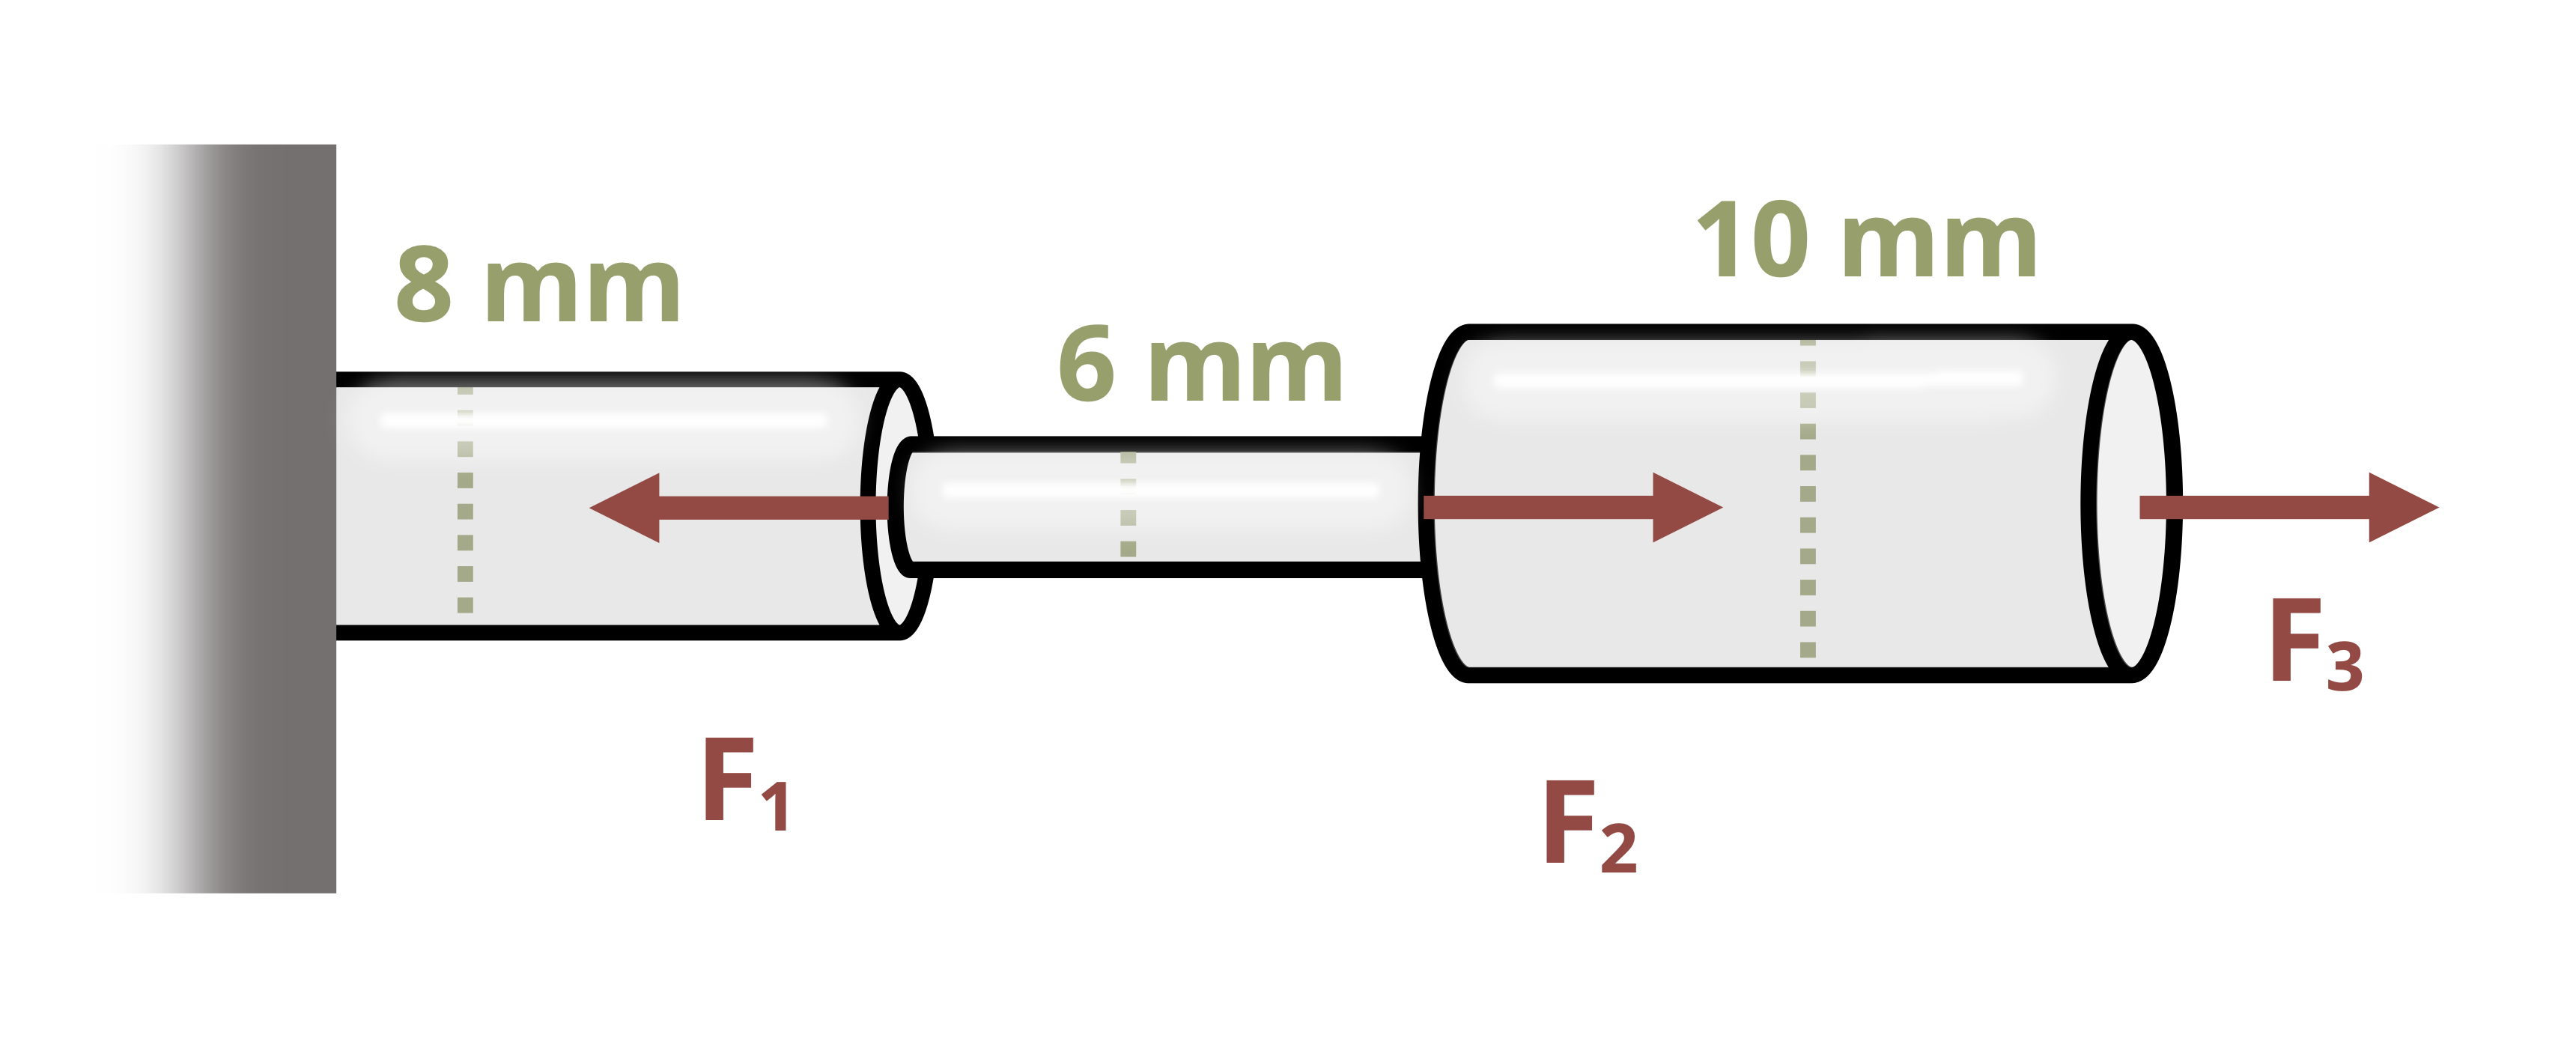
\includegraphics{images/138.png}

}

\caption{Figure 1: A series of solid circular bars are loaded with three
loads}

\end{figure}%

\begin{Shaded}
\begin{Highlighting}[]
\NormalTok{\#| standalone: true}
\NormalTok{\#| viewerHeight: 600}
\NormalTok{\#| components: [viewer]}

\NormalTok{from shiny import App, render, ui, reactive}
\NormalTok{import random}
\NormalTok{import asyncio}
\NormalTok{import io}
\NormalTok{import math}
\NormalTok{import string}
\NormalTok{from datetime import datetime}
\NormalTok{from pathlib import Path}


\NormalTok{def generate\_random\_letters(length):}
\NormalTok{    \# Generate a random string of letters of specified length}
\NormalTok{    return \textquotesingle{}\textquotesingle{}.join(random.choice(string.ascii\_lowercase) for \_ in range(length))  }

\NormalTok{problem\_ID="138"}
\NormalTok{F1=reactive.Value("\_\_")}
\NormalTok{F2=reactive.Value("\_\_")}
\NormalTok{F3=reactive.Value("\_\_")}
\NormalTok{d1=8}
\NormalTok{d2=6}
\NormalTok{d3=10}
\NormalTok{attempts=["Timestamp,Attempt,Answer,Feedback\textbackslash{}n"]}

\NormalTok{app\_ui = ui.page\_fluid(}
\NormalTok{    ui.markdown("**Please enter your ID number from your instructor and click to generate your problem**"),}
\NormalTok{    ui.input\_text("ID","", placeholder="Enter ID Number Here"),}
\NormalTok{    ui.input\_action\_button("generate\_problem", "Generate Problem", class\_="btn{-}primary"),}
\NormalTok{    ui.markdown("**Problem Statement**"),}
\NormalTok{    ui.output\_ui("ui\_problem\_statement"),}
\NormalTok{    ui.input\_text("answer","Your Answer in units of MPa", placeholder="Please enter your answer"),}
\NormalTok{    ui.input\_action\_button("submit", "Submit Answer", class\_="btn{-}primary"),}
\NormalTok{    ui.download\_button("download", "Download File to Submit", class\_="btn{-}success"),}
\NormalTok{)}


\NormalTok{def server(input, output, session):}
\NormalTok{    \# Initialize a counter for attempts}
\NormalTok{    attempt\_counter = reactive.Value(0)}
    
\NormalTok{    @output}
\NormalTok{    @render.ui}
\NormalTok{    def ui\_problem\_statement():}
\NormalTok{        return[ui.markdown(f"A series of solid circular bars are loaded with three loads as shown, F\textless{}sub\textgreater{}1\textless{}/sub\textgreater{} = \{F1()\} N, F\textless{}sub\textgreater{}2\textless{}/sub\textgreater{} = \{F2()\} N, and F\textless{}sub\textgreater{}3\textless{}/sub\textgreater{} = \{F3()\} N. What is the largest absolute normal stress in any bar?")]}
     
\NormalTok{    @reactive.Effect}
\NormalTok{    @reactive.event(input.generate\_problem)}
\NormalTok{    def randomize\_vars():}
\NormalTok{        random.seed(input.ID())}
\NormalTok{        F1.set(random.randrange(50, 70, 1))}
\NormalTok{        F2.set(random.randrange(10, 30, 1))}
\NormalTok{        F3.set(F1(){-}F2())}
        

\NormalTok{    @reactive.Effect}
\NormalTok{    @reactive.event(input.submit)}
\NormalTok{    def \_():}
\NormalTok{        attempt\_counter.set(attempt\_counter() + 1)  \# Increment the attempt counter on each submission.}
        
\NormalTok{        \# Calculate the instructor\textquotesingle{}s answer and determine if the user\textquotesingle{}s answer is correct.}
\NormalTok{        instr= (F1()/(math.pi*(d2/(1000*2))**2))/10**6}
        
\NormalTok{        if math.isclose(float(input.answer()), instr, rel\_tol=0.001):}
\NormalTok{            check = "*Correct*"}
\NormalTok{            correct\_indicator = "JL"}
\NormalTok{        else:}
\NormalTok{            check = "*Not Correct.*"}
\NormalTok{            correct\_indicator = "JG"}

\NormalTok{        \# Generate random parts for the encoded attempt.}
\NormalTok{        random\_start = generate\_random\_letters(4)}
\NormalTok{        random\_middle = generate\_random\_letters(4)}
\NormalTok{        random\_end = generate\_random\_letters(4)}
\NormalTok{        encoded\_attempt = f"\{random\_start\}\{problem\_ID\}{-}\{random\_middle\}\{attempt\_counter()\}\{correct\_indicator\}{-}\{random\_end\}\{input.ID()\}"}

\NormalTok{        \# Store the most recent encoded attempt in a reactive value so it persists across submissions}
\NormalTok{        session.encoded\_attempt = reactive.Value(encoded\_attempt)}

\NormalTok{        \# Append the attempt data to the attempts list without the encoded attempt}
\NormalTok{        attempts.append(f"\{datetime.now()\}, \{attempt\_counter()\}, \{input.answer()\}, \{check\}\textbackslash{}n")}

\NormalTok{        \# Show feedback to the user.}
\NormalTok{        feedback = ui.markdown(f"Your answer of \{input.answer()\} is \{check\}. For reference in debugging this, the calculated instructor answer is \{instr\}")}
\NormalTok{        m = ui.modal(}
\NormalTok{            feedback,}
\NormalTok{            title="Feedback",}
\NormalTok{            easy\_close=True}
\NormalTok{        )}
\NormalTok{        ui.modal\_show(m)}

\NormalTok{    @session.download(filename=lambda: f"Problem\_Log{-}\{problem\_ID\}{-}\{input.ID()\}.csv")}
\NormalTok{    async def download():}
\NormalTok{        \# Start the CSV with the encoded attempt (without label)}
\NormalTok{        final\_encoded = session.encoded\_attempt() if session.encoded\_attempt is not None else "No attempts"}
\NormalTok{        yield f"\{final\_encoded\}\textbackslash{}n\textbackslash{}n"}
        
\NormalTok{        \# Write the header for the remaining CSV data once}
\NormalTok{        yield "Timestamp,Attempt,Answer,Feedback\textbackslash{}n"}
        
\NormalTok{        \# Write the attempts data, ensure that the header from the attempts list is not written again}
\NormalTok{        for attempt in attempts[1:]:  \# Skip the first element which is the header}
\NormalTok{            await asyncio.sleep(0.25)  \# This delay may not be necessary; adjust as needed}
\NormalTok{            yield attempt}


\NormalTok{\# App installation}
\NormalTok{app = App(app\_ui, server)}
\end{Highlighting}
\end{Shaded}

\chapter*{Problem 2.2}\label{problem-2.2}
\addcontentsline{toc}{chapter}{Problem 2.2}

\markboth{Problem 2.2}{Problem 2.2}

This is a dynamic rendering of the problem with dynamic variables based
on the username entered.

\section*{Problem Image}\label{problem-image-2}
\addcontentsline{toc}{section}{Problem Image}

\markright{Problem Image}

\begin{figure}[H]

{\centering 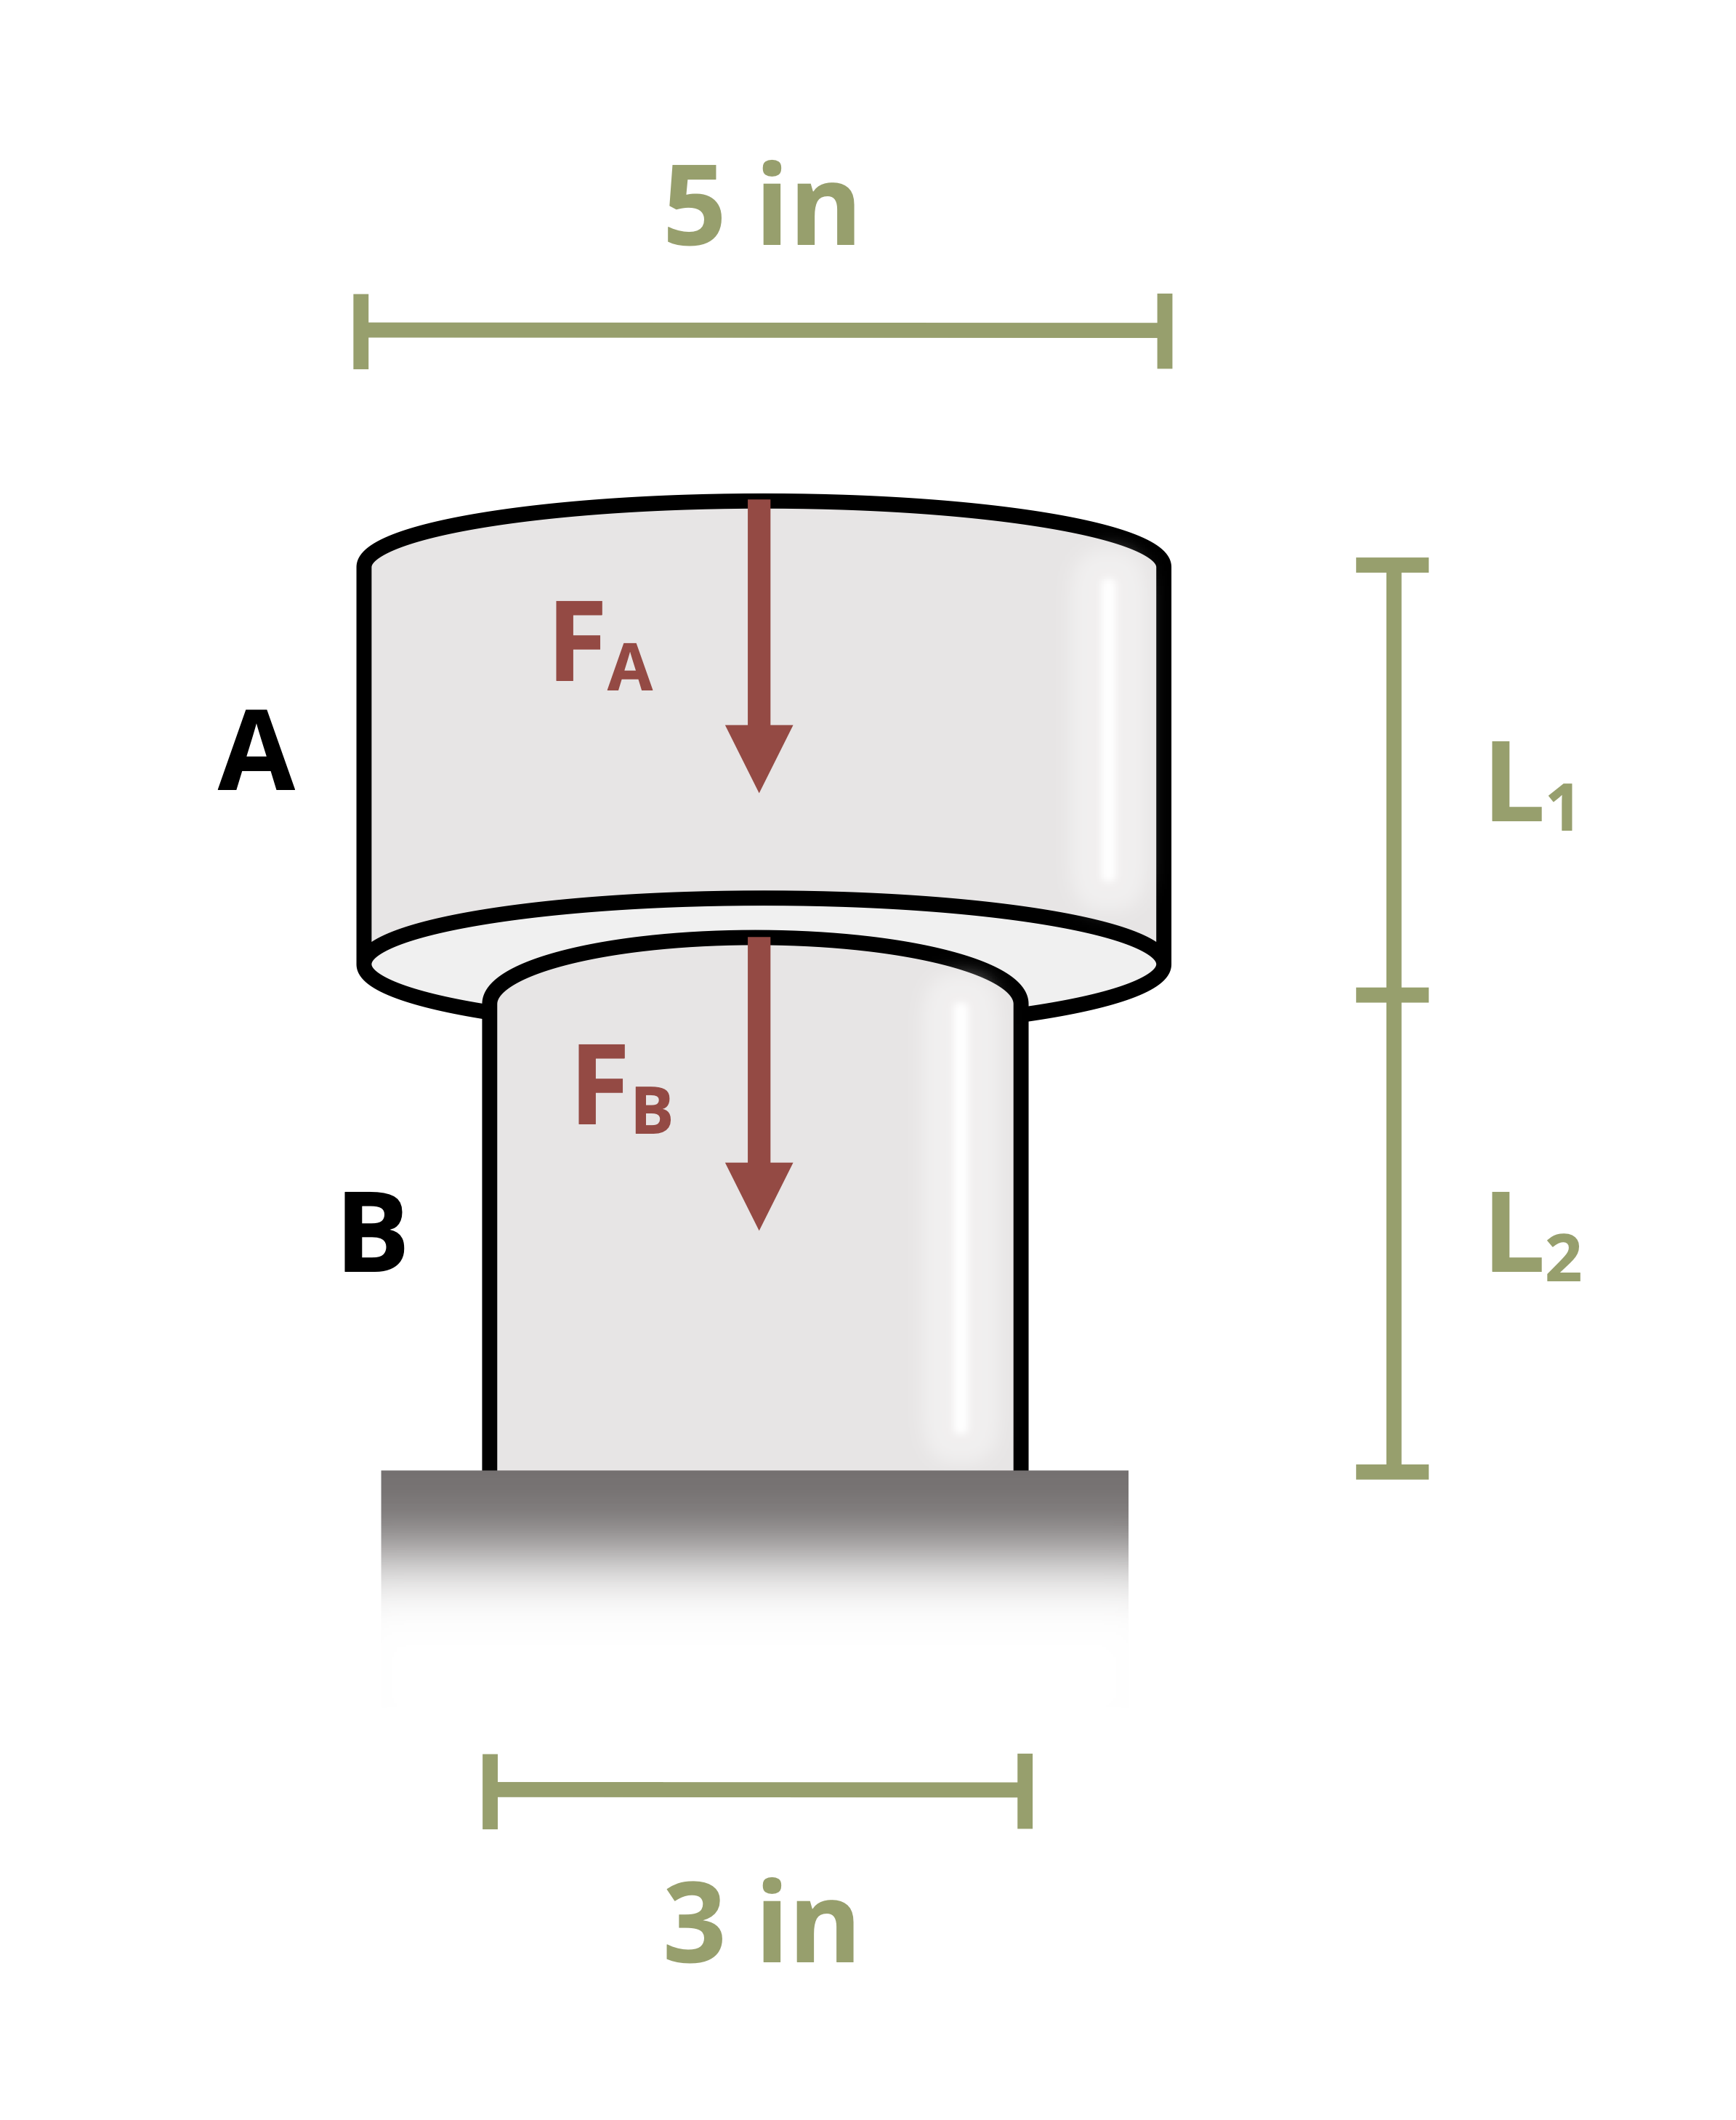
\includegraphics{images/139.png}

}

\caption{Figure 1: Two sylinders are stacked on top of each other.}

\end{figure}%

\begin{Shaded}
\begin{Highlighting}[]
\NormalTok{\#| standalone: true}
\NormalTok{\#| viewerHeight: 600}
\NormalTok{\#| components: [viewer]}

\NormalTok{from shiny import App, render, ui, reactive}
\NormalTok{import random}
\NormalTok{import asyncio}
\NormalTok{import io}
\NormalTok{import math}
\NormalTok{import string}
\NormalTok{from datetime import datetime}
\NormalTok{from pathlib import Path}

\NormalTok{def generate\_random\_letters(length):}
\NormalTok{    \# Generate a random string of letters of specified length}
\NormalTok{    return \textquotesingle{}\textquotesingle{}.join(random.choice(string.ascii\_lowercase) for \_ in range(length))  }

\NormalTok{problem\_ID="139"}
\NormalTok{L1=reactive.Value("\_\_")}
\NormalTok{L2=reactive.Value("\_\_")}
\NormalTok{FA=reactive.Value("\_\_")}
\NormalTok{FB=reactive.Value("\_\_")}
\NormalTok{E = 30*10**6}
  
\NormalTok{attempts=["Timestamp,Attempt,Answer,Feedback\textbackslash{}n"]}

\NormalTok{app\_ui = ui.page\_fluid(}
\NormalTok{    ui.markdown("**Please enter your ID number from your instructor and click to generate your problem**"),}
\NormalTok{    ui.input\_text("ID","", placeholder="Enter ID Number Here"),}
\NormalTok{    ui.input\_action\_button("generate\_problem", "Generate Problem", class\_="btn{-}primary"),}
\NormalTok{    ui.markdown("**Problem Statement**"),}
\NormalTok{    ui.output\_ui("ui\_problem\_statement"),}
\NormalTok{    ui.input\_text("answer","Your Answer in units of inches", placeholder="Please enter your answer"),}
\NormalTok{    ui.input\_action\_button("submit", "Submit Answer", class\_="btn{-}primary"),}
\NormalTok{    ui.download\_button("download", "Download File to Submit", class\_="btn{-}success"),}
\NormalTok{)}


\NormalTok{def server(input, output, session):}
\NormalTok{    \# Initialize a counter for attempts}
\NormalTok{    attempt\_counter = reactive.Value(0)}

\NormalTok{    @output}
\NormalTok{    @render.ui}
\NormalTok{    def ui\_problem\_statement():}
\NormalTok{        return[ui.markdown(f"Two cylinders are stacked on top of one another and two forces are applied at the top surface and at the joint between the cylinders as shown. If L\textless{}sub\textgreater{}1\textless{}/sub\textgreater{} = \{L1()\} in., L\textless{}sub\textgreater{}2\textless{}/sub\textgreater{} = \{L2()\} in., F\textless{}sub\textgreater{}A\textless{}/sub\textgreater{} = \{FA()\} lb, and F\textless{}sub\textgreater{}B\textless{}/sub\textgreater{} = \{FB()\} lb, find the total deflection in the stack of cylinders. Assume E = 30 x 10\textless{}sup\textgreater{}6\textless{}/sup\textgreater{} psi for both cylinders. ")]}
    
\NormalTok{    @reactive.Effect}
\NormalTok{    @reactive.event(input.generate\_problem)}
\NormalTok{    def randomize\_vars():}
\NormalTok{        random.seed(input.ID())}
\NormalTok{        FA.set(random.randrange(300, 700, 10))}
\NormalTok{        FB.set(random.randrange(100, 300, 10))}
\NormalTok{        L1.set(random.randrange(2, 7, 1))}
\NormalTok{        L2.set(L1() * 1.3)}
        

\NormalTok{    @reactive.Effect}
\NormalTok{    @reactive.event(input.submit)}
\NormalTok{    def \_():}
\NormalTok{        attempt\_counter.set(attempt\_counter() + 1)  \# Increment the attempt counter on each submission.}
    
\NormalTok{        instr= (FA()*L1())/((math.pi*(5/2)**2)*E) + (FB()*L2())/((math.pi*(3/2)**2)*E)}
\NormalTok{        if math.isclose(float(input.answer()), instr, rel\_tol=0.001):}
\NormalTok{            check = "*Correct*"}
\NormalTok{            correct\_indicator = "JL"}
\NormalTok{        else:}
\NormalTok{            check = "*Not Correct.*"}
\NormalTok{            correct\_indicator = "JG"}

\NormalTok{        \# Generate random parts for the encoded attempt.}
\NormalTok{        random\_start = generate\_random\_letters(4)}
\NormalTok{        random\_middle = generate\_random\_letters(4)}
\NormalTok{        random\_end = generate\_random\_letters(4)}
\NormalTok{        encoded\_attempt = f"\{random\_start\}\{problem\_ID\}{-}\{random\_middle\}\{attempt\_counter()\}\{correct\_indicator\}{-}\{random\_end\}\{input.ID()\}"}

\NormalTok{        \# Store the most recent encoded attempt in a reactive value so it persists across submissions}
\NormalTok{        session.encoded\_attempt = reactive.Value(encoded\_attempt)}

\NormalTok{        \# Append the attempt data to the attempts list without the encoded attempt}
\NormalTok{        attempts.append(f"\{datetime.now()\}, \{attempt\_counter()\}, \{input.answer()\}, \{check\}\textbackslash{}n")}

\NormalTok{        \# Show feedback to the user.}
\NormalTok{        feedback = ui.markdown(f"Your answer of \{input.answer()\} is \{check\}. For reference in debugging this, the calculated instructor answer is \{instr\}")}
\NormalTok{        m = ui.modal(}
\NormalTok{            feedback,}
\NormalTok{            title="Feedback",}
\NormalTok{            easy\_close=True}
\NormalTok{        )}
\NormalTok{        ui.modal\_show(m)}

\NormalTok{    @session.download(filename=lambda: f"Problem\_Log{-}\{problem\_ID\}{-}\{input.ID()\}.csv")}
\NormalTok{    async def download():}
\NormalTok{        \# Start the CSV with the encoded attempt (without label)}
\NormalTok{        final\_encoded = session.encoded\_attempt() if session.encoded\_attempt is not None else "No attempts"}
\NormalTok{        yield f"\{final\_encoded\}\textbackslash{}n\textbackslash{}n"}
        
\NormalTok{        \# Write the header for the remaining CSV data once}
\NormalTok{        yield "Timestamp,Attempt,Answer,Feedback\textbackslash{}n"}
        
\NormalTok{        \# Write the attempts data, ensure that the header from the attempts list is not written again}
\NormalTok{        for attempt in attempts[1:]:  \# Skip the first element which is the header}
\NormalTok{            await asyncio.sleep(0.25)  \# This delay may not be necessary; adjust as needed}
\NormalTok{            yield attempt}


\NormalTok{\# App installation}
\NormalTok{app = App(app\_ui, server)}
\end{Highlighting}
\end{Shaded}

\chapter*{Problem 2.3}\label{problem-2.3}
\addcontentsline{toc}{chapter}{Problem 2.3}

\markboth{Problem 2.3}{Problem 2.3}

This is a dynamic rendering of the problem with dynamic variables based
on the username entered.

\section*{Problem Image}\label{problem-image-3}
\addcontentsline{toc}{section}{Problem Image}

\markright{Problem Image}

\begin{figure}[H]

{\centering 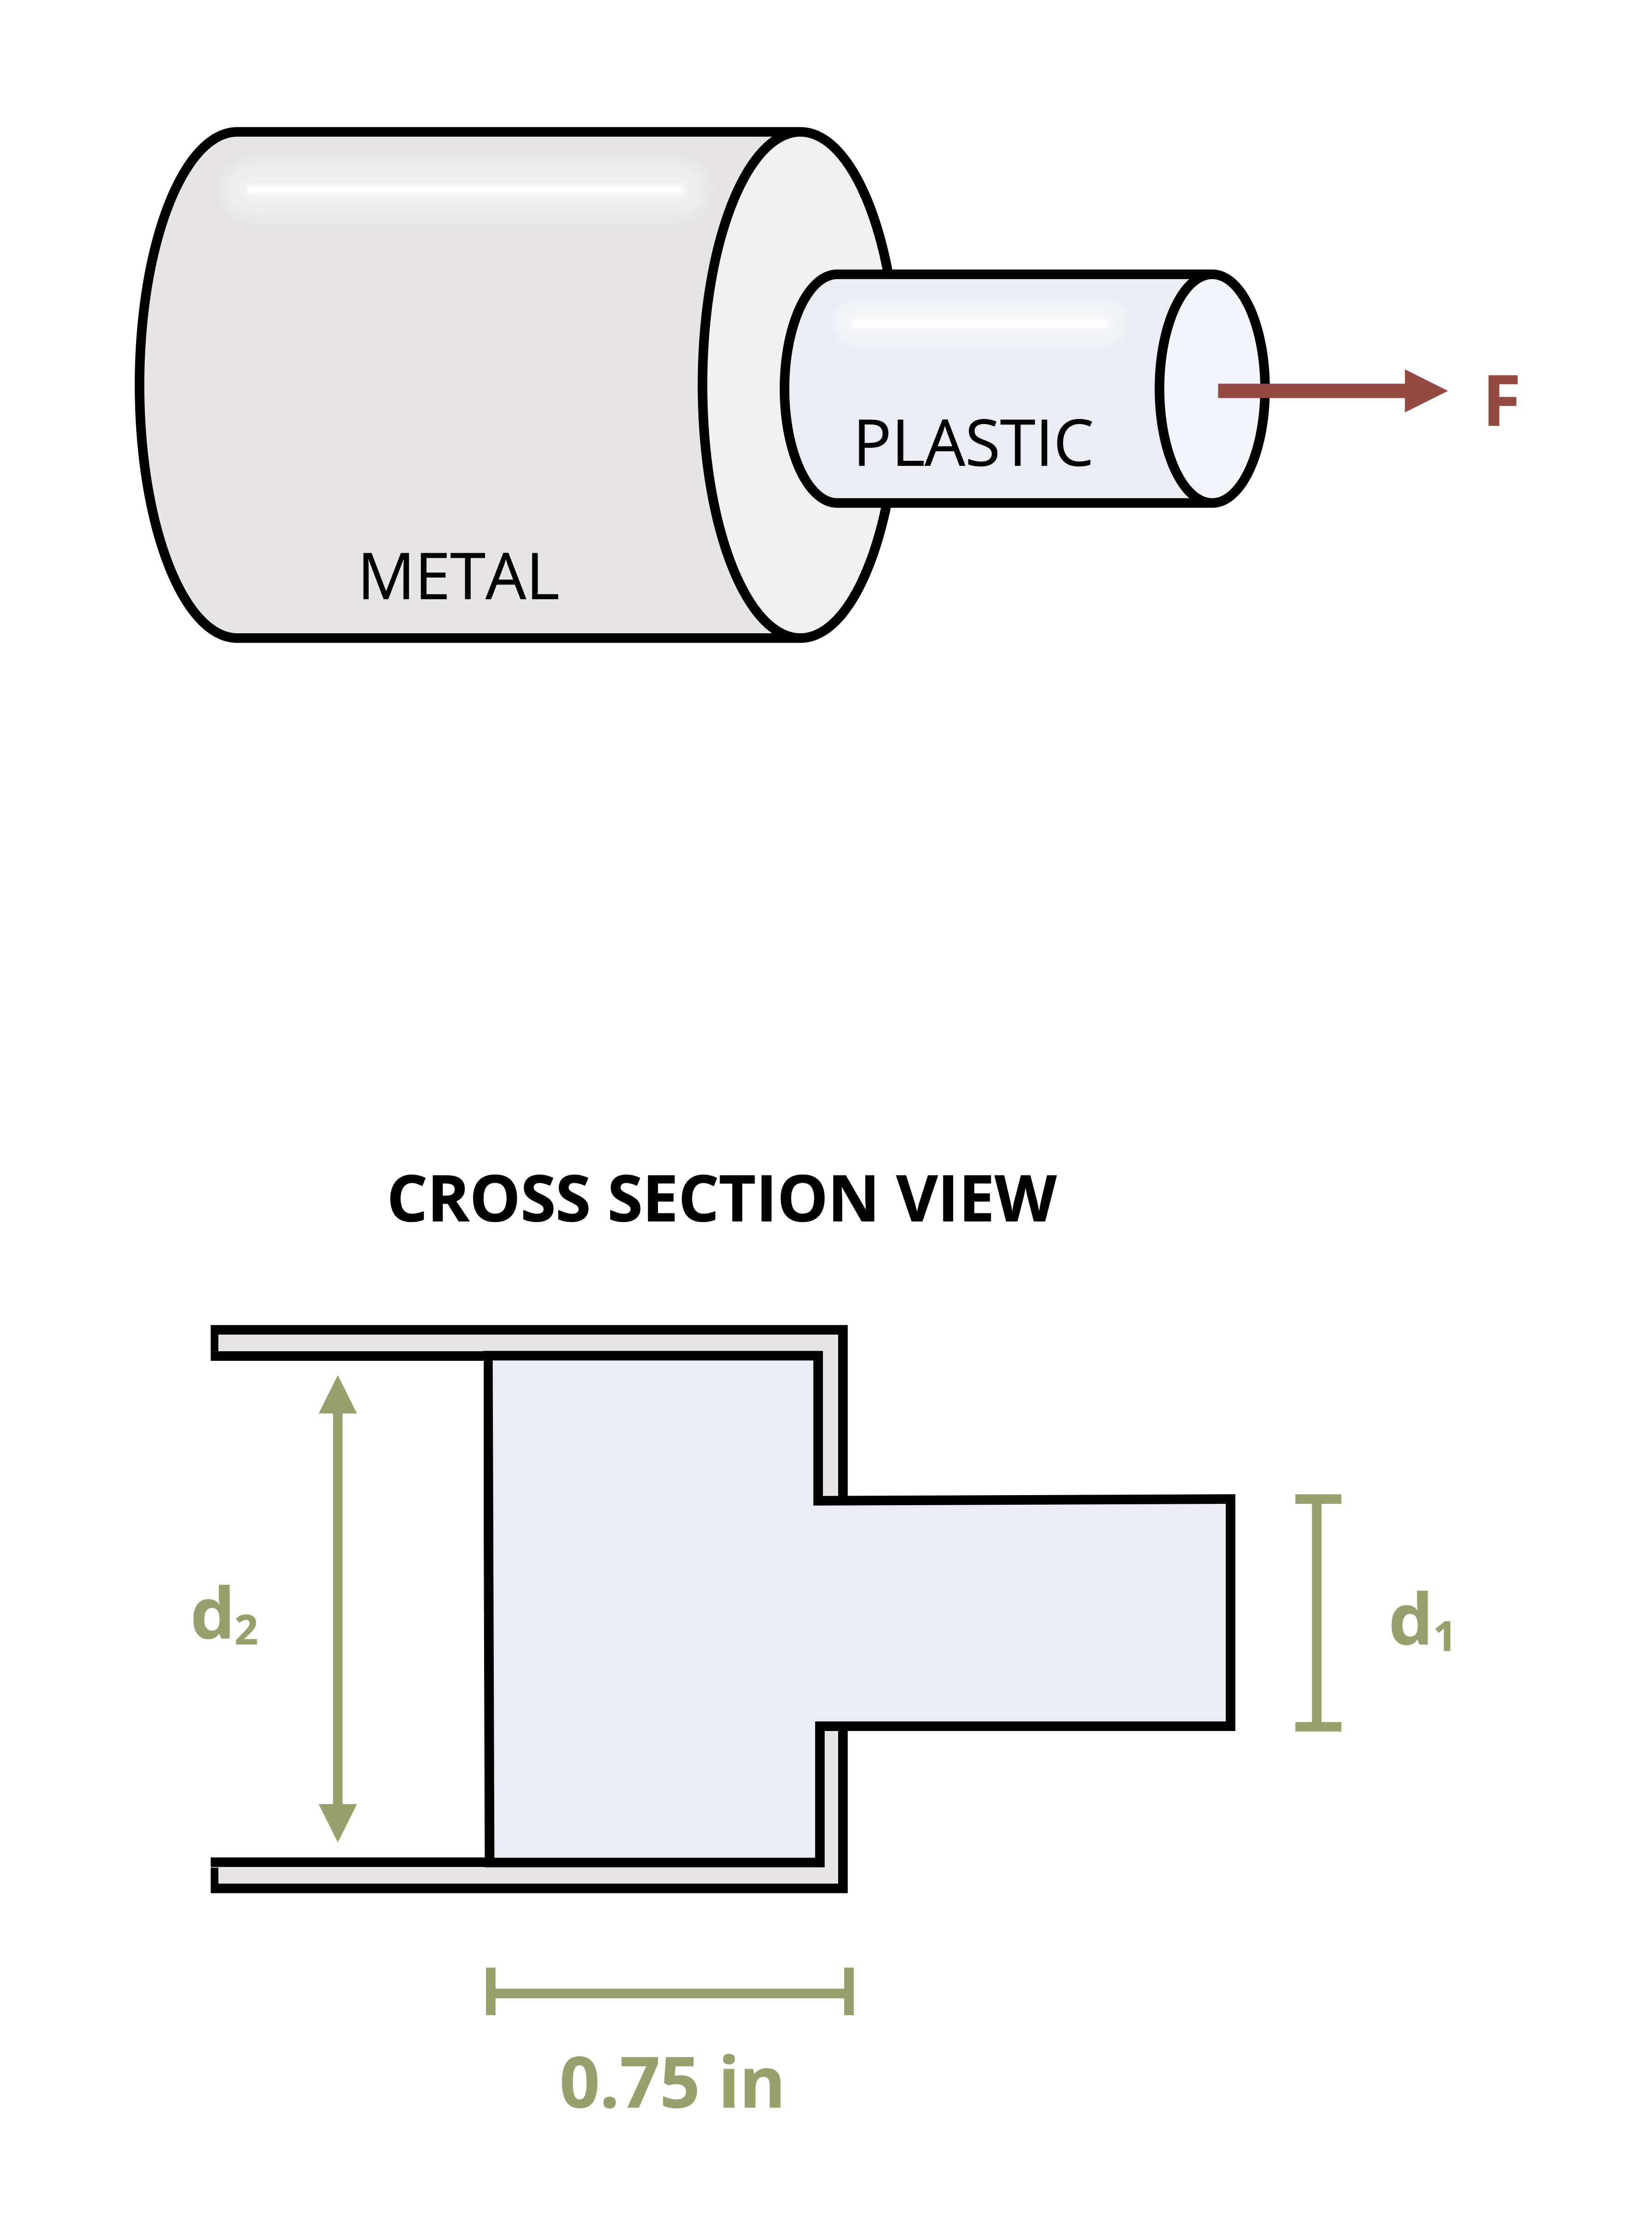
\includegraphics{images/144.png}

}

\caption{Figure 1: A plastic cylindrical peg is constrained by a metal
cap}

\end{figure}%

\begin{Shaded}
\begin{Highlighting}[]
\NormalTok{\#| standalone: true}
\NormalTok{\#| viewerHeight: 600}
\NormalTok{\#| components: [viewer]}

\NormalTok{from shiny import App, render, ui, reactive}
\NormalTok{import random}
\NormalTok{import asyncio}
\NormalTok{import io}
\NormalTok{import math}
\NormalTok{import string}
\NormalTok{from datetime import datetime}
\NormalTok{from pathlib import Path}

\NormalTok{def generate\_random\_letters(length):}
\NormalTok{    \# Generate a random string of letters of specified length}
\NormalTok{    return \textquotesingle{}\textquotesingle{}.join(random.choice(string.ascii\_lowercase) for \_ in range(length))}

\NormalTok{problem\_ID="144"}
\NormalTok{F=reactive.Value("\_\_")}
\NormalTok{d1=reactive.Value("\_\_")}
\NormalTok{d2=reactive.Value("\_\_")}

\NormalTok{attempts=["Timestamp,Attempt,Answer,Feedback\textbackslash{}n"]}

\NormalTok{app\_ui = ui.page\_fluid(}
\NormalTok{    ui.markdown("**Please enter your ID number from your instructor and click to generate your problem**"),}
\NormalTok{    ui.input\_text("ID","", placeholder="Enter ID Number Here"),}
\NormalTok{    ui.input\_action\_button("generate\_problem", "Generate Problem", class\_="btn{-}primary"),}
\NormalTok{    ui.markdown("**Problem Statement**"),}
\NormalTok{    ui.output\_ui("ui\_problem\_statement"),}
\NormalTok{    ui.input\_text("answer","Your Answer in units of psi", placeholder="Please enter your answer"),}
\NormalTok{    ui.input\_action\_button("submit", "Submit Answer", class\_="btn{-}primary"),}
\NormalTok{    ui.download\_button("download", "Download File to Submit", class\_="btn{-}success"),}
\NormalTok{)}


\NormalTok{def server(input, output, session):}
\NormalTok{    \# Initialize a counter for attempts}
\NormalTok{    attempt\_counter = reactive.Value(0)}

\NormalTok{    @output}
\NormalTok{    @render.ui}
\NormalTok{    def ui\_problem\_statement():}
\NormalTok{        return[ui.markdown(f"A plastic cylindrical peg is constrained by a metal cap as shown. An axial load of F = \{F()\} lb is applied to the peg. If d\textless{}sub\textgreater{}1\textless{}/sub\textgreater{} = \{d1()\} in and d\textless{}sub\textgreater{}2\textless{}/sub\textgreater{} = \{d2()\} in, determine the normal stress in the peg. Assume the axial load is evenly distributed across the peg and that the metal cap is fixed and does not move.")]}
    
\NormalTok{    @reactive.Effect}
\NormalTok{    @reactive.event(input.generate\_problem)}
\NormalTok{    def randomize\_vars():}
\NormalTok{        random.seed(input.ID())}
\NormalTok{        F.set(random.randrange(20, 80, 5))}
\NormalTok{        d1.set(random.randrange(3, 8, 1)/10)}
\NormalTok{        d2.set(round(d1() * 1.6, 2))}
        
 
\NormalTok{    @reactive.Effect}
\NormalTok{    @reactive.event(input.submit)}
\NormalTok{    def \_():}
\NormalTok{        attempt\_counter.set(attempt\_counter() + 1)  \# Increment the attempt counter on each submission.}
\NormalTok{        instr= F()/(math.pi*((d1()/2)**2))}
\NormalTok{        \#check=math.isclose(float(input.answer()),instr,rel\_tol=0.001)}
        
\NormalTok{        if math.isclose(float(input.answer()), instr, rel\_tol=0.001):}
\NormalTok{            check = "*Correct*"}
\NormalTok{            correct\_indicator = "JL"}
\NormalTok{        else:}
\NormalTok{            check = "*Not Correct.*"}
\NormalTok{            correct\_indicator = "JG"}

\NormalTok{        \# Generate random parts for the encoded attempt.}
\NormalTok{        random\_start = generate\_random\_letters(4)}
\NormalTok{        random\_middle = generate\_random\_letters(4)}
\NormalTok{        random\_end = generate\_random\_letters(4)}
\NormalTok{        encoded\_attempt = f"\{random\_start\}\{problem\_ID\}{-}\{random\_middle\}\{attempt\_counter()\}\{correct\_indicator\}{-}\{random\_end\}\{input.ID()\}"}

\NormalTok{        \# Store the most recent encoded attempt in a reactive value so it persists across submissions}
\NormalTok{        session.encoded\_attempt = reactive.Value(encoded\_attempt)}

\NormalTok{        \# Append the attempt data to the attempts list without the encoded attempt}
\NormalTok{        attempts.append(f"\{datetime.now()\}, \{attempt\_counter()\}, \{input.answer()\}, \{check\}\textbackslash{}n")}

\NormalTok{        \# Show feedback to the user.}
\NormalTok{        feedback = ui.markdown(f"Your answer of \{input.answer()\} is \{check\}. For reference in debugging this, the calculated instructor answer is \{instr\}")}
\NormalTok{        m = ui.modal(}
\NormalTok{            feedback,}
\NormalTok{            title="Feedback",}
\NormalTok{            easy\_close=True}
\NormalTok{        )}
\NormalTok{        ui.modal\_show(m)}

\NormalTok{    @session.download(filename=lambda: f"Problem\_Log{-}\{problem\_ID\}{-}\{input.ID()\}.csv")}
\NormalTok{    async def download():}
\NormalTok{        \# Start the CSV with the encoded attempt (without label)}
\NormalTok{        final\_encoded = session.encoded\_attempt() if session.encoded\_attempt is not None else "No attempts"}
\NormalTok{        yield f"\{final\_encoded\}\textbackslash{}n\textbackslash{}n"}
        
\NormalTok{        \# Write the header for the remaining CSV data once}
\NormalTok{        yield "Timestamp,Attempt,Answer,Feedback\textbackslash{}n"}
        
\NormalTok{        \# Write the attempts data, ensure that the header from the attempts list is not written again}
\NormalTok{        for attempt in attempts[1:]:  \# Skip the first element which is the header}
\NormalTok{            await asyncio.sleep(0.25)  \# This delay may not be necessary; adjust as needed}
\NormalTok{            yield attempt}


\NormalTok{\# App installation}
\NormalTok{app = App(app\_ui, server)}
\end{Highlighting}
\end{Shaded}

\chapter*{Problem 2.4}\label{problem-2.4}
\addcontentsline{toc}{chapter}{Problem 2.4}

\markboth{Problem 2.4}{Problem 2.4}

This is a dynamic rendering of the problem with dynamic variables based
on the username entered.

\section*{Problem Image}\label{problem-image-4}
\addcontentsline{toc}{section}{Problem Image}

\markright{Problem Image}

\begin{figure}[H]

{\centering 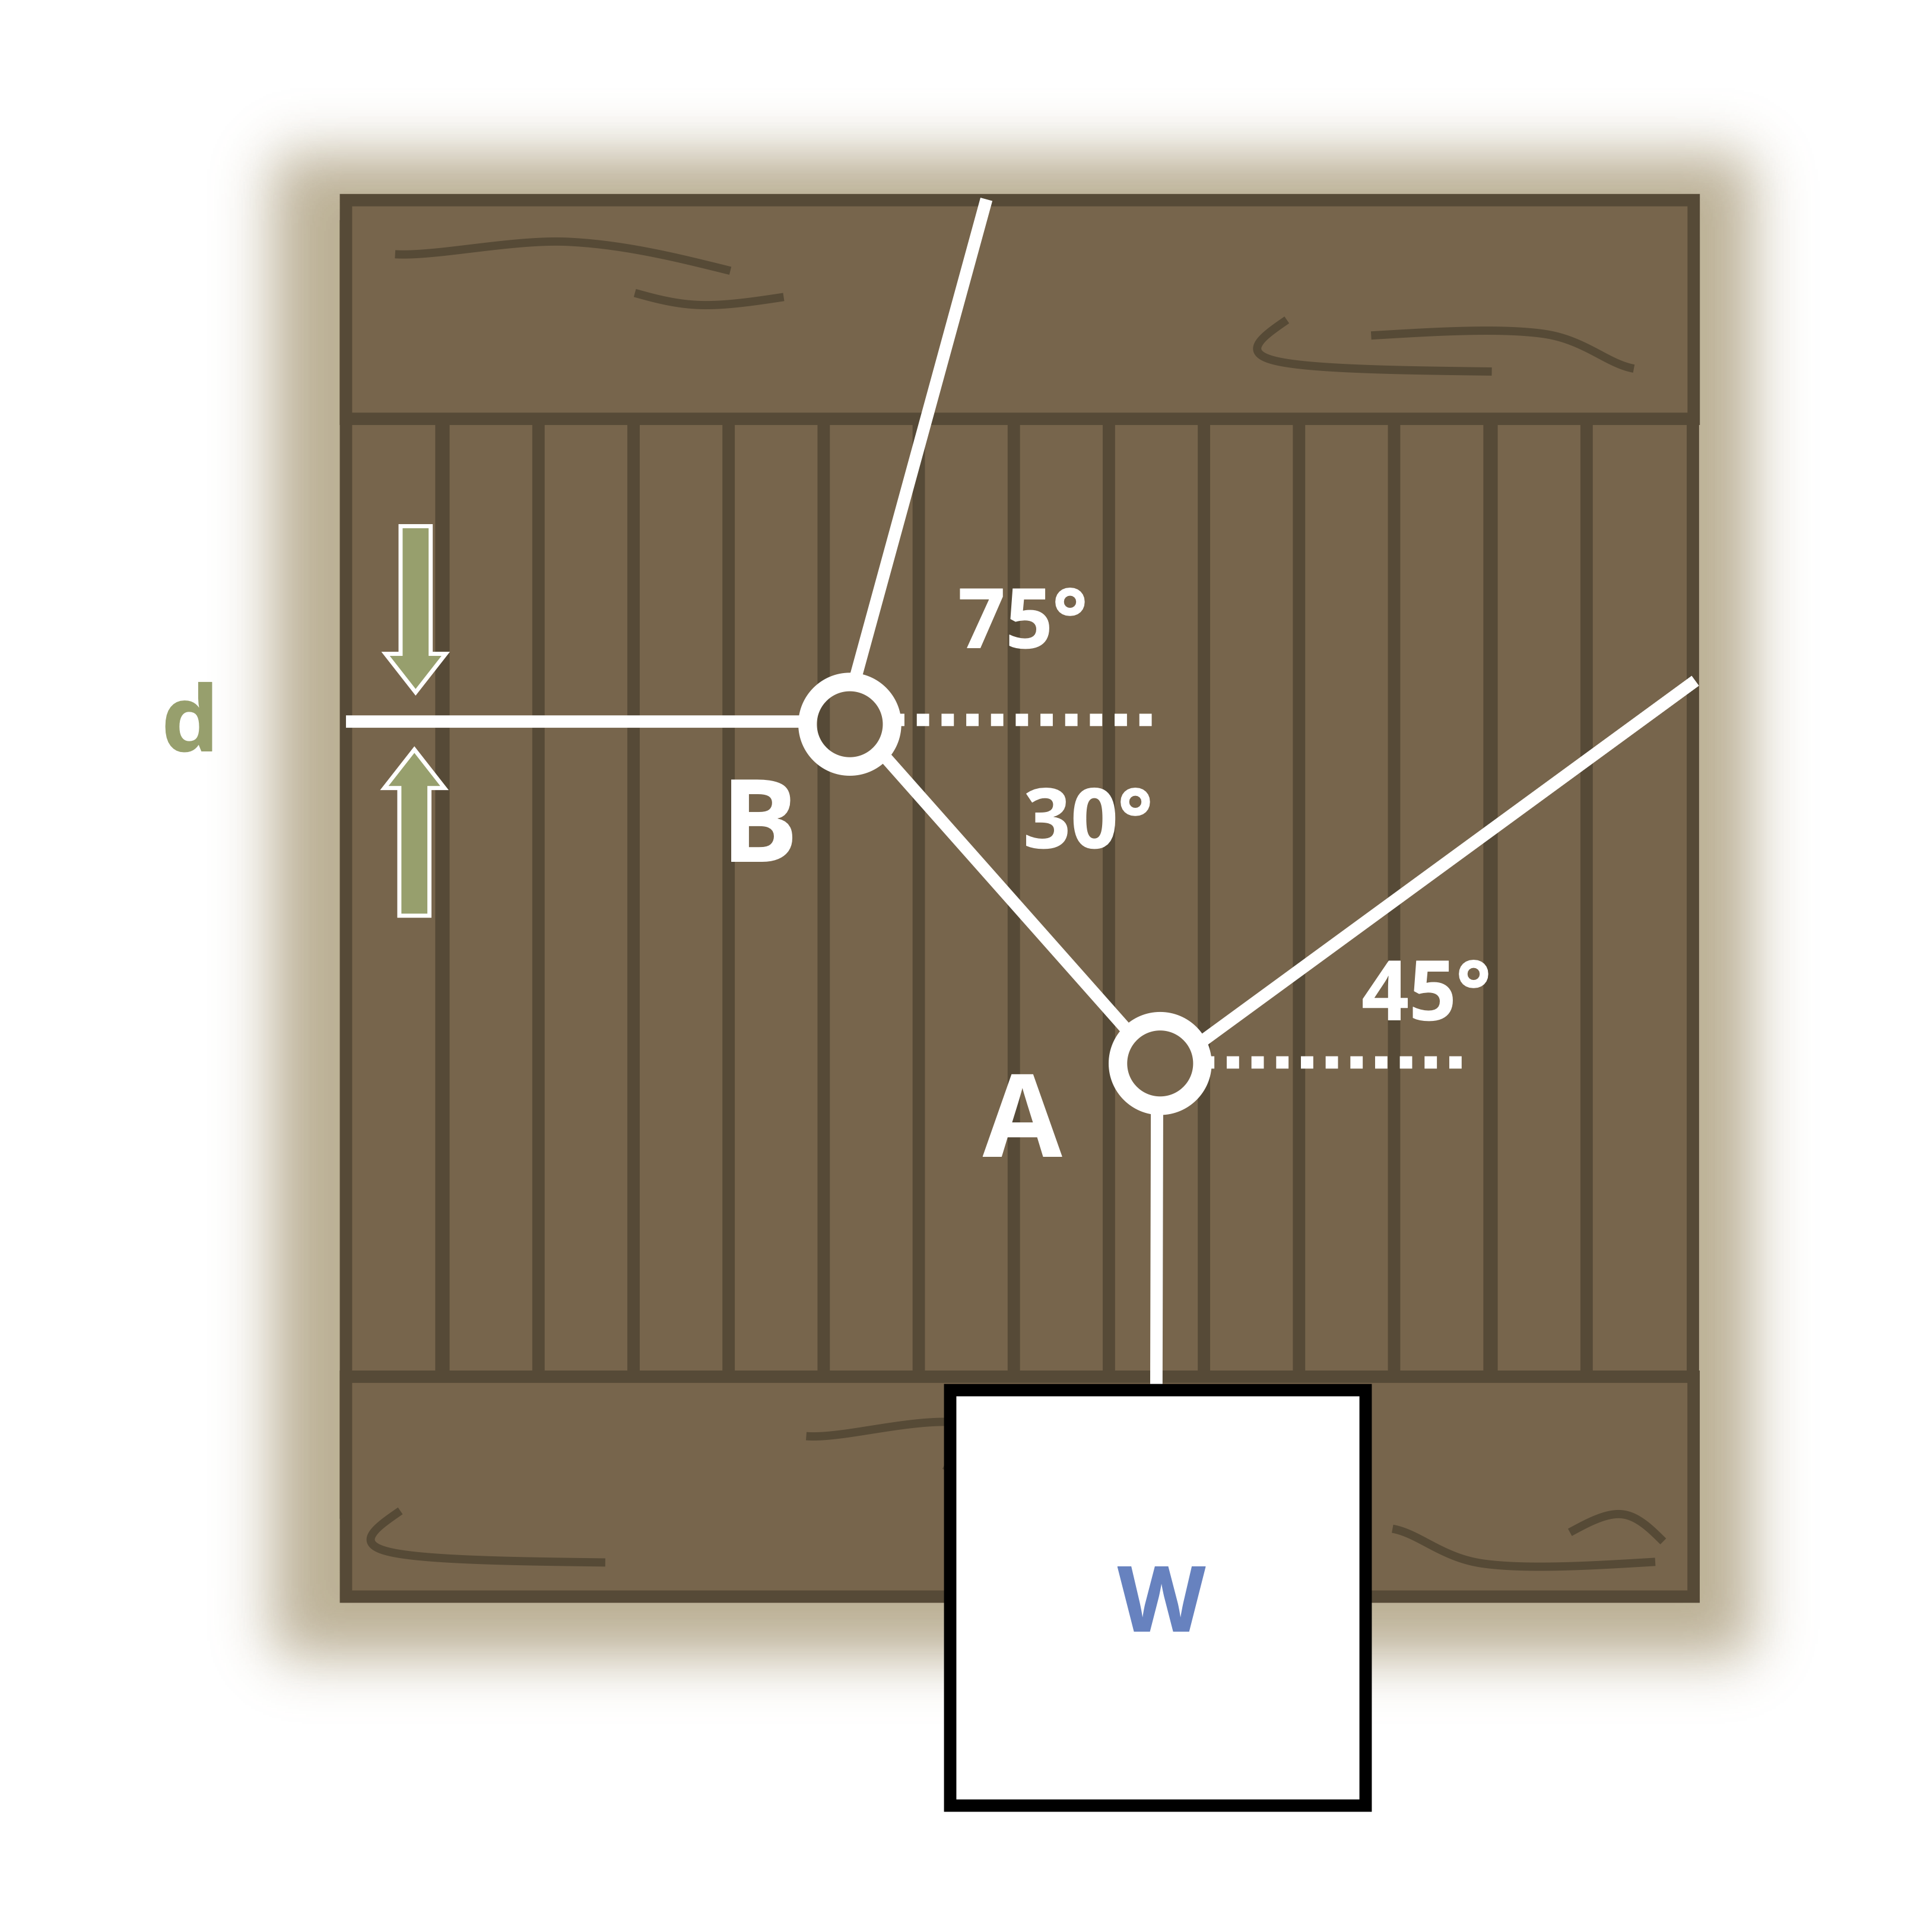
\includegraphics{images/146.png}

}

\caption{Figure 1: A crate is suspended by a set of cables}

\end{figure}%

\begin{Shaded}
\begin{Highlighting}[]
\NormalTok{\#| standalone: true}
\NormalTok{\#| viewerHeight: 600}
\NormalTok{\#| components: [viewer]}

\NormalTok{from shiny import App, render, ui, reactive}
\NormalTok{import random}
\NormalTok{import asyncio}
\NormalTok{import io}
\NormalTok{import math}
\NormalTok{import string}
\NormalTok{from datetime import datetime}
\NormalTok{from pathlib import Path}


\NormalTok{def generate\_random\_letters(length):}
\NormalTok{    \# Generate a random string of letters of specified length}
\NormalTok{    return \textquotesingle{}\textquotesingle{}.join(random.choice(string.ascii\_lowercase) for \_ in range(length)) }

\NormalTok{problem\_ID="146"}
\NormalTok{W=reactive.Value("\_\_")}
\NormalTok{d=reactive.Value("\_\_")}
\NormalTok{angle1=math.radians(45)}
\NormalTok{angle2=math.radians(30)}
\NormalTok{angle3=math.radians(75)}

\NormalTok{attempts=["Timestamp,Attempt,Answer,Feedback\textbackslash{}n"]}

\NormalTok{app\_ui = ui.page\_fluid(}
\NormalTok{    ui.markdown("**Please enter your ID number from your instructor and click to generate your problem**"),}
\NormalTok{    ui.input\_text("ID","", placeholder="Enter ID Number Here"),}
\NormalTok{    ui.input\_action\_button("generate\_problem", "Generate Problem", class\_="btn{-}primary"),}
\NormalTok{    ui.markdown("**Problem Statement**"),}
\NormalTok{    ui.output\_ui("ui\_problem\_statement"),}
\NormalTok{    ui.input\_text("answer","Your Answer in units of GPa", placeholder="Please enter your answer"),}
\NormalTok{    ui.input\_action\_button("submit", "Submit Answer", class\_="btn{-}primary"),}
\NormalTok{    ui.download\_button("download", "Download File to Submit", class\_="btn{-}success"),}
\NormalTok{)}


\NormalTok{def server(input, output, session):}
\NormalTok{    \# Initialize a counter for attempts}
\NormalTok{    attempt\_counter = reactive.Value(0)}

\NormalTok{    @output}
\NormalTok{    @render.ui}
\NormalTok{    def ui\_problem\_statement():}
\NormalTok{        return[ui.markdown(f"A crate weighing \{W()\} kN is suspended by a set of cables. The diameter of each cable is \{d()\}  mm. What is the maximum stress in any cable, exluding the cable attached to the crate.")]}
    
\NormalTok{    @reactive.Effect}
\NormalTok{    @reactive.event(input.generate\_problem)}
\NormalTok{    def randomize\_vars():}
\NormalTok{        random.seed(input.ID())}
\NormalTok{        W.set(random.randrange(30, 90, 1))}
\NormalTok{        d.set(random.randrange(20, 90, 1)/10)}
        

\NormalTok{    @reactive.Effect}
\NormalTok{    @reactive.event(input.submit)}
\NormalTok{    def \_():}
\NormalTok{        attempt\_counter.set(attempt\_counter() + 1)  \# Increment the attempt counter on each submission.}
    
\NormalTok{        R1 = W()/(((math.cos(angle1)/math.cos(angle2))*math.sin(angle2))+math.sin(angle1))}
\NormalTok{        instr= (R1*10**3/(math.pi*((d()/(1000*2))**2)))/10**9}
\NormalTok{        if math.isclose(float(input.answer()), instr, rel\_tol=0.001):}
\NormalTok{            check = "*Correct*"}
\NormalTok{            correct\_indicator = "JL"}
\NormalTok{        else:}
\NormalTok{            check = "*Not Correct.*"}
\NormalTok{            correct\_indicator = "JG"}

\NormalTok{        \# Generate random parts for the encoded attempt.}
\NormalTok{        random\_start = generate\_random\_letters(4)}
\NormalTok{        random\_middle = generate\_random\_letters(4)}
\NormalTok{        random\_end = generate\_random\_letters(4)}
\NormalTok{        encoded\_attempt = f"\{random\_start\}\{problem\_ID\}{-}\{random\_middle\}\{attempt\_counter()\}\{correct\_indicator\}{-}\{random\_end\}\{input.ID()\}"}

\NormalTok{        \# Store the most recent encoded attempt in a reactive value so it persists across submissions}
\NormalTok{        session.encoded\_attempt = reactive.Value(encoded\_attempt)}

\NormalTok{        \# Append the attempt data to the attempts list without the encoded attempt}
\NormalTok{        attempts.append(f"\{datetime.now()\}, \{attempt\_counter()\}, \{input.answer()\}, \{check\}\textbackslash{}n")}

\NormalTok{        \# Show feedback to the user.}
\NormalTok{        feedback = ui.markdown(f"Your answer of \{input.answer()\} is \{check\}. For reference in debugging this, the calculated instructor answer is \{instr\}")}
\NormalTok{        m = ui.modal(}
\NormalTok{            feedback,}
\NormalTok{            title="Feedback",}
\NormalTok{            easy\_close=True}
\NormalTok{        )}
\NormalTok{        ui.modal\_show(m)}

\NormalTok{    @session.download(filename=lambda: f"Problem\_Log{-}\{problem\_ID\}{-}\{input.ID()\}.csv")}
\NormalTok{    async def download():}
\NormalTok{        \# Start the CSV with the encoded attempt (without label)}
\NormalTok{        final\_encoded = session.encoded\_attempt() if session.encoded\_attempt is not None else "No attempts"}
\NormalTok{        yield f"\{final\_encoded\}\textbackslash{}n\textbackslash{}n"}
        
\NormalTok{        \# Write the header for the remaining CSV data once}
\NormalTok{        yield "Timestamp,Attempt,Answer,Feedback\textbackslash{}n"}
        
\NormalTok{        \# Write the attempts data, ensure that the header from the attempts list is not written again}
\NormalTok{        for attempt in attempts[1:]:  \# Skip the first element which is the header}
\NormalTok{            await asyncio.sleep(0.25)  \# This delay may not be necessary; adjust as needed}
\NormalTok{            yield attempt}


\NormalTok{\# App installation}
\NormalTok{app = App(app\_ui, server)}
\end{Highlighting}
\end{Shaded}

\chapter*{Problem 2.47}\label{problem-2.47}
\addcontentsline{toc}{chapter}{Problem 2.47}

\markboth{Problem 2.47}{Problem 2.47}

This is a dynamic rendering of the problem with dynamic variables based
on the username entered.

\section*{Problem Image}\label{problem-image-5}
\addcontentsline{toc}{section}{Problem Image}

\markright{Problem Image}

\begin{figure}[H]

{\centering 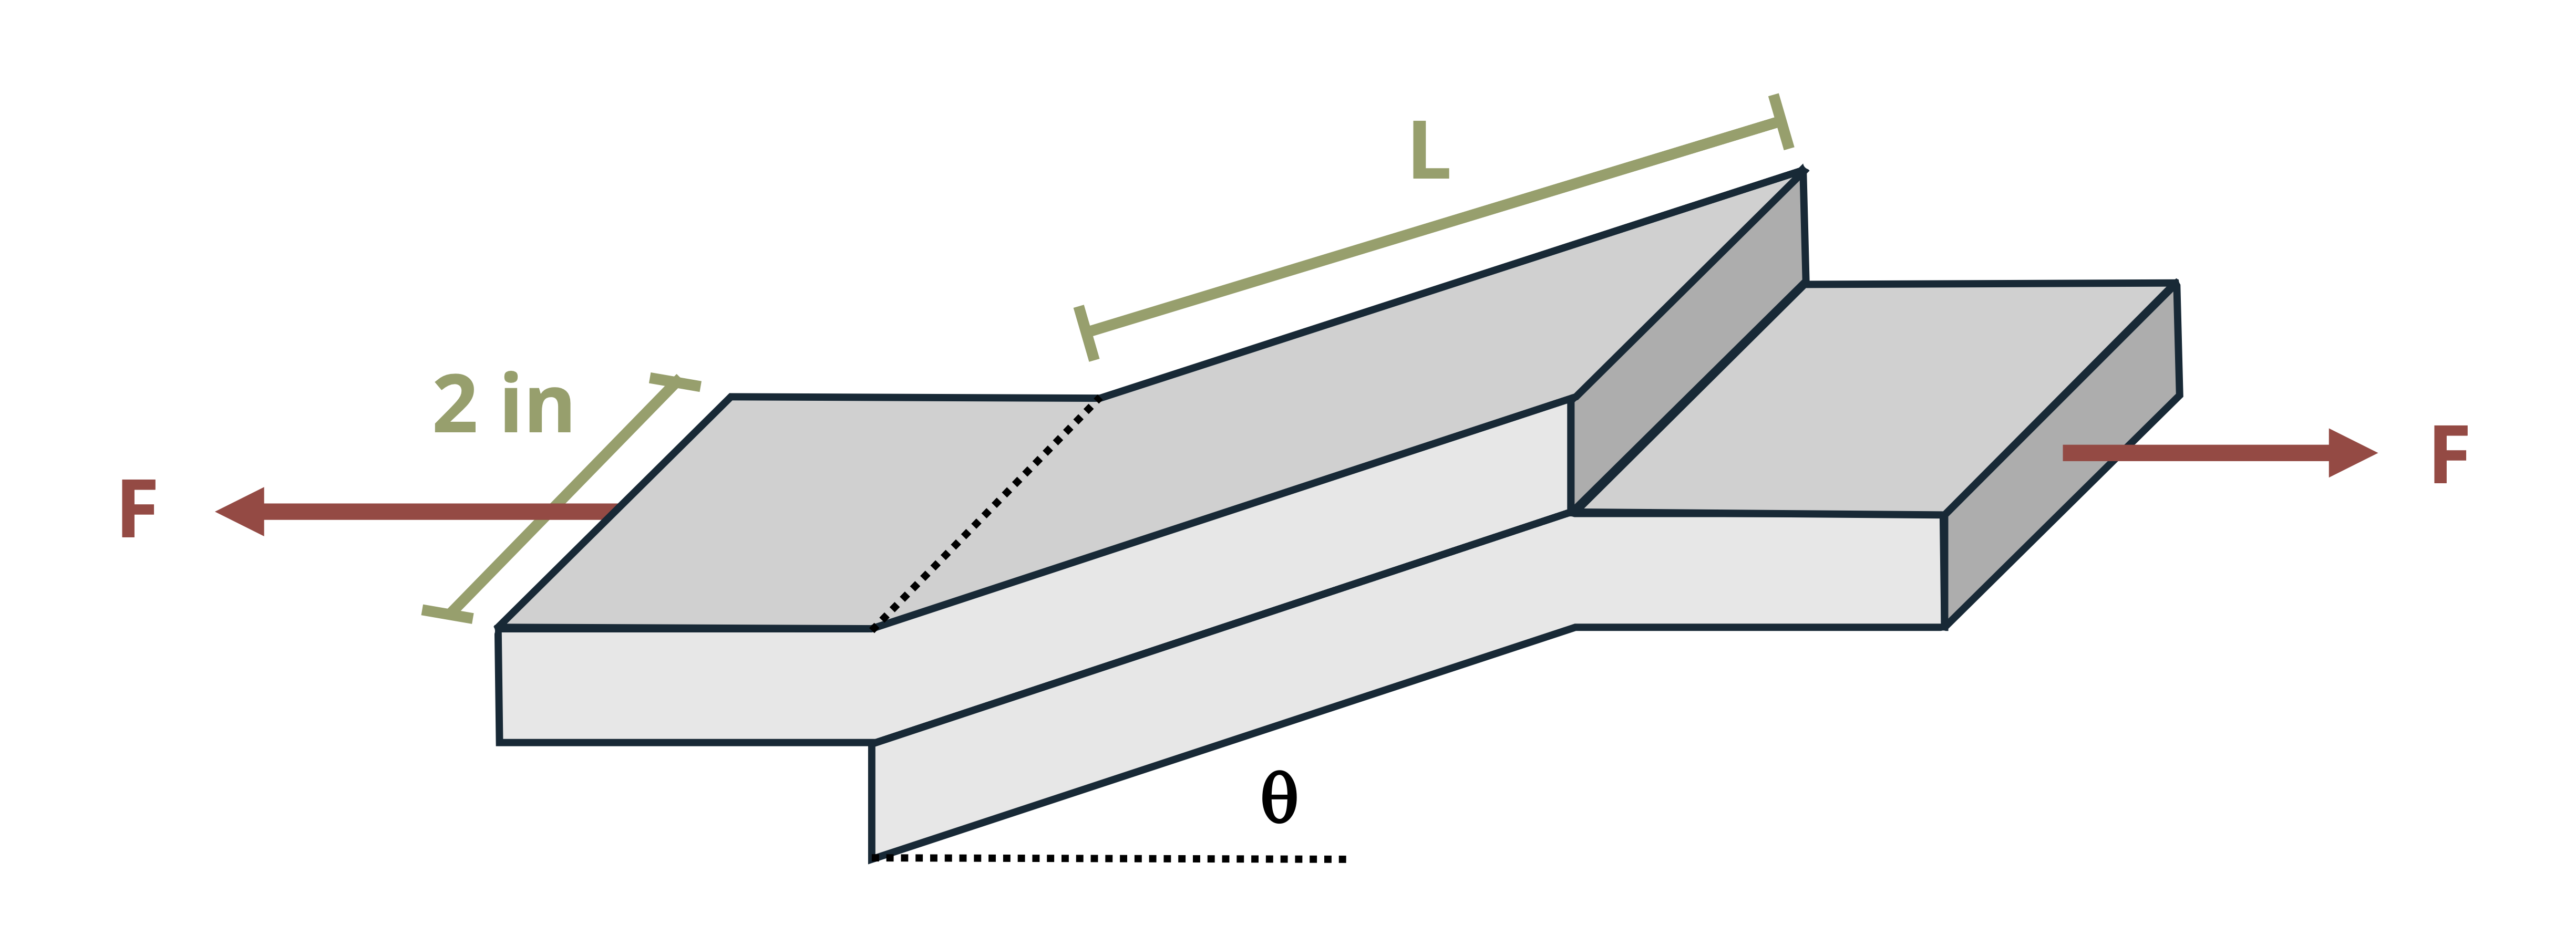
\includegraphics{images/153.png}

}

\caption{Figure 1: Two slanted brackets are glued together}

\end{figure}%

\begin{Shaded}
\begin{Highlighting}[]
\NormalTok{\#| standalone: true}
\NormalTok{\#| viewerHeight: 600}
\NormalTok{\#| components: [viewer]}

\NormalTok{from shiny import App, render, ui, reactive}
\NormalTok{import random}
\NormalTok{import asyncio}
\NormalTok{import io}
\NormalTok{import math}
\NormalTok{import string}
\NormalTok{from datetime import datetime}
\NormalTok{from pathlib import Path}

\NormalTok{def generate\_random\_letters(length):}
\NormalTok{    \# Generate a random string of letters of specified length}
\NormalTok{    return \textquotesingle{}\textquotesingle{}.join(random.choice(string.ascii\_lowercase) for \_ in range(length))  }

\NormalTok{problem\_ID="153"}
\NormalTok{F=reactive.Value("\_\_")}
\NormalTok{L=reactive.Value("\_\_")}
\NormalTok{Θ=reactive.Value("\_\_")}

\NormalTok{attempts=["Timestamp,Attempt,Answer,Feedback\textbackslash{}n"]}

\NormalTok{app\_ui = ui.page\_fluid(}
\NormalTok{    ui.markdown("**Please enter your ID number from your instructor and click to generate your problem**"),}
\NormalTok{    ui.input\_text("ID","", placeholder="Enter ID Number Here"),}
\NormalTok{    ui.input\_action\_button("generate\_problem", "Generate Problem", class\_="btn{-}primary"),}
\NormalTok{    ui.markdown("**Problem Statement**"),}
\NormalTok{    ui.output\_ui("ui\_problem\_statement"),}
\NormalTok{    ui.input\_text("answer","Your Answer in units of psi", placeholder="Please enter your answer"),}
\NormalTok{    ui.input\_action\_button("submit", "Submit Answer", class\_="btn{-}primary"),}
\NormalTok{    ui.download\_button("download", "Download File to Submit", class\_="btn{-}success"),}
\NormalTok{)}


\NormalTok{def server(input, output, session):}
\NormalTok{    \# Initialize a counter for attempts}
\NormalTok{    attempt\_counter = reactive.Value(0)}

\NormalTok{    @output}
\NormalTok{    @render.ui}
\NormalTok{    def ui\_problem\_statement():}
\NormalTok{        return[ui.markdown(f"Two slanted brackets are glued together as shown. If F = \{F()\} lb, L = \{L()\} in., and Θ = \{Θ()\} °, determine the shear stress parallel to the inclined plane. Assume loads are inline and there is no rotation.")]}
    
\NormalTok{    @reactive.Effect}
\NormalTok{    @reactive.event(input.generate\_problem)}
\NormalTok{    def randomize\_vars():}
\NormalTok{        random.seed(input.ID())}
\NormalTok{        F.set(random.randrange(200, 800, 10))}
\NormalTok{        L.set(random.randrange(20, 80, 1)/10)}
\NormalTok{        Θ.set(random.randrange(15, 30, 1))}
        

\NormalTok{    @reactive.Effect}
\NormalTok{    @reactive.event(input.submit)}
\NormalTok{    def \_():}
\NormalTok{        attempt\_counter.set(attempt\_counter() + 1)  \# Increment the attempt counter on each submission.}
    
\NormalTok{        instr= (F()*math.sin(math.radians(Θ()))/(L()*2))}
\NormalTok{        if math.isclose(float(input.answer()), instr, rel\_tol=0.001):}
\NormalTok{            check = "*Correct*"}
\NormalTok{            correct\_indicator = "JL"}
\NormalTok{        else:}
\NormalTok{            check = "*Not Correct.*"}
\NormalTok{            correct\_indicator = "JG"}

\NormalTok{        \# Generate random parts for the encoded attempt.}
\NormalTok{        random\_start = generate\_random\_letters(4)}
\NormalTok{        random\_middle = generate\_random\_letters(4)}
\NormalTok{        random\_end = generate\_random\_letters(4)}
\NormalTok{        encoded\_attempt = f"\{random\_start\}\{problem\_ID\}{-}\{random\_middle\}\{attempt\_counter()\}\{correct\_indicator\}{-}\{random\_end\}\{input.ID()\}"}

\NormalTok{        \# Store the most recent encoded attempt in a reactive value so it persists across submissions}
\NormalTok{        session.encoded\_attempt = reactive.Value(encoded\_attempt)}

\NormalTok{        \# Append the attempt data to the attempts list without the encoded attempt}
\NormalTok{        attempts.append(f"\{datetime.now()\}, \{attempt\_counter()\}, \{input.answer()\}, \{check\}\textbackslash{}n")}

\NormalTok{        \# Show feedback to the user.}
\NormalTok{        feedback = ui.markdown(f"Your answer of \{input.answer()\} is \{check\}. For reference in debugging this, the calculated instructor answer is \{instr\}")}
\NormalTok{        m = ui.modal(}
\NormalTok{            feedback,}
\NormalTok{            title="Feedback",}
\NormalTok{            easy\_close=True}
\NormalTok{        )}
\NormalTok{        ui.modal\_show(m)}

\NormalTok{    @session.download(filename=lambda: f"Problem\_Log{-}\{problem\_ID\}{-}\{input.ID()\}.csv")}
\NormalTok{    async def download():}
\NormalTok{        \# Start the CSV with the encoded attempt (without label)}
\NormalTok{        final\_encoded = session.encoded\_attempt() if session.encoded\_attempt is not None else "No attempts"}
\NormalTok{        yield f"\{final\_encoded\}\textbackslash{}n\textbackslash{}n"}
        
\NormalTok{        \# Write the header for the remaining CSV data once}
\NormalTok{        yield "Timestamp,Attempt,Answer,Feedback\textbackslash{}n"}
        
\NormalTok{        \# Write the attempts data, ensure that the header from the attempts list is not written again}
\NormalTok{        for attempt in attempts[1:]:  \# Skip the first element which is the header}
\NormalTok{            await asyncio.sleep(0.25)  \# This delay may not be necessary; adjust as needed}
\NormalTok{            yield attempt}


\NormalTok{\# App installation}
\NormalTok{app = App(app\_ui, server)}
\end{Highlighting}
\end{Shaded}

\chapter*{Problem 2.48}\label{problem-2.48}
\addcontentsline{toc}{chapter}{Problem 2.48}

\markboth{Problem 2.48}{Problem 2.48}

This is a dynamic rendering of the problem with dynamic variables based
on the username entered.

\section*{Problem Image}\label{problem-image-6}
\addcontentsline{toc}{section}{Problem Image}

\markright{Problem Image}

\begin{figure}[H]

{\centering 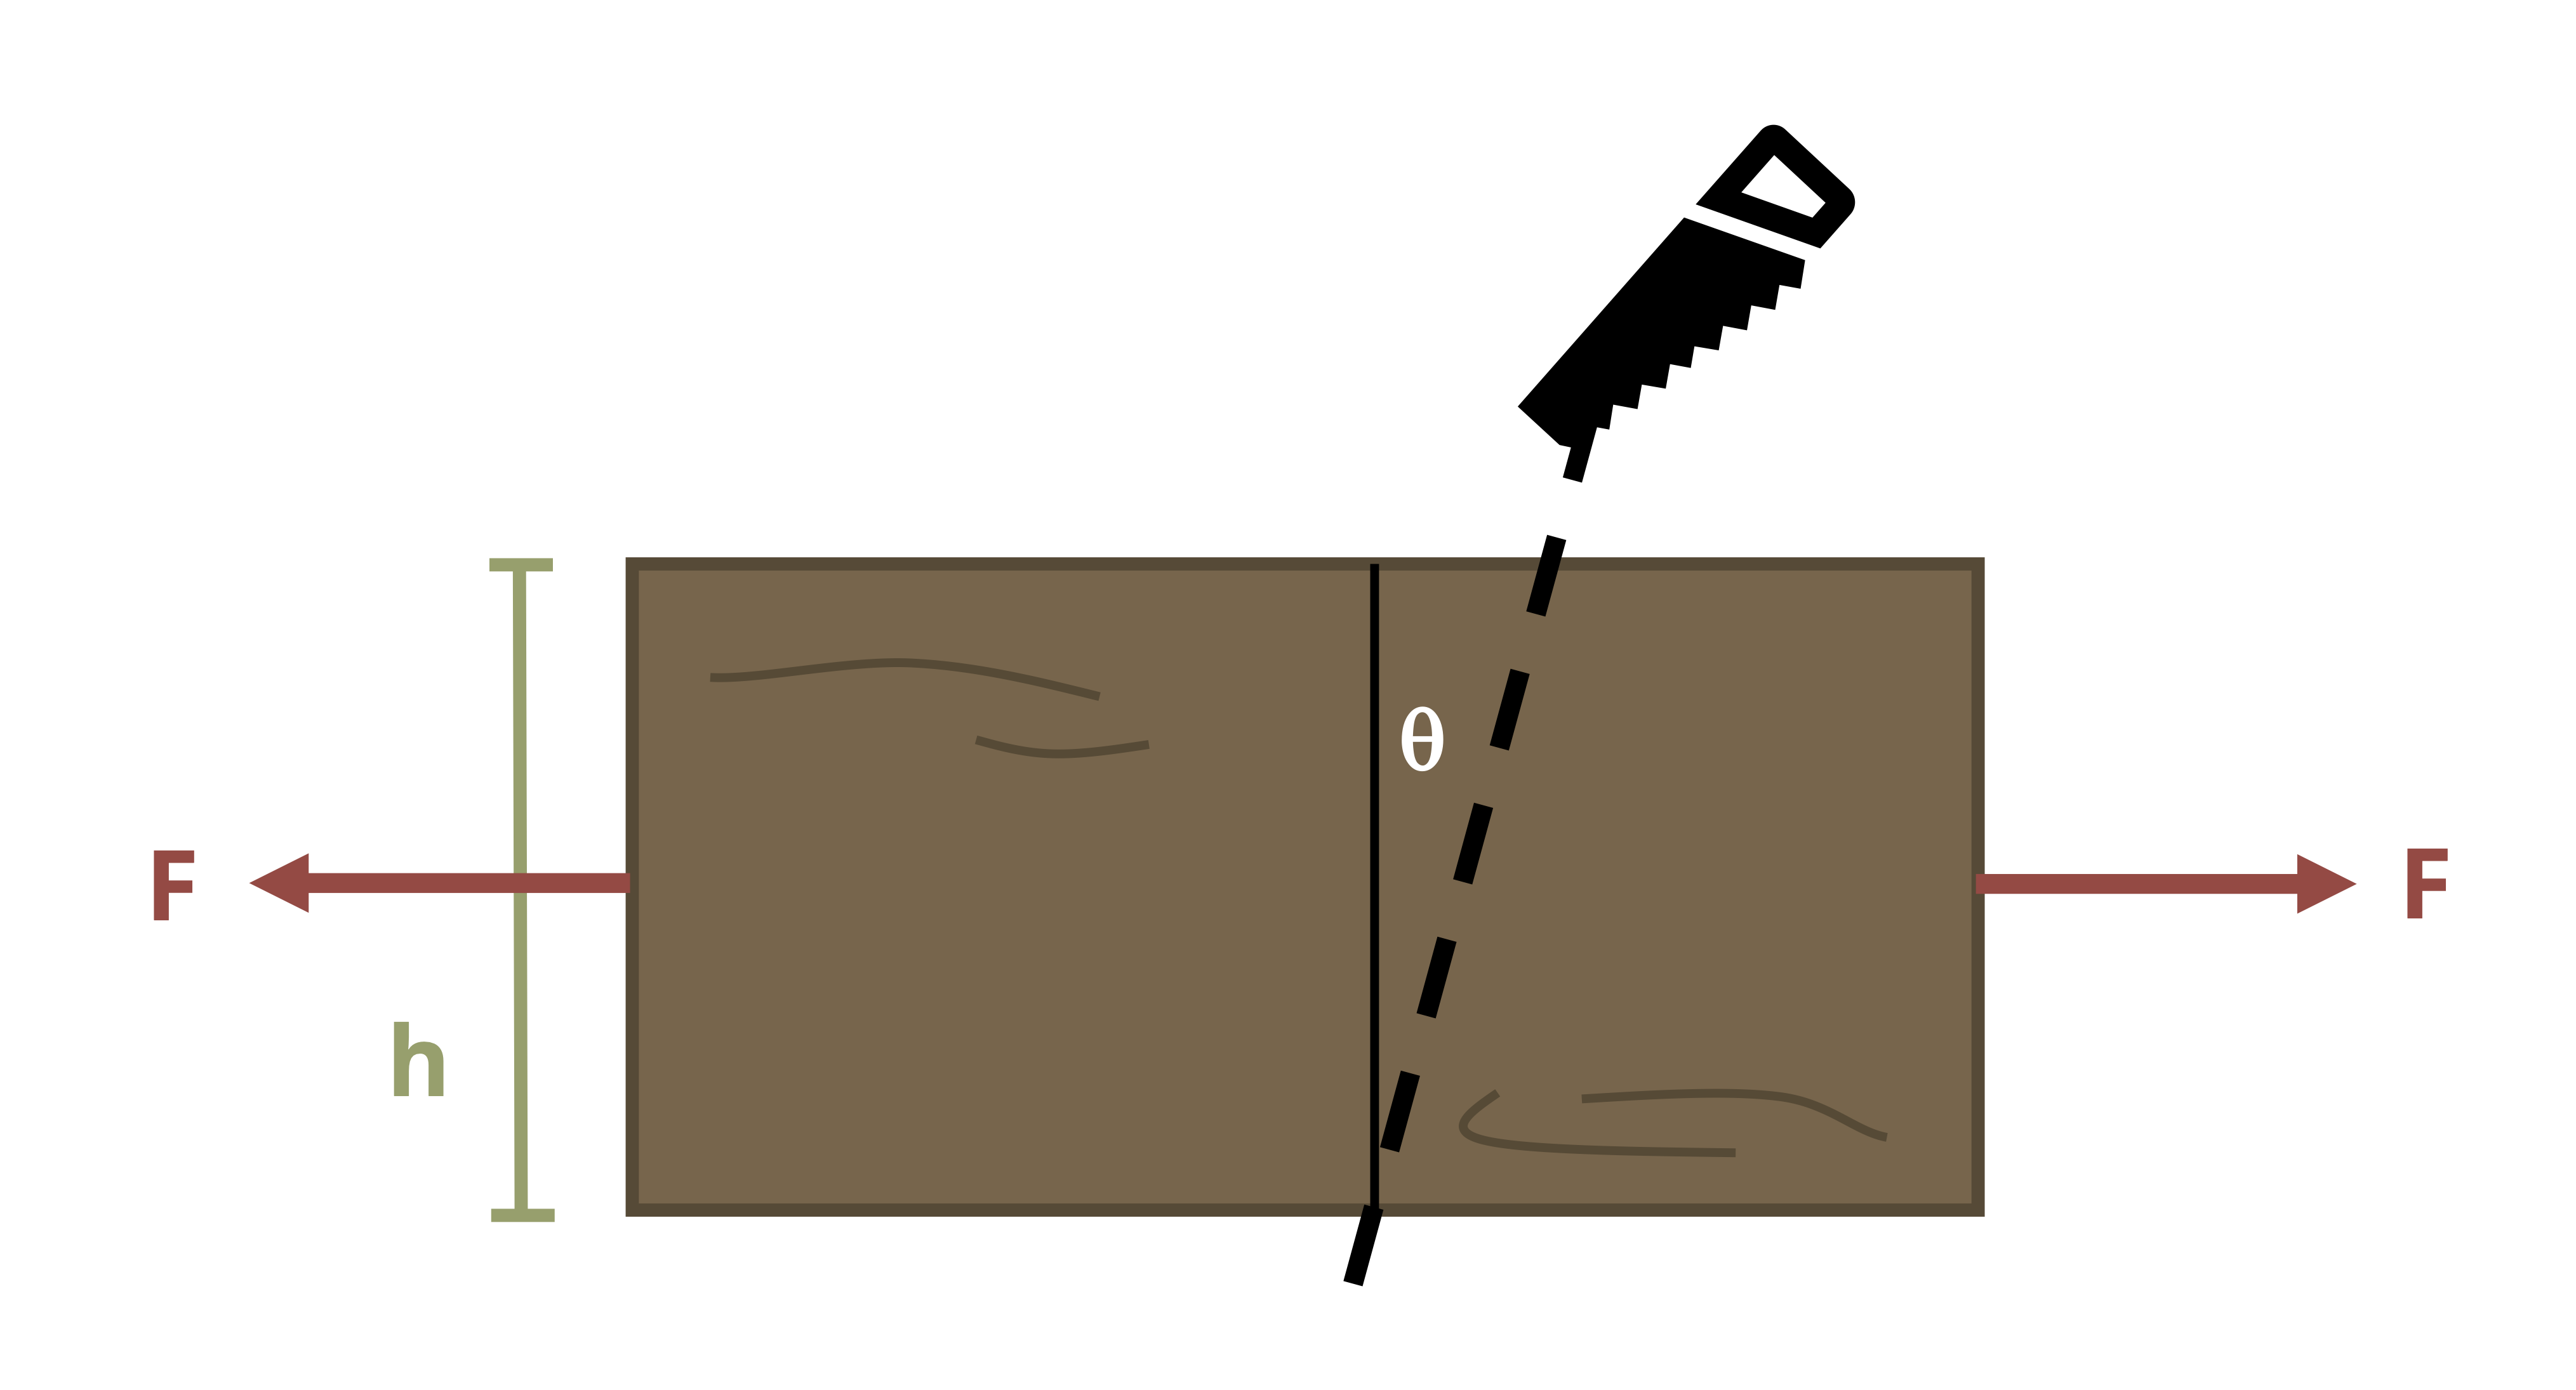
\includegraphics{images/156.png}

}

\caption{Figure 1: A 2 inch thick board is cut and then glued back
together along a line}

\end{figure}%

\begin{Shaded}
\begin{Highlighting}[]
\NormalTok{\#| standalone: true}
\NormalTok{\#| viewerHeight: 600}
\NormalTok{\#| components: [viewer]}

\NormalTok{from shiny import App, render, ui, reactive}
\NormalTok{import random}
\NormalTok{import asyncio}
\NormalTok{import io}
\NormalTok{import math}
\NormalTok{import string}
\NormalTok{from datetime import datetime}
\NormalTok{from pathlib import Path}

\NormalTok{def generate\_random\_letters(length):}
\NormalTok{    \# Generate a random string of letters of specified length}
\NormalTok{    return \textquotesingle{}\textquotesingle{}.join(random.choice(string.ascii\_lowercase) for \_ in range(length))  }

\NormalTok{problem\_ID="156"}
\NormalTok{F=reactive.Value("\_\_")}
\NormalTok{h=reactive.Value("\_\_")}
\NormalTok{Θ=reactive.Value("\_\_")}

\NormalTok{attempts=["Timestamp,Attempt,Answer,Feedback\textbackslash{}n"]}

\NormalTok{app\_ui = ui.page\_fluid(}
\NormalTok{    ui.markdown("**Please enter your ID number from your instructor and click to generate your problem**"),}
\NormalTok{    ui.input\_text("ID","", placeholder="Enter ID Number Here"),}
\NormalTok{    ui.input\_action\_button("generate\_problem", "Generate Problem", class\_="btn{-}primary"),}
\NormalTok{    ui.markdown("**Problem Statement**"),}
\NormalTok{    ui.output\_ui("ui\_problem\_statement"),}
\NormalTok{    ui.input\_text("answer","Your Answer in units of psi", placeholder="Please enter your answer"),}
\NormalTok{    ui.input\_action\_button("submit", "Submit Answer", class\_="btn{-}primary"),}
\NormalTok{    ui.download\_button("download", "Download File to Submit", class\_="btn{-}success"),}
\NormalTok{)}


\NormalTok{def server(input, output, session):}
\NormalTok{    \# Initialize a counter for attempts}
\NormalTok{    attempt\_counter = reactive.Value(0)}

\NormalTok{    @output}
\NormalTok{    @render.ui}
\NormalTok{    def ui\_problem\_statement():}
\NormalTok{        return[ui.markdown(f"A 2 inch thick board is cut and then glued back together along a line that is Θ = \{Θ()\} ° off the vertical as shown. If height h = \{h()\} in. and F = \{F()\} lb, determine the normal stress along the cut line.")]}
    
\NormalTok{    @reactive.Effect}
\NormalTok{    @reactive.event(input.generate\_problem)}
\NormalTok{    def randomize\_vars():}
\NormalTok{        random.seed(input.ID())}
\NormalTok{        F.set(random.randrange(2000, 6000, 100))}
\NormalTok{        h.set(random.randrange(50, 150, 1)/10)}
\NormalTok{        Θ.set(random.randrange(10, 20, 1))}
        

\NormalTok{    @reactive.Effect}
\NormalTok{    @reactive.event(input.submit)}
\NormalTok{    def \_():}
\NormalTok{        attempt\_counter.set(attempt\_counter() + 1)  \# Increment the attempt counter on each submission.}
        
\NormalTok{        instr= (F()/(2*h()))*(math.cos(math.radians(Θ()))**2)}
\NormalTok{        if math.isclose(float(input.answer()), instr, rel\_tol=0.001):}
\NormalTok{            check = "*Correct*"}
\NormalTok{            correct\_indicator = "JL"}
\NormalTok{        else:}
\NormalTok{            check = "*Not Correct.*"}
\NormalTok{            correct\_indicator = "JG"}

\NormalTok{        \# Generate random parts for the encoded attempt.}
\NormalTok{        random\_start = generate\_random\_letters(4)}
\NormalTok{        random\_middle = generate\_random\_letters(4)}
\NormalTok{        random\_end = generate\_random\_letters(4)}
\NormalTok{        encoded\_attempt = f"\{random\_start\}\{problem\_ID\}{-}\{random\_middle\}\{attempt\_counter()\}\{correct\_indicator\}{-}\{random\_end\}\{input.ID()\}"}

\NormalTok{        \# Store the most recent encoded attempt in a reactive value so it persists across submissions}
\NormalTok{        session.encoded\_attempt = reactive.Value(encoded\_attempt)}

\NormalTok{        \# Append the attempt data to the attempts list without the encoded attempt}
\NormalTok{        attempts.append(f"\{datetime.now()\}, \{attempt\_counter()\}, \{input.answer()\}, \{check\}\textbackslash{}n")}

\NormalTok{        \# Show feedback to the user.}
\NormalTok{        feedback = ui.markdown(f"Your answer of \{input.answer()\} is \{check\}. For reference in debugging this, the calculated instructor answer is \{instr\}")}
\NormalTok{        m = ui.modal(}
\NormalTok{            feedback,}
\NormalTok{            title="Feedback",}
\NormalTok{            easy\_close=True}
\NormalTok{        )}
\NormalTok{        ui.modal\_show(m)}

\NormalTok{    @session.download(filename=lambda: f"Problem\_Log{-}\{problem\_ID\}{-}\{input.ID()\}.csv")}
\NormalTok{    async def download():}
\NormalTok{        \# Start the CSV with the encoded attempt (without label)}
\NormalTok{        final\_encoded = session.encoded\_attempt() if session.encoded\_attempt is not None else "No attempts"}
\NormalTok{        yield f"\{final\_encoded\}\textbackslash{}n\textbackslash{}n"}
        
\NormalTok{        \# Write the header for the remaining CSV data once}
\NormalTok{        yield "Timestamp,Attempt,Answer,Feedback\textbackslash{}n"}
        
\NormalTok{        \# Write the attempts data, ensure that the header from the attempts list is not written again}
\NormalTok{        for attempt in attempts[1:]:  \# Skip the first element which is the header}
\NormalTok{            await asyncio.sleep(0.25)  \# This delay may not be necessary; adjust as needed}
\NormalTok{            yield attempt}


\NormalTok{\# App installation}
\NormalTok{app = App(app\_ui, server)}
\end{Highlighting}
\end{Shaded}

\chapter*{Problem 4.37}\label{problem-4.37}
\addcontentsline{toc}{chapter}{Problem 4.37}

\markboth{Problem 4.37}{Problem 4.37}

This is a dynamic rendering of the problem with dynamic variables based
on the username entered.

\section*{Problem Image}\label{problem-image-7}
\addcontentsline{toc}{section}{Problem Image}

\markright{Problem Image}

\begin{figure}[H]

{\centering 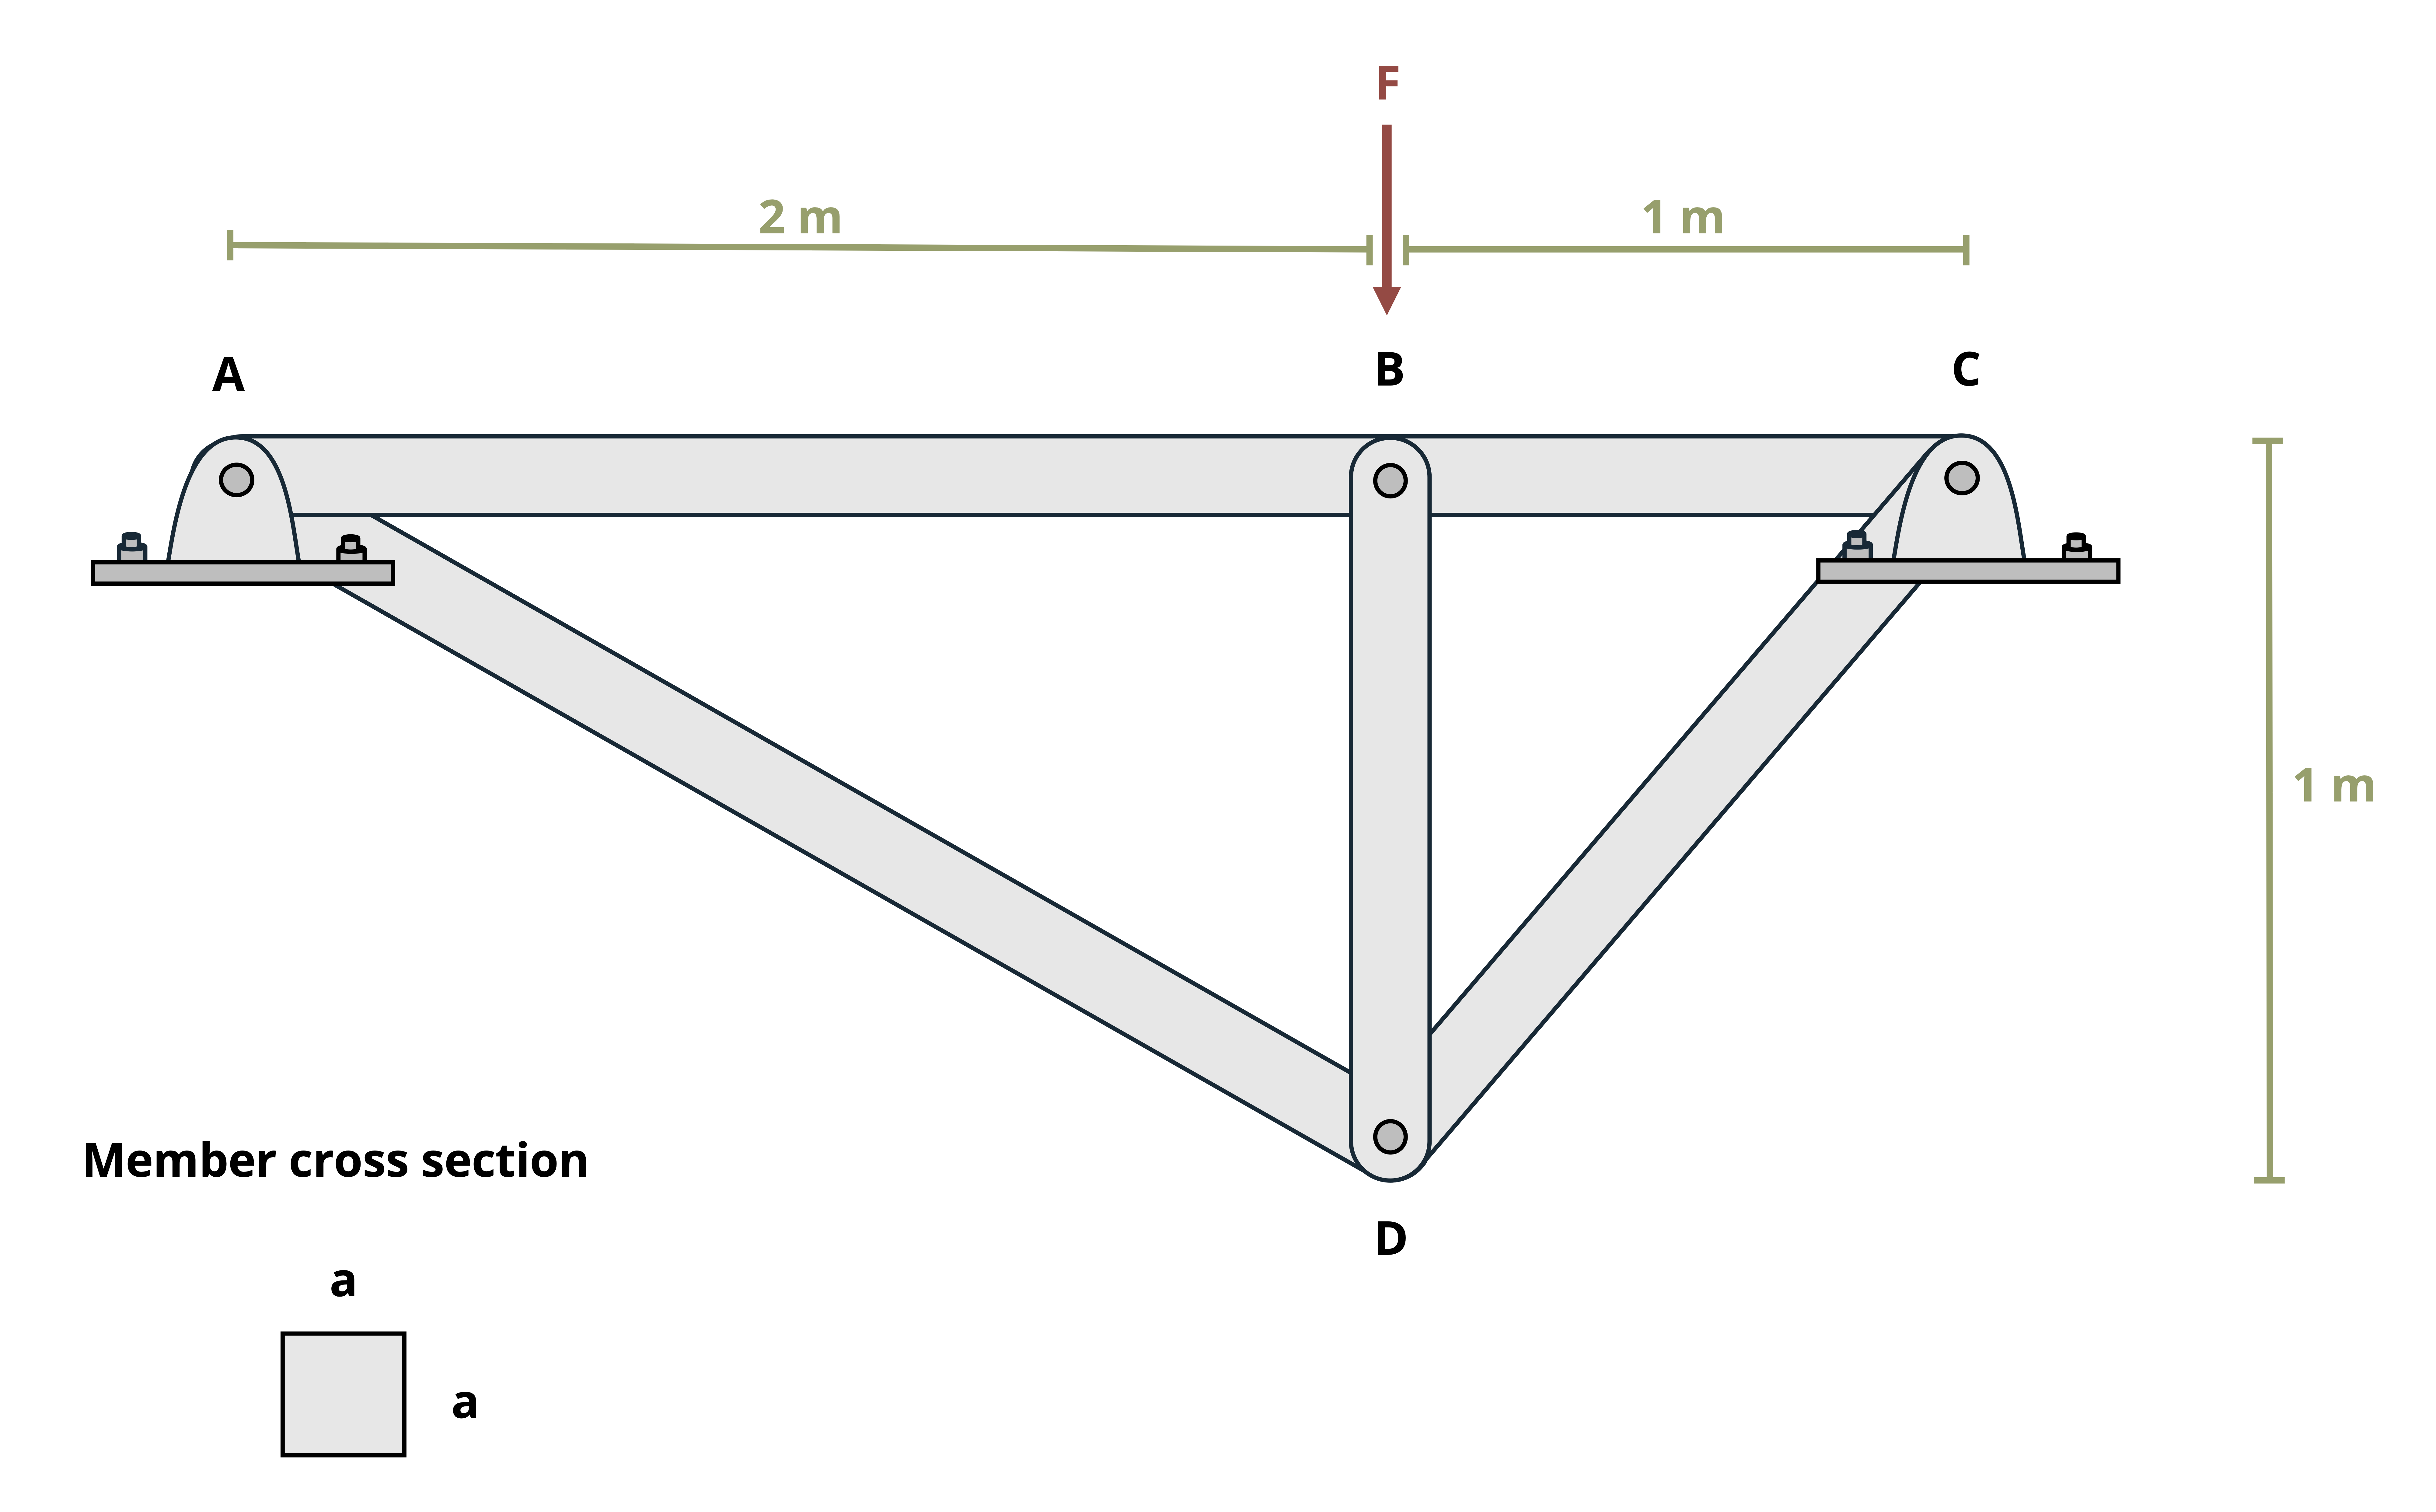
\includegraphics{images/157.png}

}

\caption{Figure 1: A small truss is constructed with solid square wood
members}

\end{figure}%

\begin{Shaded}
\begin{Highlighting}[]
\NormalTok{\#| standalone: true}
\NormalTok{\#| viewerHeight: 600}
\NormalTok{\#| components: [viewer]}

\NormalTok{from shiny import App, render, ui, reactive}
\NormalTok{import random}
\NormalTok{import asyncio}
\NormalTok{import io}
\NormalTok{import math}
\NormalTok{import string}
\NormalTok{from datetime import datetime}
\NormalTok{from pathlib import Path}

\NormalTok{def generate\_random\_letters(length):}
\NormalTok{    \# Generate a random string of letters of specified length}
\NormalTok{    return \textquotesingle{}\textquotesingle{}.join(random.choice(string.ascii\_lowercase) for \_ in range(length))  }

\NormalTok{problem\_ID="157"}
\NormalTok{F=reactive.Value("\_\_")}
\NormalTok{FS=reactive.Value("\_\_")}
\NormalTok{σfail=reactive.Value("\_\_")}

\NormalTok{attempts=["Timestamp,Attempt,Answer,Feedback\textbackslash{}n"]}

\NormalTok{app\_ui = ui.page\_fluid(}
\NormalTok{    ui.markdown("**Please enter your ID number from your instructor and click to generate your problem**"),}
\NormalTok{    ui.input\_text("ID","", placeholder="Enter ID Number Here"),}
\NormalTok{    ui.input\_action\_button("generate\_problem", "Generate Problem", class\_="btn{-}primary"),}
\NormalTok{    ui.markdown("**Problem Statement**"),}
\NormalTok{    ui.output\_ui("ui\_problem\_statement"),}
\NormalTok{    ui.input\_text("answer","Your Answer in units of centimeters", placeholder="Please enter your answer"),}
\NormalTok{    ui.input\_action\_button("submit", "Submit Answer", class\_="btn{-}primary"),}
\NormalTok{    ui.download\_button("download", "Download File to Submit", class\_="btn{-}success"),}
\NormalTok{)}


\NormalTok{def server(input, output, session):}
\NormalTok{    \# Initialize a counter for attempts}
\NormalTok{    attempt\_counter = reactive.Value(0)}

\NormalTok{    @output}
\NormalTok{    @render.ui}
\NormalTok{    def ui\_problem\_statement():}
\NormalTok{        return[ui.markdown(f"A small truss is constructed with solid square wood members and subjected to a load of F = \{F()\} kN. Determine the minimum dimension, a, of the member so that the truss will have a factor of safety of \{FS()\}. All members have the same cross{-}section. The wood has a failure stress of σ\textless{}sub\textgreater{}fail\textless{}/sub\textgreater{} = \{σfail()\} MPa.")]}
    
\NormalTok{    @reactive.Effect}
\NormalTok{    @reactive.event(input.generate\_problem)}
\NormalTok{    def randomize\_vars():}
\NormalTok{        random.seed(input.ID())}
\NormalTok{        F.set(random.randrange(15, 50, 1))}
\NormalTok{        FS.set(random.randrange(15, 40, 1)/10)}
\NormalTok{        σfail.set(random.randrange(40, 60, 1))}
        

\NormalTok{    @reactive.Effect}
\NormalTok{    @reactive.event(input.submit)}
\NormalTok{    def \_():}
\NormalTok{        attempt\_counter.set(attempt\_counter() + 1)  \# Increment the attempt counter on each submission.}
    
\NormalTok{        dl = FS()*F()}
\NormalTok{        A = (dl/(σfail()*10**3))*100*100}
\NormalTok{        instr= math.sqrt(A)}
\NormalTok{        if math.isclose(float(input.answer()), instr, rel\_tol=0.001):}
\NormalTok{            check = "*Correct*"}
\NormalTok{            correct\_indicator = "JL"}
\NormalTok{        else:}
\NormalTok{            check = "*Not Correct.*"}
\NormalTok{            correct\_indicator = "JG"}

\NormalTok{        \# Generate random parts for the encoded attempt.}
\NormalTok{        random\_start = generate\_random\_letters(4)}
\NormalTok{        random\_middle = generate\_random\_letters(4)}
\NormalTok{        random\_end = generate\_random\_letters(4)}
\NormalTok{        encoded\_attempt = f"\{random\_start\}\{problem\_ID\}{-}\{random\_middle\}\{attempt\_counter()\}\{correct\_indicator\}{-}\{random\_end\}\{input.ID()\}"}

\NormalTok{        \# Store the most recent encoded attempt in a reactive value so it persists across submissions}
\NormalTok{        session.encoded\_attempt = reactive.Value(encoded\_attempt)}

\NormalTok{        \# Append the attempt data to the attempts list without the encoded attempt}
\NormalTok{        attempts.append(f"\{datetime.now()\}, \{attempt\_counter()\}, \{input.answer()\}, \{check\}\textbackslash{}n")}

\NormalTok{        \# Show feedback to the user.}
\NormalTok{        feedback = ui.markdown(f"Your answer of \{input.answer()\} is \{check\}. For reference in debugging this, the calculated instructor answer is \{instr\}")}
\NormalTok{        m = ui.modal(}
\NormalTok{            feedback,}
\NormalTok{            title="Feedback",}
\NormalTok{            easy\_close=True}
\NormalTok{        )}
\NormalTok{        ui.modal\_show(m)}

\NormalTok{    @session.download(filename=lambda: f"Problem\_Log{-}\{problem\_ID\}{-}\{input.ID()\}.csv")}
\NormalTok{    async def download():}
\NormalTok{        \# Start the CSV with the encoded attempt (without label)}
\NormalTok{        final\_encoded = session.encoded\_attempt() if session.encoded\_attempt is not None else "No attempts"}
\NormalTok{        yield f"\{final\_encoded\}\textbackslash{}n\textbackslash{}n"}
        
\NormalTok{        \# Write the header for the remaining CSV data once}
\NormalTok{        yield "Timestamp,Attempt,Answer,Feedback\textbackslash{}n"}
        
\NormalTok{        \# Write the attempts data, ensure that the header from the attempts list is not written again}
\NormalTok{        for attempt in attempts[1:]:  \# Skip the first element which is the header}
\NormalTok{            await asyncio.sleep(0.25)  \# This delay may not be necessary; adjust as needed}
\NormalTok{            yield attempt}


\NormalTok{\# App installation}
\NormalTok{app = App(app\_ui, server)}
\end{Highlighting}
\end{Shaded}

\chapter*{Problem 2.21}\label{problem-2.21}
\addcontentsline{toc}{chapter}{Problem 2.21}

\markboth{Problem 2.21}{Problem 2.21}

This is a dynamic rendering of the problem with dynamic variables based
on the username entered.

\section*{Problem Image}\label{problem-image-8}
\addcontentsline{toc}{section}{Problem Image}

\markright{Problem Image}

\begin{figure}[H]

{\centering 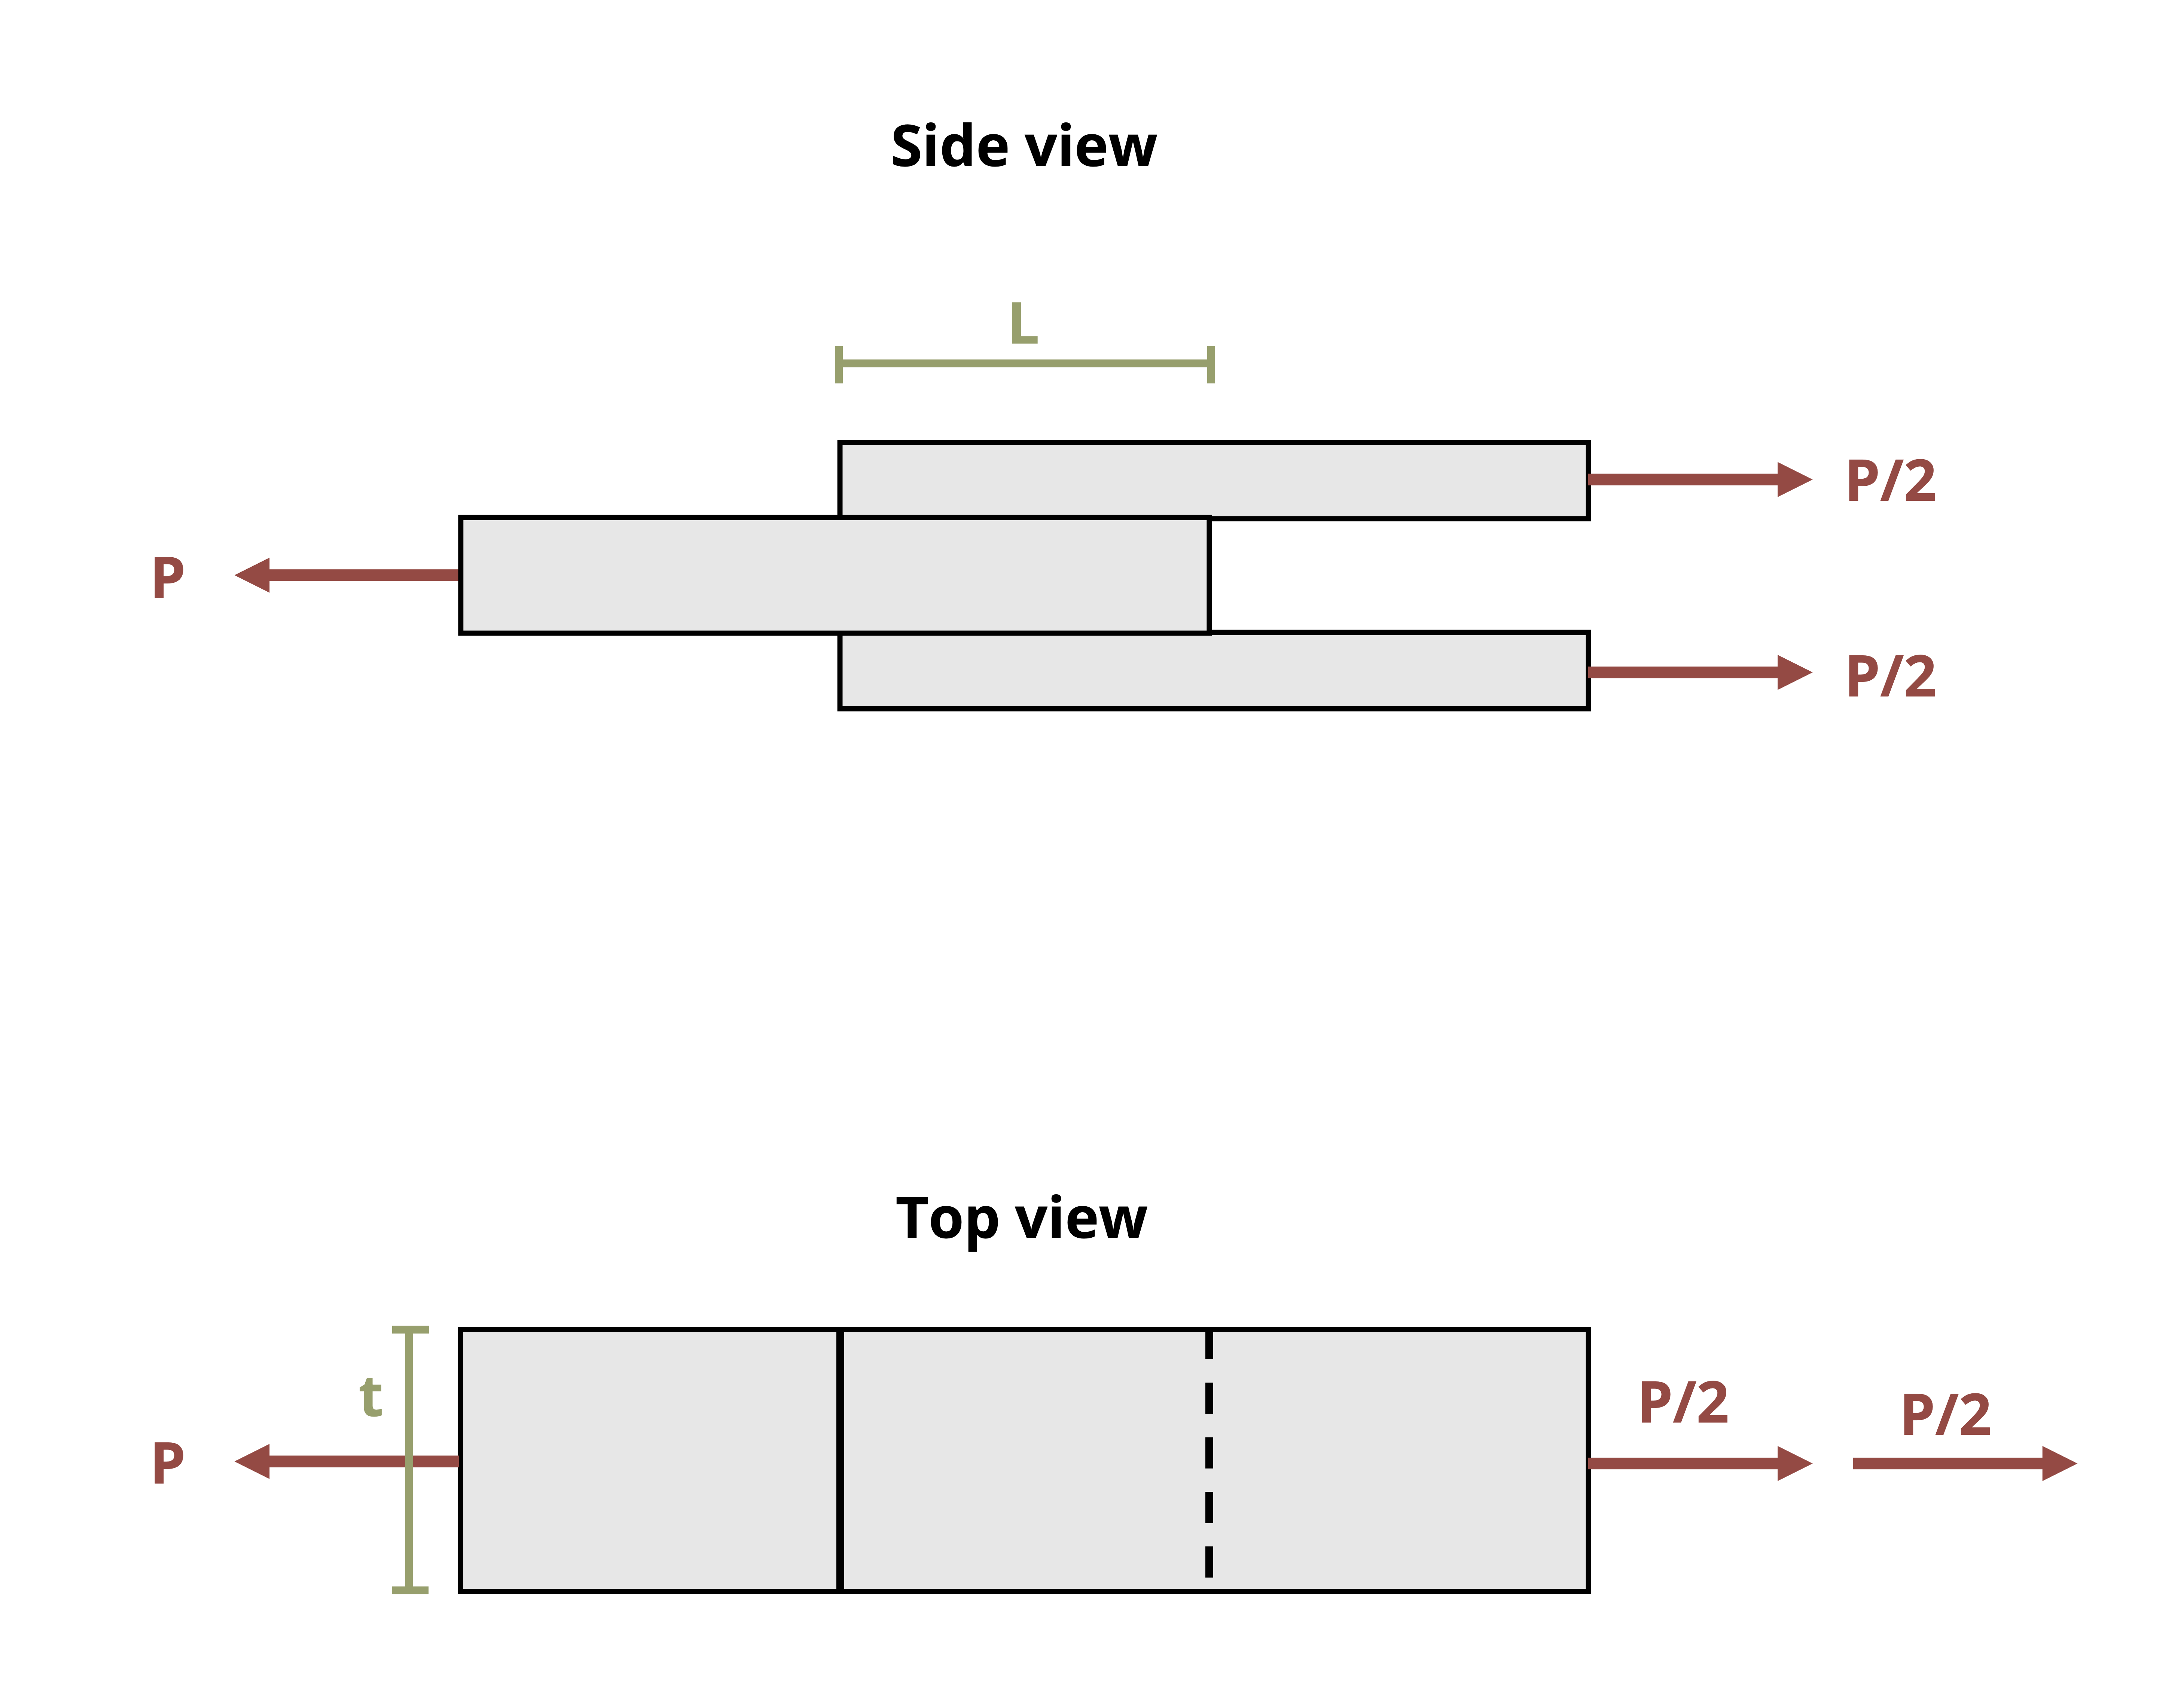
\includegraphics{images/164.png}

}

\caption{Figure 1: A double lap joint is glued together}

\end{figure}%

\begin{Shaded}
\begin{Highlighting}[]
\NormalTok{\#| standalone: true}
\NormalTok{\#| viewerHeight: 600}
\NormalTok{\#| components: [viewer]}

\NormalTok{from shiny import App, render, ui, reactive}
\NormalTok{import random}
\NormalTok{import asyncio}
\NormalTok{import io}
\NormalTok{import math}
\NormalTok{import string}
\NormalTok{from datetime import datetime}
\NormalTok{from pathlib import Path}

\NormalTok{def generate\_random\_letters(length):}
\NormalTok{    \# Generate a random string of letters of specified length}
\NormalTok{    return \textquotesingle{}\textquotesingle{}.join(random.choice(string.ascii\_lowercase) for \_ in range(length))  }

\NormalTok{problem\_ID="164"}
\NormalTok{τfail=reactive.Value("\_\_")}
\NormalTok{L=reactive.Value("\_\_")}
\NormalTok{t=reactive.Value("\_\_")}

\NormalTok{attempts=["Timestamp,Attempt,Answer,Feedback\textbackslash{}n"]}

\NormalTok{app\_ui = ui.page\_fluid(}
\NormalTok{    ui.markdown("**Please enter your ID number from your instructor and click to generate your problem**"),}
\NormalTok{    ui.input\_text("ID","", placeholder="Enter ID Number Here"),}
\NormalTok{    ui.input\_action\_button("generate\_problem", "Generate Problem", class\_="btn{-}primary"),}
\NormalTok{    ui.markdown("**Problem Statement**"),}
\NormalTok{    ui.output\_ui("ui\_problem\_statement"),}
\NormalTok{    ui.input\_text("answer","Your Answer in units of kips", placeholder="Please enter your answer"),}
\NormalTok{    ui.input\_action\_button("submit", "Submit Answer", class\_="btn{-}primary"),}
\NormalTok{    ui.download\_button("download", "Download File to Submit", class\_="btn{-}success"),}
\NormalTok{)}


\NormalTok{def server(input, output, session):}
\NormalTok{    \# Initialize a counter for attempts}
\NormalTok{    attempt\_counter = reactive.Value(0)}

\NormalTok{    @output}
\NormalTok{    @render.ui}
\NormalTok{    def ui\_problem\_statement():}
\NormalTok{        return[ui.markdown(f"A double lap joint is glued together using glue with a shear stress failure strength of \{τfail()\} psi. If dimensions L = \{L()\} in. and t = \{t()\} in., what is the maximum load P that the joint can withstand? Assume the load is evenly distributed across the joint on both sides.")]}
    
\NormalTok{    @reactive.Effect}
\NormalTok{    @reactive.event(input.generate\_problem)}
\NormalTok{    def randomize\_vars():}
\NormalTok{        random.seed(input.ID())}
\NormalTok{        τfail.set(random.randrange(7000, 9000, 100))}
\NormalTok{        L.set(random.randrange(40, 100, 1)/10)}
\NormalTok{        t.set(random.randrange(40, 100, 1)/10)}
        

\NormalTok{    @reactive.Effect}
\NormalTok{    @reactive.event(input.submit)}
\NormalTok{    def \_():}
\NormalTok{        attempt\_counter.set(attempt\_counter() + 1)  \# Increment the attempt counter on each submission.}
    
\NormalTok{        A = L()*t()*2}
\NormalTok{        instr= (τfail()*A)/1000}
\NormalTok{        if math.isclose(float(input.answer()), instr, rel\_tol=0.001):}
\NormalTok{            check = "*Correct*"}
\NormalTok{            correct\_indicator = "JL"}
\NormalTok{        else:}
\NormalTok{            check = "*Not Correct.*"}
\NormalTok{            correct\_indicator = "JG"}

\NormalTok{        \# Generate random parts for the encoded attempt.}
\NormalTok{        random\_start = generate\_random\_letters(4)}
\NormalTok{        random\_middle = generate\_random\_letters(4)}
\NormalTok{        random\_end = generate\_random\_letters(4)}
\NormalTok{        encoded\_attempt = f"\{random\_start\}\{problem\_ID\}{-}\{random\_middle\}\{attempt\_counter()\}\{correct\_indicator\}{-}\{random\_end\}\{input.ID()\}"}

\NormalTok{        \# Store the most recent encoded attempt in a reactive value so it persists across submissions}
\NormalTok{        session.encoded\_attempt = reactive.Value(encoded\_attempt)}

\NormalTok{        \# Append the attempt data to the attempts list without the encoded attempt}
\NormalTok{        attempts.append(f"\{datetime.now()\}, \{attempt\_counter()\}, \{input.answer()\}, \{check\}\textbackslash{}n")}

\NormalTok{        \# Show feedback to the user.}
\NormalTok{        feedback = ui.markdown(f"Your answer of \{input.answer()\} is \{check\}. For reference in debugging this, the calculated instructor answer is \{instr\}")}
\NormalTok{        m = ui.modal(}
\NormalTok{            feedback,}
\NormalTok{            title="Feedback",}
\NormalTok{            easy\_close=True}
\NormalTok{        )}
\NormalTok{        ui.modal\_show(m)}

\NormalTok{    @session.download(filename=lambda: f"Problem\_Log{-}\{problem\_ID\}{-}\{input.ID()\}.csv")}
\NormalTok{    async def download():}
\NormalTok{        \# Start the CSV with the encoded attempt (without label)}
\NormalTok{        final\_encoded = session.encoded\_attempt() if session.encoded\_attempt is not None else "No attempts"}
\NormalTok{        yield f"\{final\_encoded\}\textbackslash{}n\textbackslash{}n"}
        
\NormalTok{        \# Write the header for the remaining CSV data once}
\NormalTok{        yield "Timestamp,Attempt,Answer,Feedback\textbackslash{}n"}
        
\NormalTok{        \# Write the attempts data, ensure that the header from the attempts list is not written again}
\NormalTok{        for attempt in attempts[1:]:  \# Skip the first element which is the header}
\NormalTok{            await asyncio.sleep(0.25)  \# This delay may not be necessary; adjust as needed}
\NormalTok{            yield attempt}


\NormalTok{\# App installation}
\NormalTok{app = App(app\_ui, server)}
\end{Highlighting}
\end{Shaded}

\chapter*{Problem 2.22}\label{problem-2.22}
\addcontentsline{toc}{chapter}{Problem 2.22}

\markboth{Problem 2.22}{Problem 2.22}

This is a dynamic rendering of the problem with dynamic variables based
on the username entered.

\section{Problem Image}\label{problem-image-9}

\begin{figure}[H]

{\centering 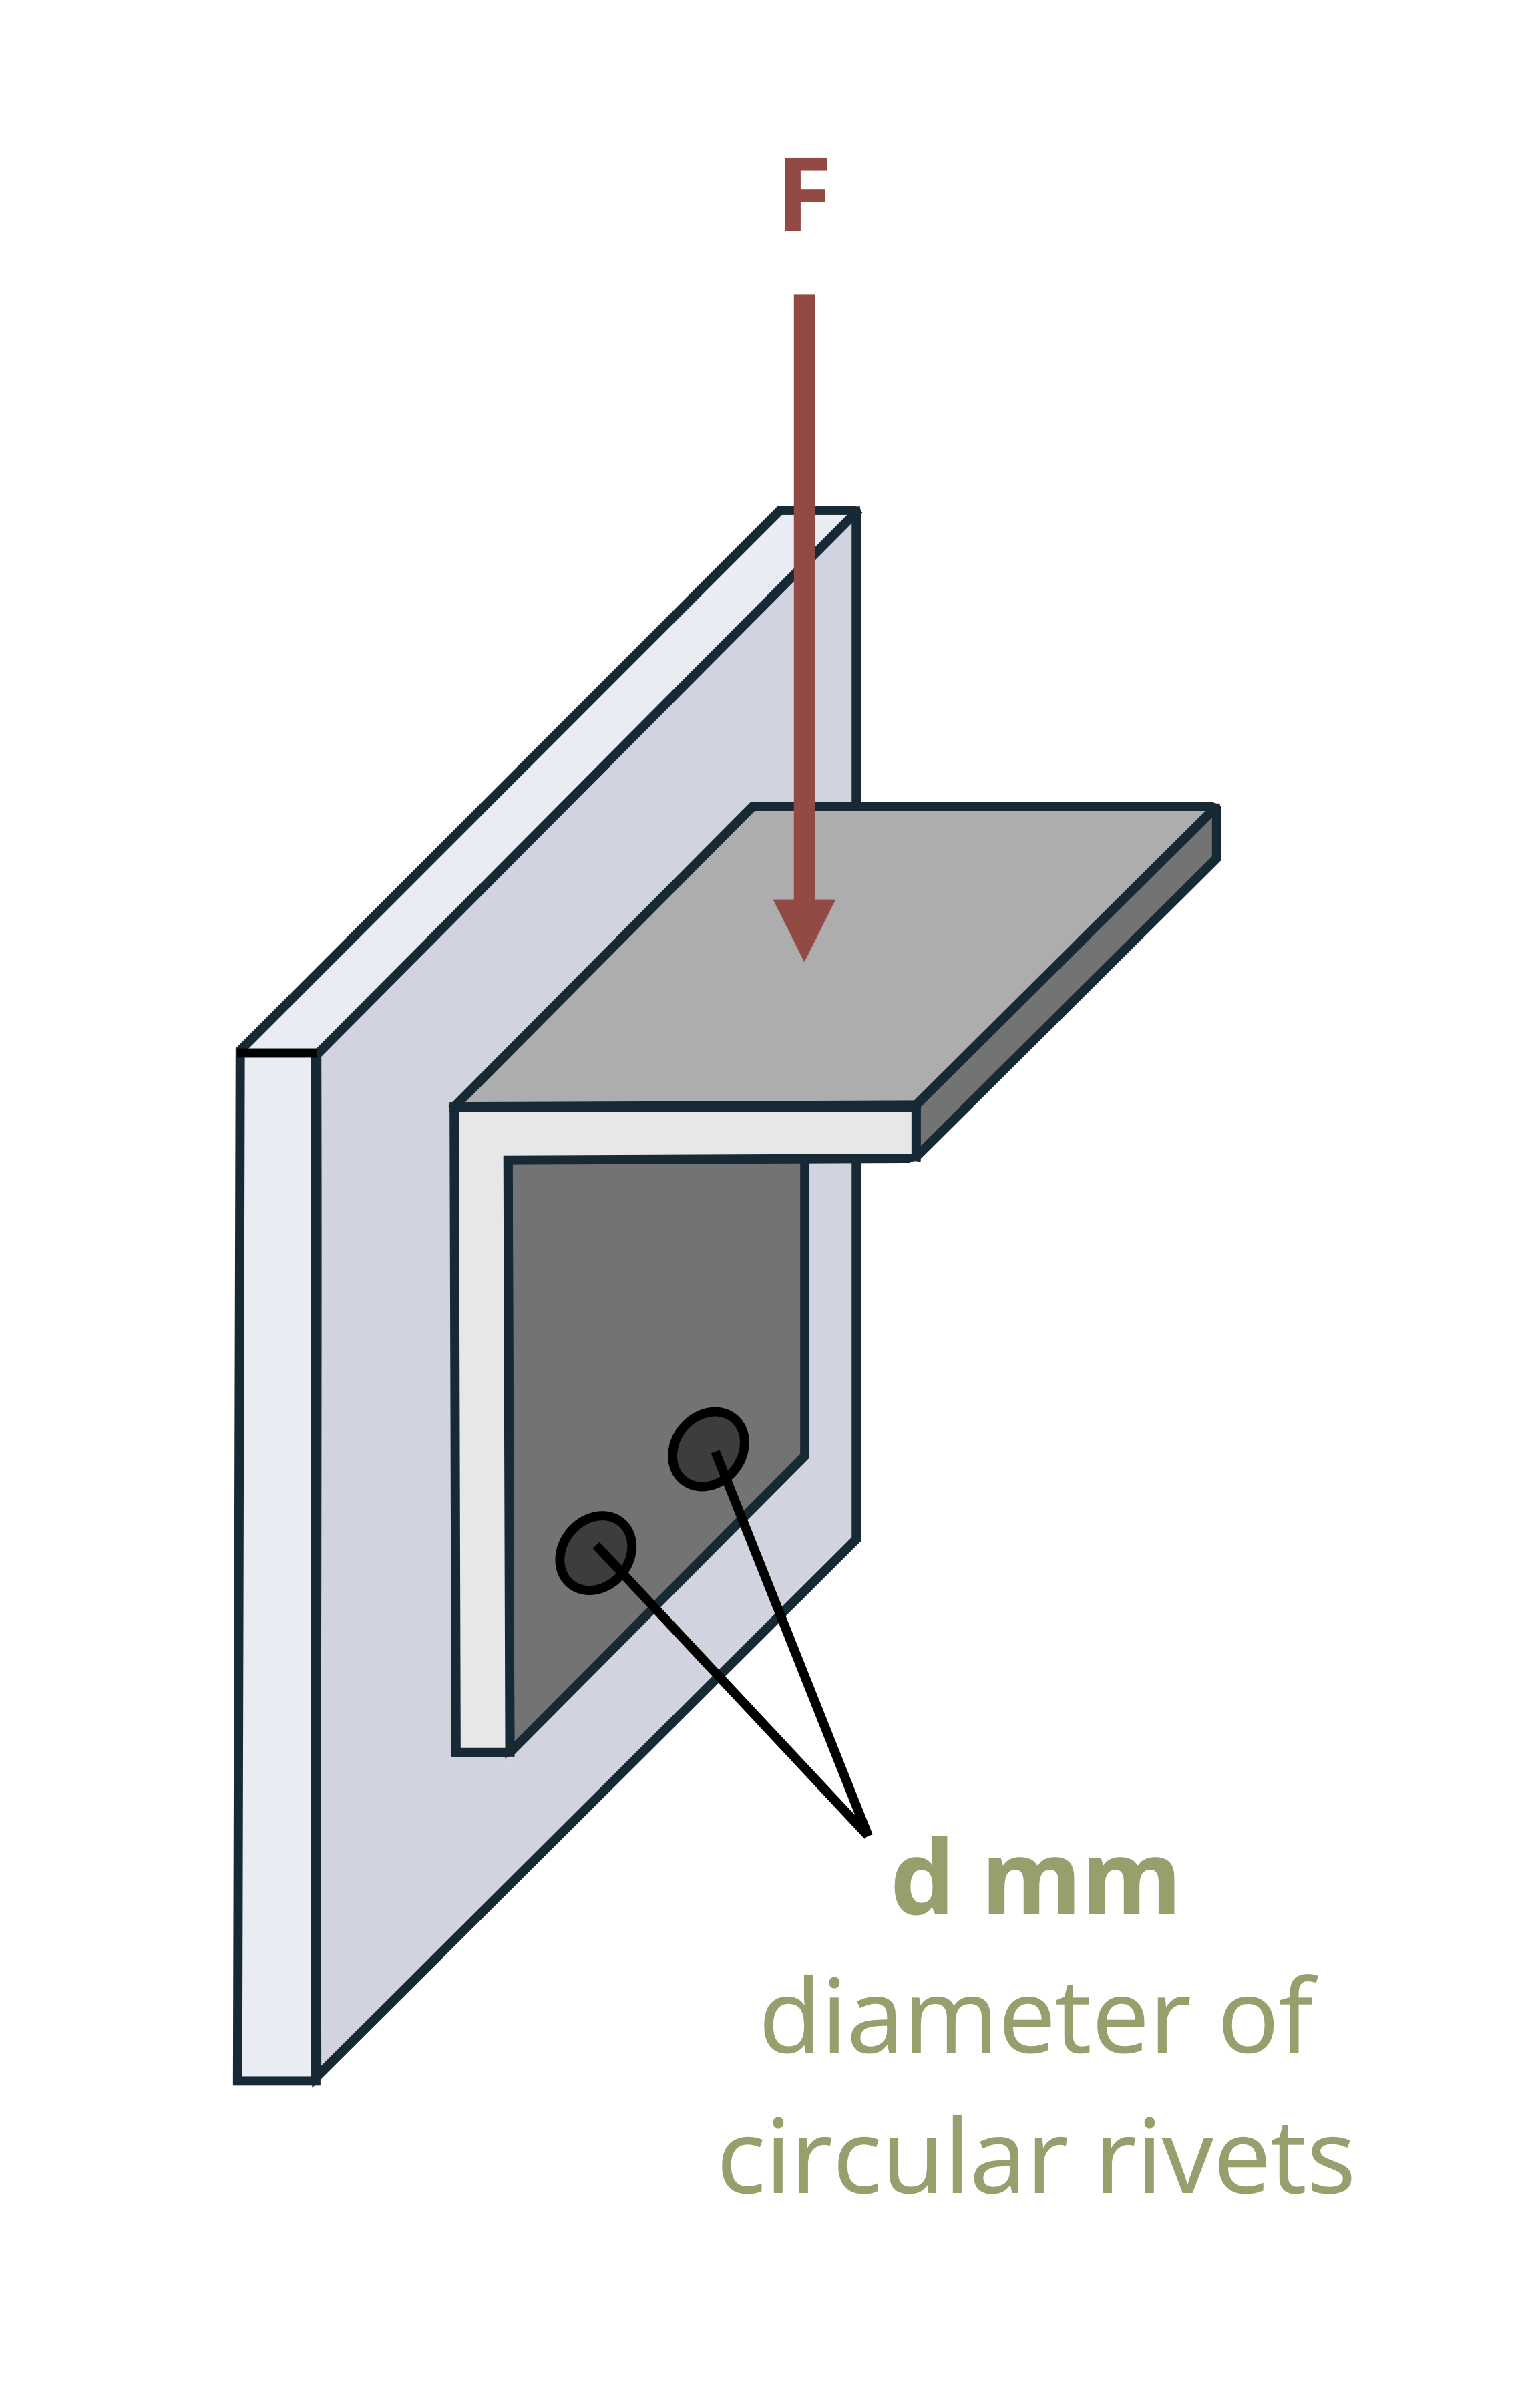
\includegraphics{images/165.png}

}

\caption{Figure 1: A bracket is attached to a wall with two circular
rivets}

\end{figure}%

\begin{Shaded}
\begin{Highlighting}[]
\NormalTok{\#| standalone: true}
\NormalTok{\#| viewerHeight: 600}
\NormalTok{\#| components: [viewer]}

\NormalTok{from shiny import App, render, ui, reactive}
\NormalTok{import random}
\NormalTok{import asyncio}
\NormalTok{import io}
\NormalTok{import math}
\NormalTok{import string}
\NormalTok{from datetime import datetime}
\NormalTok{from pathlib import Path}

\NormalTok{def generate\_random\_letters(length):}
\NormalTok{    \# Generate a random string of letters of specified length}
\NormalTok{    return \textquotesingle{}\textquotesingle{}.join(random.choice(string.ascii\_lowercase) for \_ in range(length))}

\NormalTok{problem\_ID="165"}
\NormalTok{F=reactive.Value("\_\_")}
\NormalTok{d=reactive.Value("\_\_")}


\NormalTok{attempts=["Timestamp,Attempt,Answer,Feedback\textbackslash{}n"]}

\NormalTok{app\_ui = ui.page\_fluid(}
\NormalTok{    ui.markdown("**Please enter your ID number from your instructor and click to generate your problem**"),}
\NormalTok{    ui.input\_text("ID","", placeholder="Enter ID Number Here"),}
\NormalTok{    ui.input\_action\_button("generate\_problem", "Generate Problem", class\_="btn{-}primary"),}
\NormalTok{    ui.markdown("**Problem Statement**"),}
\NormalTok{    ui.output\_ui("ui\_problem\_statement"),}
\NormalTok{    ui.input\_text("answer","Your Answer in units of MPa", placeholder="Please enter your answer"),}
\NormalTok{    ui.input\_action\_button("submit", "Submit Answer", class\_="btn{-}primary"),}
\NormalTok{    ui.download\_button("download", "Download File to Submit", class\_="btn{-}success"),}
\NormalTok{)}


\NormalTok{def server(input, output, session):}
\NormalTok{    \# Initialize a counter for attempts}
\NormalTok{    attempt\_counter = reactive.Value(0)}

\NormalTok{    @output}
\NormalTok{    @render.ui}
\NormalTok{    def ui\_problem\_statement():}
\NormalTok{        return[ui.markdown(f"A bracket is attached to a wall with two circular rivets of diameter d = \{d()\} mm. A load F = \{F()\} kN is applied in the center of the bracket. Assuming the load is split evenly between the two rivits, determine the shear stress in each rivet. ")]}
    
\NormalTok{    @reactive.Effect}
\NormalTok{    @reactive.event(input.generate\_problem)}
\NormalTok{    def randomize\_vars():}
\NormalTok{        random.seed(input.ID())}
\NormalTok{        F.set(random.randrange(30, 100, 1))}
\NormalTok{        d.set(random.randrange(10, 40, 1))}
        

\NormalTok{    @reactive.Effect}
\NormalTok{    @reactive.event(input.submit)}
\NormalTok{    def \_():}
\NormalTok{        attempt\_counter.set(attempt\_counter() + 1)  \# Increment the attempt counter on each submission.  }
      
\NormalTok{        A = math.pi*(d()/(1000*2))**2}
\NormalTok{        instr= ((F()/2)/A)/1000}
\NormalTok{        if math.isclose(float(input.answer()), instr, rel\_tol=0.001):}
\NormalTok{            check = "*Correct*"}
\NormalTok{            correct\_indicator = "JL"}
\NormalTok{        else:}
\NormalTok{            check = "*Not Correct.*"}
\NormalTok{            correct\_indicator = "JG"}

\NormalTok{        \# Generate random parts for the encoded attempt.}
\NormalTok{        random\_start = generate\_random\_letters(4)}
\NormalTok{        random\_middle = generate\_random\_letters(4)}
\NormalTok{        random\_end = generate\_random\_letters(4)}
\NormalTok{        encoded\_attempt = f"\{random\_start\}\{problem\_ID\}{-}\{random\_middle\}\{attempt\_counter()\}\{correct\_indicator\}{-}\{random\_end\}\{input.ID()\}"}

\NormalTok{        \# Store the most recent encoded attempt in a reactive value so it persists across submissions}
\NormalTok{        session.encoded\_attempt = reactive.Value(encoded\_attempt)}

\NormalTok{        \# Append the attempt data to the attempts list without the encoded attempt}
\NormalTok{        attempts.append(f"\{datetime.now()\}, \{attempt\_counter()\}, \{input.answer()\}, \{check\}\textbackslash{}n")}

\NormalTok{        \# Show feedback to the user.}
\NormalTok{        feedback = ui.markdown(f"Your answer of \{input.answer()\} is \{check\}. For reference in debugging this, the calculated instructor answer is \{instr\}")}
\NormalTok{        m = ui.modal(}
\NormalTok{            feedback,}
\NormalTok{            title="Feedback",}
\NormalTok{            easy\_close=True}
\NormalTok{        )}
\NormalTok{        ui.modal\_show(m)}

\NormalTok{    @session.download(filename=lambda: f"Problem\_Log{-}\{problem\_ID\}{-}\{input.ID()\}.csv")}
\NormalTok{    async def download():}
\NormalTok{        \# Start the CSV with the encoded attempt (without label)}
\NormalTok{        final\_encoded = session.encoded\_attempt() if session.encoded\_attempt is not None else "No attempts"}
\NormalTok{        yield f"\{final\_encoded\}\textbackslash{}n\textbackslash{}n"}
        
\NormalTok{        \# Write the header for the remaining CSV data once}
\NormalTok{        yield "Timestamp,Attempt,Answer,Feedback\textbackslash{}n"}
        
\NormalTok{        \# Write the attempts data, ensure that the header from the attempts list is not written again}
\NormalTok{        for attempt in attempts[1:]:  \# Skip the first element which is the header}
\NormalTok{            await asyncio.sleep(0.25)  \# This delay may not be necessary; adjust as needed}
\NormalTok{            yield attempt}


\NormalTok{\# App installation}
\NormalTok{app = App(app\_ui, server)}
\end{Highlighting}
\end{Shaded}

\chapter*{Problem 2.37}\label{problem-2.37}
\addcontentsline{toc}{chapter}{Problem 2.37}

\markboth{Problem 2.37}{Problem 2.37}

This is a dynamic rendering of the problem with dynamic variables based
on the username entered.

\section*{Problem Image}\label{problem-image-10}
\addcontentsline{toc}{section}{Problem Image}

\markright{Problem Image}

\begin{figure}[H]

{\centering 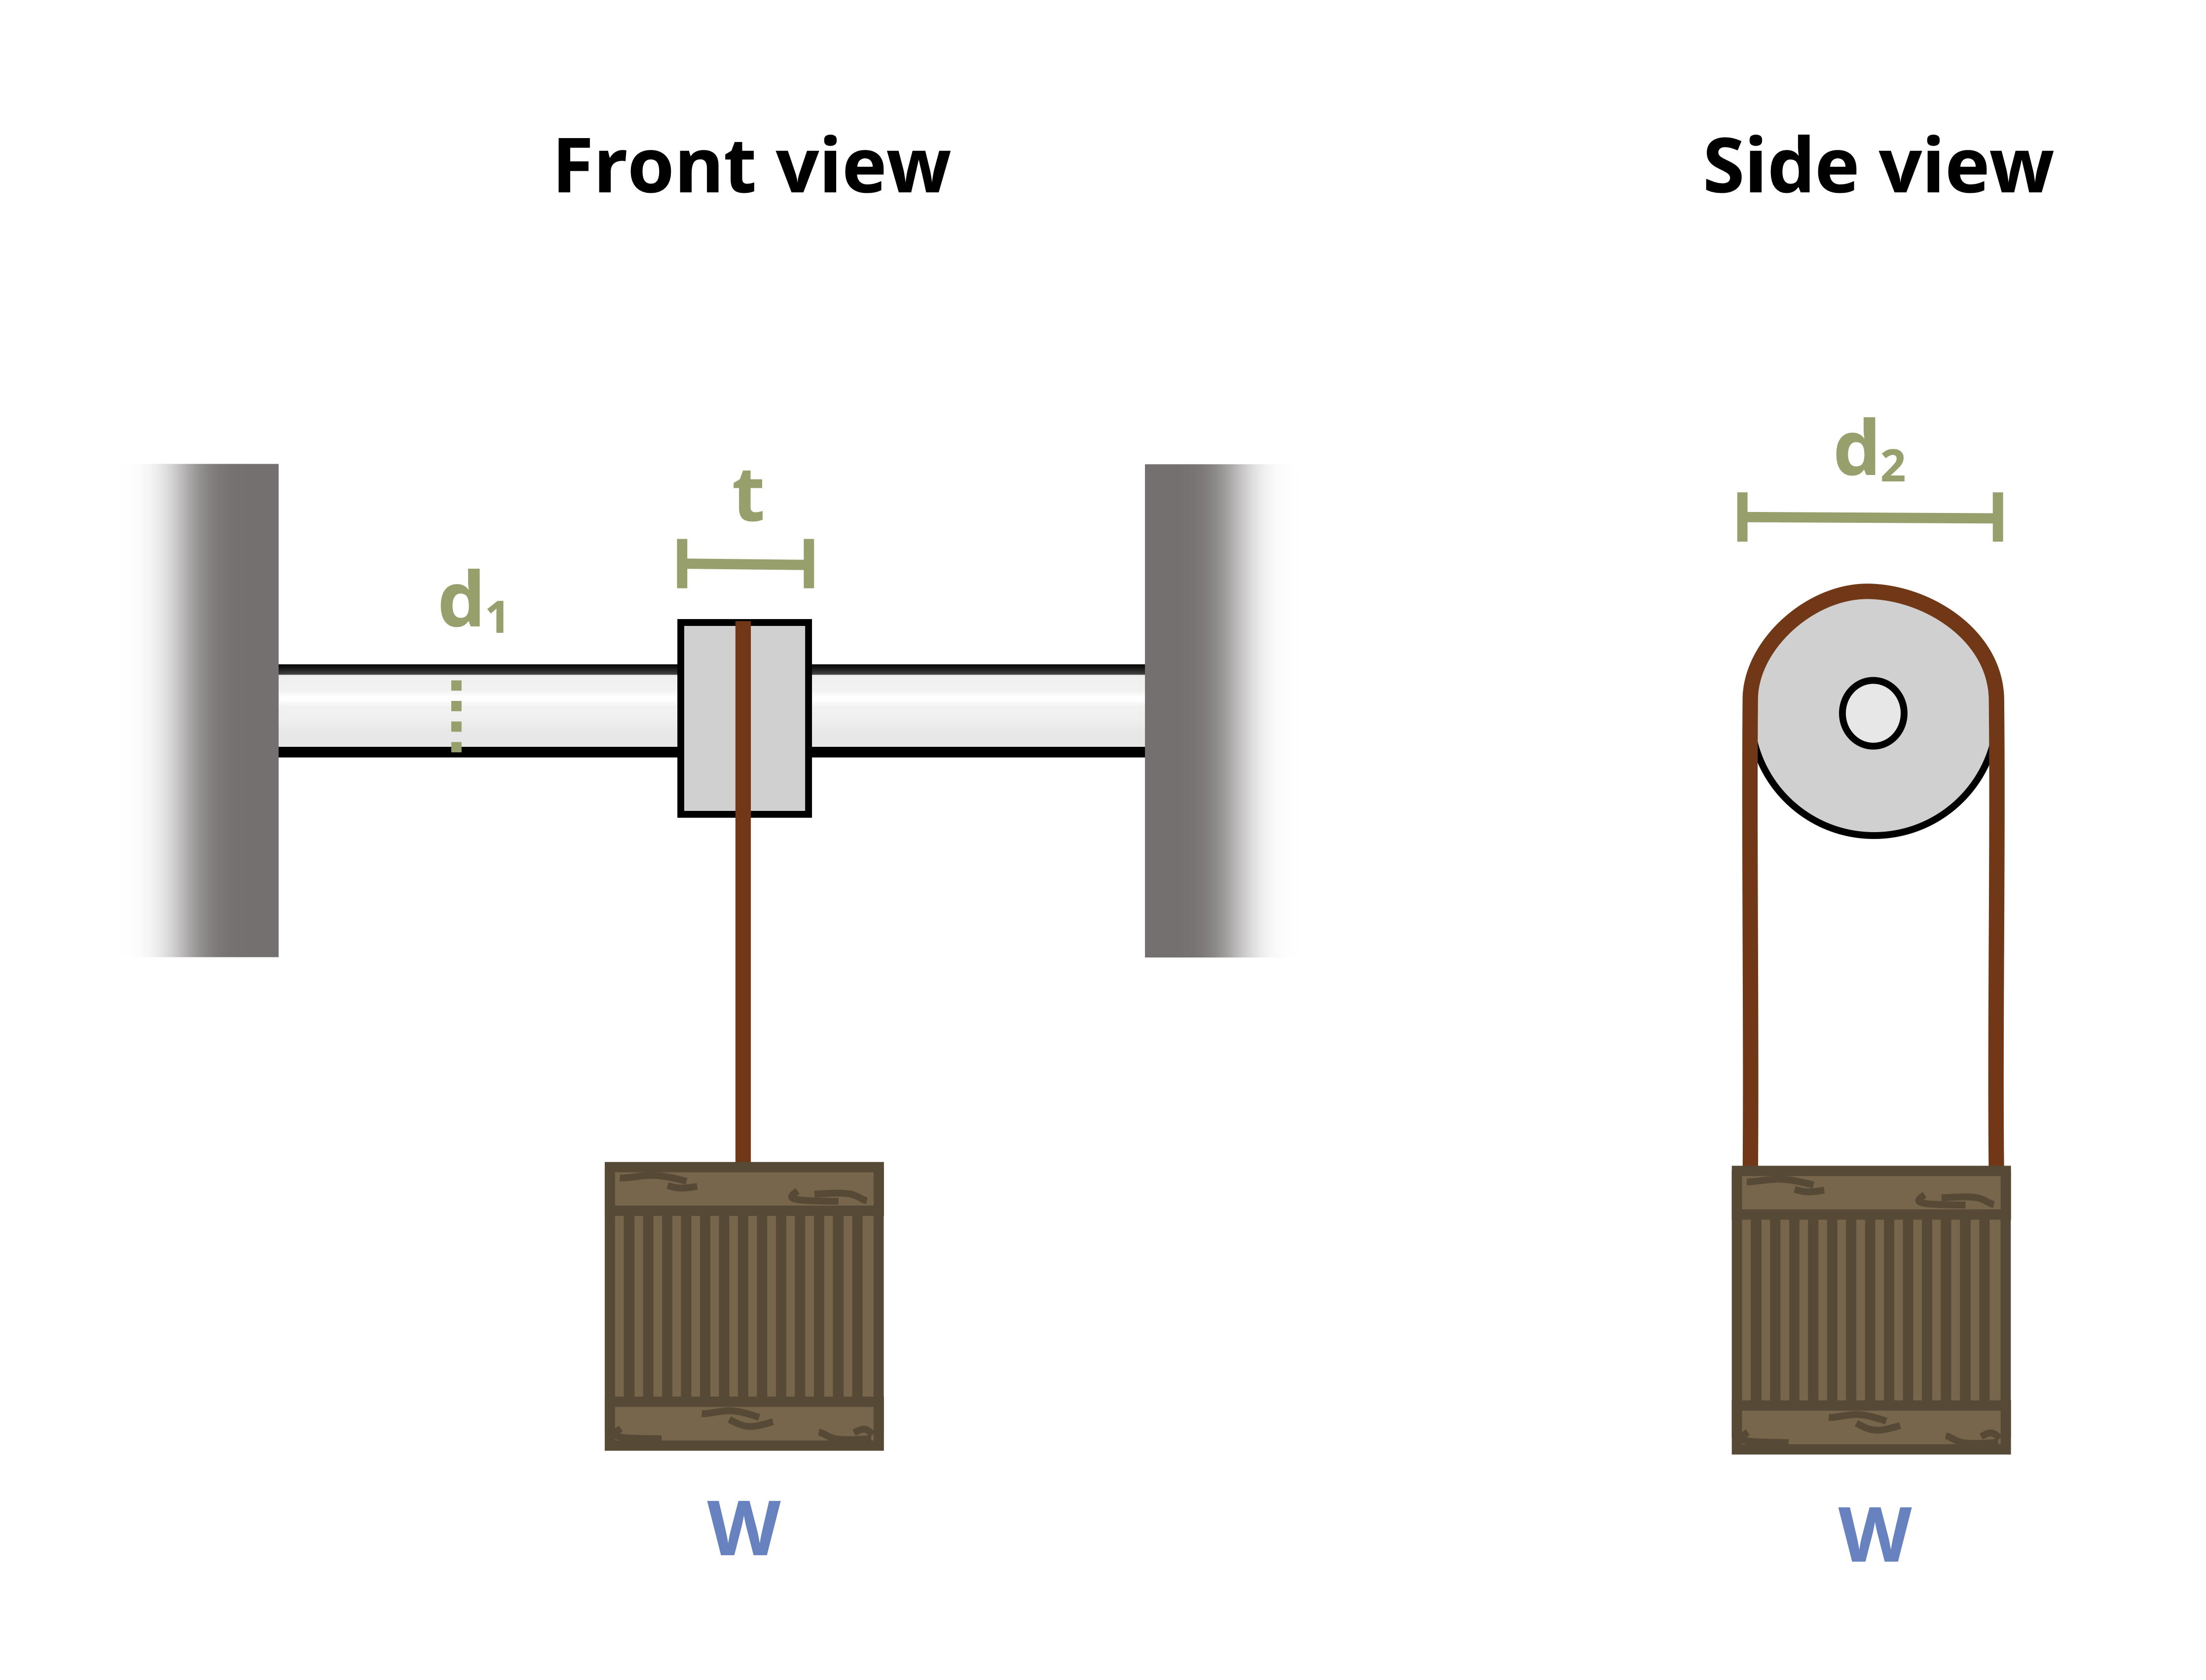
\includegraphics{images/166.png}

}

\caption{Figure 1: A crate is hanged on a circular solid metal rod.}

\end{figure}%

\begin{Shaded}
\begin{Highlighting}[]
\NormalTok{\#| standalone: true}
\NormalTok{\#| viewerHeight: 600}
\NormalTok{\#| components: [viewer]}

\NormalTok{from shiny import App, render, ui, reactive}
\NormalTok{import random}
\NormalTok{import asyncio}
\NormalTok{import io}
\NormalTok{import math}
\NormalTok{import string}
\NormalTok{from datetime import datetime}
\NormalTok{from pathlib import Path}

\NormalTok{problem\_ID="166"}
\NormalTok{W=reactive.Value("\_\_")}
\NormalTok{d1=reactive.Value("\_\_")}
\NormalTok{d2=reactive.Value("\_\_")}
\NormalTok{t=reactive.Value("\_\_")}

\NormalTok{def generate\_random\_letters(length):}
\NormalTok{    \# Generate a random string of letters of specified length}
\NormalTok{    return \textquotesingle{}\textquotesingle{}.join(random.choice(string.ascii\_lowercase) for \_ in range(length)) }

\NormalTok{attempts=["Timestamp,Attempt,Answer,Feedback\textbackslash{}n"]}

\NormalTok{app\_ui = ui.page\_fluid(}
\NormalTok{    ui.markdown("**Please enter your ID number from your instructor and click to generate your problem**"),}
\NormalTok{    ui.input\_text("ID","", placeholder="Enter ID Number Here"),}
\NormalTok{    ui.input\_action\_button("generate\_problem", "Generate Problem", class\_="btn{-}primary"),}
\NormalTok{    ui.markdown("**Problem Statement**"),}
\NormalTok{    ui.output\_ui("ui\_problem\_statement"),}
\NormalTok{    ui.input\_text("answer","Your Answer in units of ksi", placeholder="Please enter your answer"),}
\NormalTok{    ui.input\_action\_button("submit", "Submit Answer", class\_="btn{-}primary"),}
\NormalTok{    ui.download\_button("download", "Download File to Submit", class\_="btn{-}success"),}
\NormalTok{)}


\NormalTok{def server(input, output, session):}
\NormalTok{    \# Initialize a counter for attempts}
\NormalTok{    attempt\_counter = reactive.Value(0)}

\NormalTok{    @output}
\NormalTok{    @render.ui}
\NormalTok{    def ui\_problem\_statement():}
\NormalTok{        return[ui.markdown(f"A crate of weight W = \{W()\} lb hangs from a solid circular metal rod of diameter d\textless{}sub\textgreater{}1\textless{}/sub\textgreater{} = \{d1()\} in.. The cable is wrapped around a support collar of diameter d\textless{}sub\textgreater{}2\textless{}/sub\textgreater{} = \{d2()\} in. and thickness t = \{t()\} in. to evenly distribute the cable load. What is the bearing stress on the support collar due to the rod? ")]}
    
\NormalTok{    @reactive.Effect}
\NormalTok{    @reactive.event(input.generate\_problem)}
\NormalTok{    def randomize\_vars():}
\NormalTok{        random.seed(input.ID())}
\NormalTok{        W.set(random.randrange(4000, 9000, 100))}
\NormalTok{        d1.set(random.randrange(5, 30, 1)/10)}
\NormalTok{        d2.set(round(d1() * 3, 2))}
\NormalTok{        t.set(round(d1() * 2, 2))}

\NormalTok{    @reactive.Effect}
\NormalTok{    @reactive.event(input.submit)}
\NormalTok{    def \_():}
\NormalTok{        attempt\_counter.set(attempt\_counter() + 1)  \# Increment the attempt counter on each submission.}
    
\NormalTok{        instr= (W()/(d1()*t()))/1000}
\NormalTok{        if math.isclose(float(input.answer()), instr, rel\_tol=0.001):}
\NormalTok{            check = "*Correct*"}
\NormalTok{            correct\_indicator = "JL"}
\NormalTok{        else:}
\NormalTok{            check = "*Not Correct.*"}
\NormalTok{            correct\_indicator = "JG"}

\NormalTok{        \# Generate random parts for the encoded attempt.}
\NormalTok{        random\_start = generate\_random\_letters(4)}
\NormalTok{        random\_middle = generate\_random\_letters(4)}
\NormalTok{        random\_end = generate\_random\_letters(4)}
\NormalTok{        encoded\_attempt = f"\{random\_start\}\{problem\_ID\}{-}\{random\_middle\}\{attempt\_counter()\}\{correct\_indicator\}{-}\{random\_end\}\{input.ID()\}"}

\NormalTok{        \# Store the most recent encoded attempt in a reactive value so it persists across submissions}
\NormalTok{        session.encoded\_attempt = reactive.Value(encoded\_attempt)}

\NormalTok{        \# Append the attempt data to the attempts list without the encoded attempt}
\NormalTok{        attempts.append(f"\{datetime.now()\}, \{attempt\_counter()\}, \{input.answer()\}, \{check\}\textbackslash{}n")}

\NormalTok{        \# Show feedback to the user.}
\NormalTok{        feedback = ui.markdown(f"Your answer of \{input.answer()\} is \{check\}. For reference in debugging this, the calculated instructor answer is \{instr\}")}
\NormalTok{        m = ui.modal(}
\NormalTok{            feedback,}
\NormalTok{            title="Feedback",}
\NormalTok{            easy\_close=True}
\NormalTok{        )}
\NormalTok{        ui.modal\_show(m)}

\NormalTok{    @session.download(filename=lambda: f"Problem\_Log{-}\{problem\_ID\}{-}\{input.ID()\}.csv")}
\NormalTok{    async def download():}
\NormalTok{        \# Start the CSV with the encoded attempt (without label)}
\NormalTok{        final\_encoded = session.encoded\_attempt() if session.encoded\_attempt is not None else "No attempts"}
\NormalTok{        yield f"\{final\_encoded\}\textbackslash{}n\textbackslash{}n"}
        
\NormalTok{        \# Write the header for the remaining CSV data once}
\NormalTok{        yield "Timestamp,Attempt,Answer,Feedback\textbackslash{}n"}
        
\NormalTok{        \# Write the attempts data, ensure that the header from the attempts list is not written again}
\NormalTok{        for attempt in attempts[1:]:  \# Skip the first element which is the header}
\NormalTok{            await asyncio.sleep(0.25)  \# This delay may not be necessary; adjust as needed}
\NormalTok{            yield attempt}


\NormalTok{\# App installation}
\NormalTok{app = App(app\_ui, server)}
\end{Highlighting}
\end{Shaded}

\chapter*{Problem 2.40}\label{problem-2.40}
\addcontentsline{toc}{chapter}{Problem 2.40}

\markboth{Problem 2.40}{Problem 2.40}

This is a dynamic rendering of the problem with dynamic variables based
on the username entered.

\section*{Problem Image}\label{problem-image-11}
\addcontentsline{toc}{section}{Problem Image}

\markright{Problem Image}

\begin{figure}[H]

{\centering 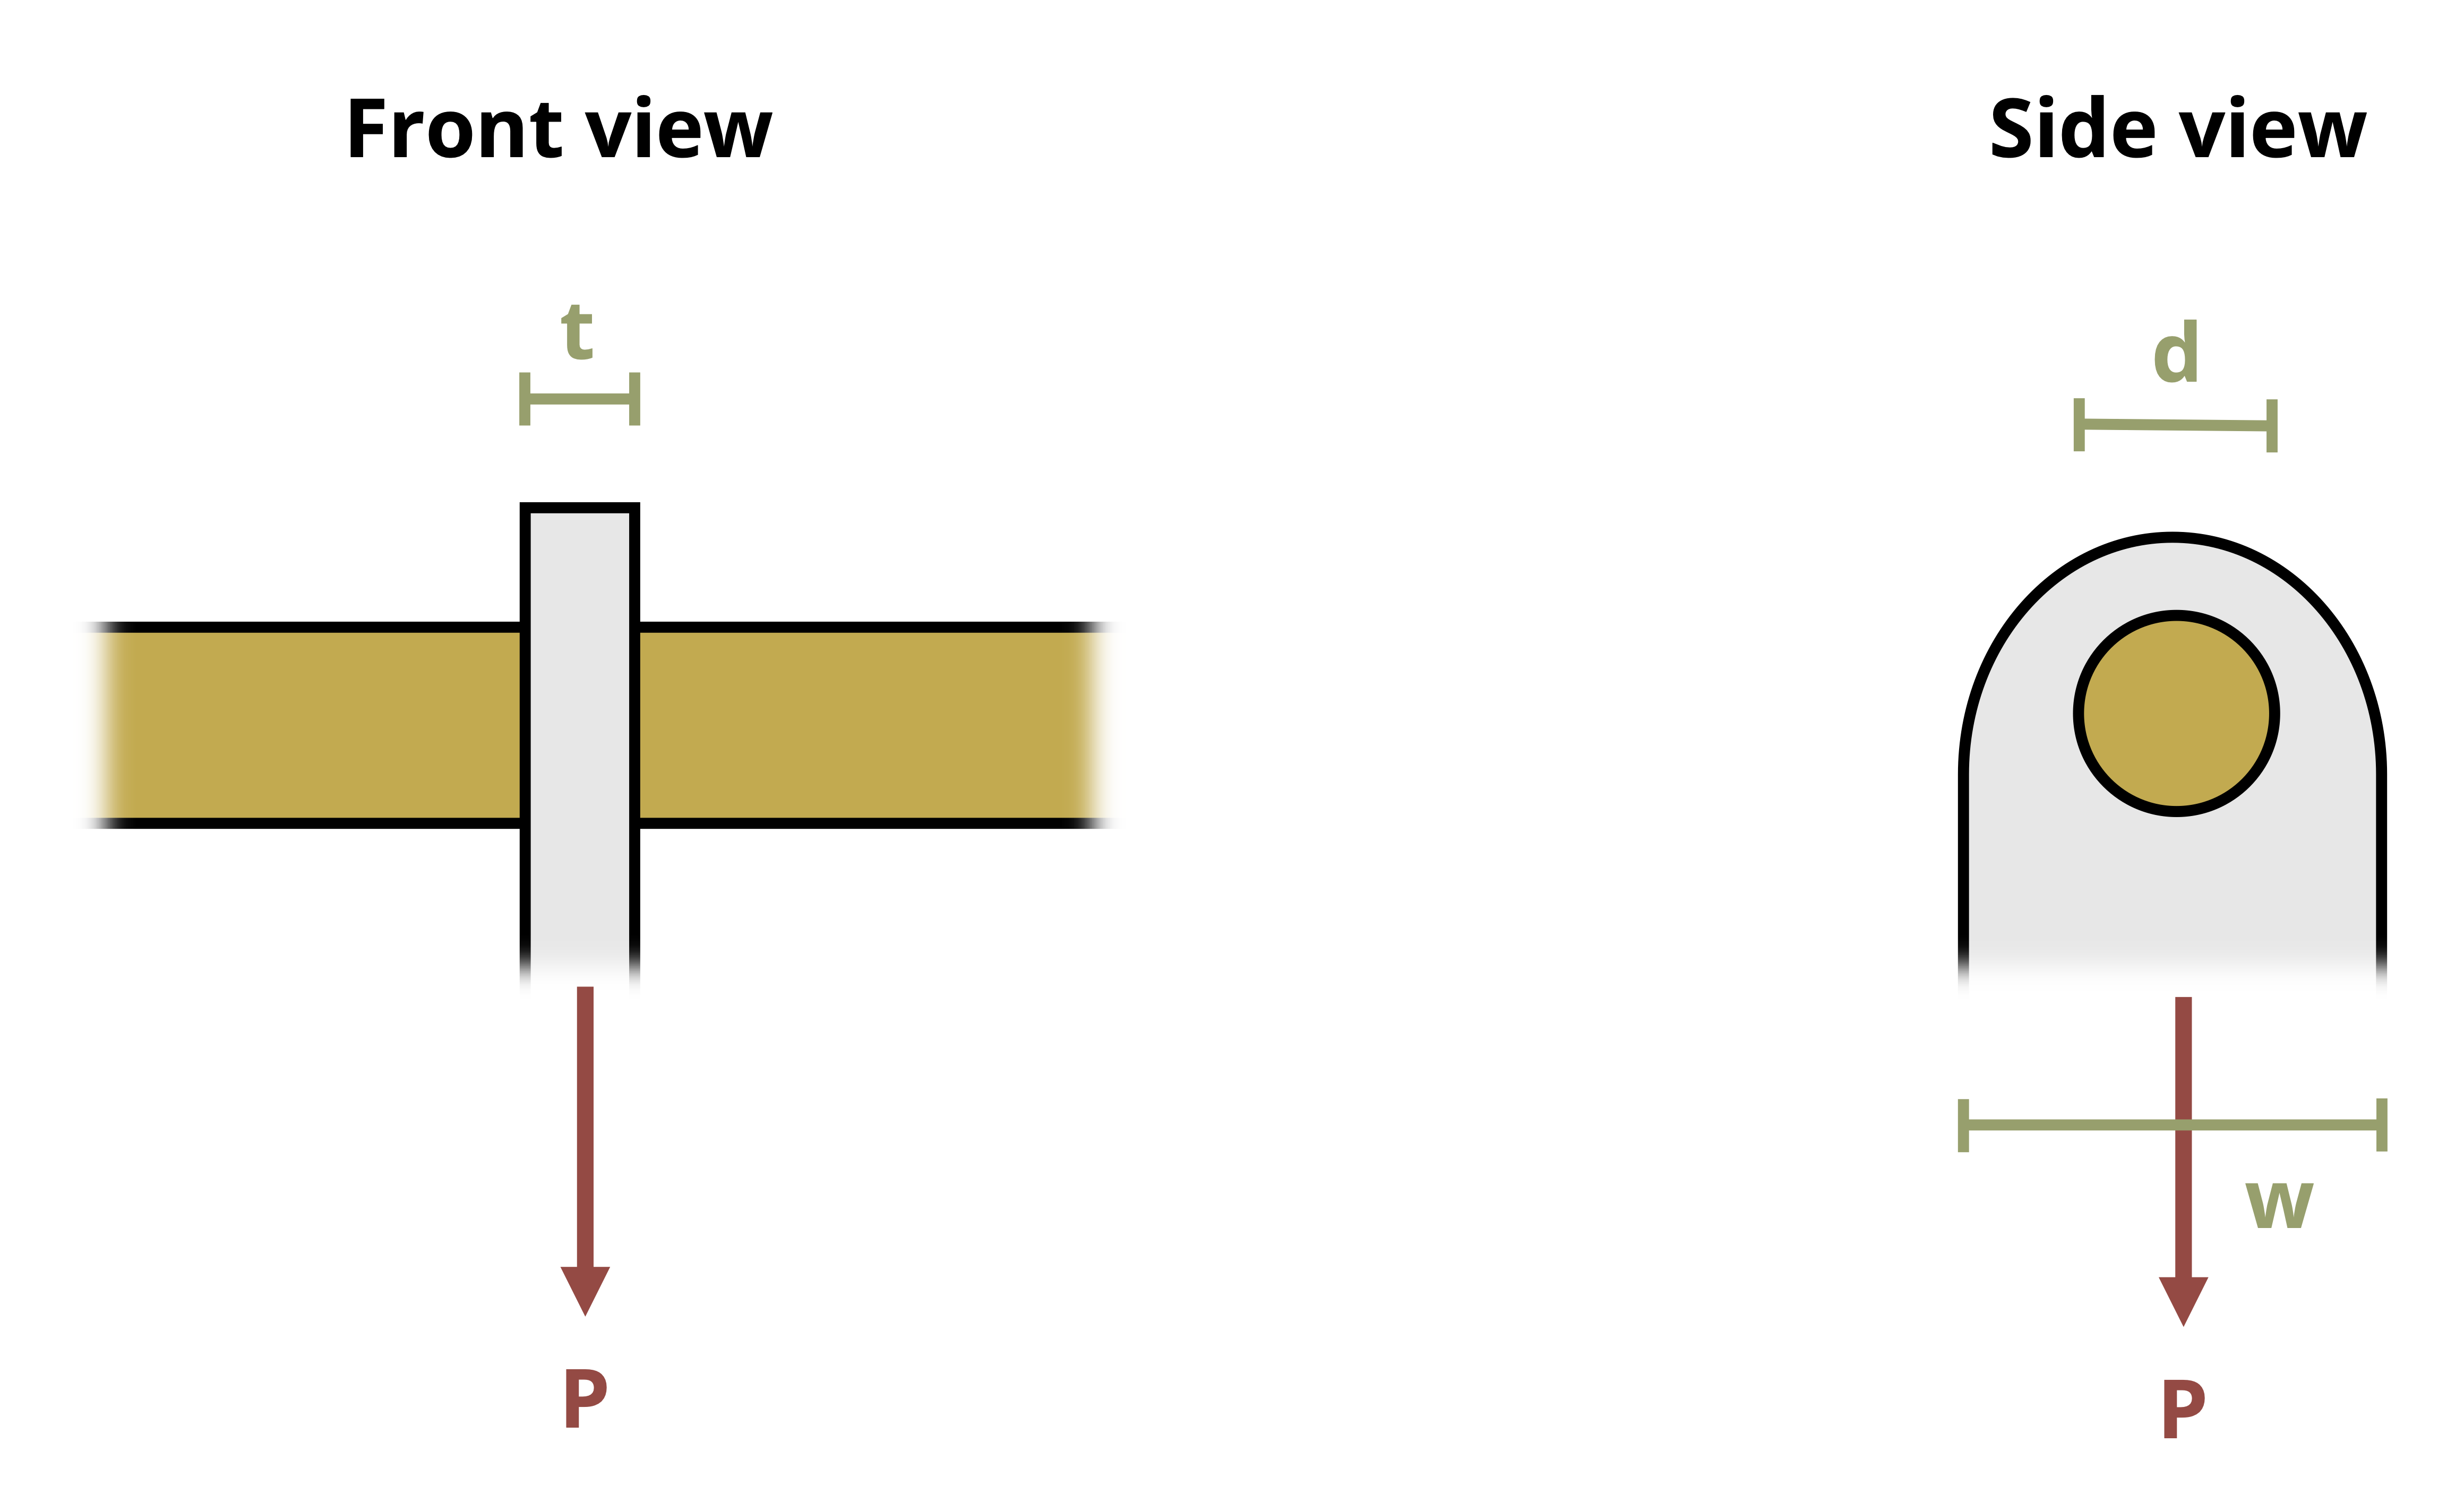
\includegraphics{images/169.png}

}

\caption{Figure 1: A steel connector plate is hung from a brass rod.}

\end{figure}%

\begin{Shaded}
\begin{Highlighting}[]
\NormalTok{\#| standalone: true}
\NormalTok{\#| viewerHeight: 600}
\NormalTok{\#| components: [viewer]}

\NormalTok{from shiny import App, render, ui, reactive}
\NormalTok{import random}
\NormalTok{import asyncio}
\NormalTok{import io}
\NormalTok{import math}
\NormalTok{import string}
\NormalTok{from datetime import datetime}
\NormalTok{from pathlib import Path}

\NormalTok{def generate\_random\_letters(length):}
\NormalTok{    \# Generate a random string of letters of specified length}
\NormalTok{    return \textquotesingle{}\textquotesingle{}.join(random.choice(string.ascii\_lowercase) for \_ in range(length))}

\NormalTok{problem\_ID="169"}
\NormalTok{d=reactive.Value("\_\_")}
\NormalTok{t=reactive.Value("\_\_")}
\NormalTok{w=reactive.Value("\_\_")}
\NormalTok{Fbrass = 70}
\NormalTok{Fsteel = 75}


\NormalTok{attempts=["Timestamp,Attempt,Answer,Feedback\textbackslash{}n"]}

\NormalTok{app\_ui = ui.page\_fluid(}
\NormalTok{    ui.markdown("**Please enter your ID number from your instructor and click to generate your problem**"),}
\NormalTok{    ui.input\_text("ID","", placeholder="Enter ID Number Here"),}
\NormalTok{    ui.input\_action\_button("generate\_problem", "Generate Problem", class\_="btn{-}primary"),}
\NormalTok{    ui.markdown("**Problem Statement**"),}
\NormalTok{    ui.output\_ui("ui\_problem\_statement"),}
\NormalTok{    ui.input\_text("answer","Your Answer in units of kips", placeholder="Please enter your answer"),}
\NormalTok{    ui.input\_action\_button("submit", "Submit Answer", class\_="btn{-}primary"),}
\NormalTok{    ui.download\_button("download", "Download File to Submit", class\_="btn{-}success"),}
\NormalTok{)}


\NormalTok{def server(input, output, session):}
\NormalTok{    \# Initialize a counter for attempts}
\NormalTok{    attempt\_counter = reactive.Value(0)}

\NormalTok{    @output}
\NormalTok{    @render.ui}
\NormalTok{    def ui\_problem\_statement():}
\NormalTok{        return[ui.markdown(f"A steel connector plate is hung from a brass rod of diameter d = \{d()\} in. The plate has dimensions t = \{t()\} in. and w = \{w()\} in. Find the minimum load that will cause the connector or rod to fail. Assume the tensile and compressive failure stress for brass is 70 ksi and for steel is 75 ksi. Assume the shear failure stress for each material is one half of the tensile{-}compressive failure stress. ")]}
    
\NormalTok{    @reactive.Effect}
\NormalTok{    @reactive.event(input.generate\_problem)}
\NormalTok{    def randomize\_vars():}
\NormalTok{        random.seed(input.ID())}
\NormalTok{        d.set(random.randrange(8, 20, 1)/10)}
\NormalTok{        t.set(random.randrange(3, 7, 1)/10)}
\NormalTok{        w.set(round(d() * 2, 2))}
        

\NormalTok{    @reactive.Effect}
\NormalTok{    @reactive.event(input.submit)}
\NormalTok{    def \_():}
\NormalTok{        attempt\_counter.set(attempt\_counter() + 1)  \# Increment the attempt counter on each submission.  }
      
\NormalTok{        instr= (Fsteel/2)*(2*.866*(w(){-}d())/2)}
\NormalTok{        if math.isclose(float(input.answer()), instr, rel\_tol=0.001):}
\NormalTok{            check = "*Correct*"}
\NormalTok{            correct\_indicator = "JL"}
\NormalTok{        else:}
\NormalTok{            check = "*Not Correct.*"}
\NormalTok{            correct\_indicator = "JG"}

\NormalTok{        \# Generate random parts for the encoded attempt.}
\NormalTok{        random\_start = generate\_random\_letters(4)}
\NormalTok{        random\_middle = generate\_random\_letters(4)}
\NormalTok{        random\_end = generate\_random\_letters(4)}
\NormalTok{        encoded\_attempt = f"\{random\_start\}\{problem\_ID\}{-}\{random\_middle\}\{attempt\_counter()\}\{correct\_indicator\}{-}\{random\_end\}\{input.ID()\}"}

\NormalTok{        \# Store the most recent encoded attempt in a reactive value so it persists across submissions}
\NormalTok{        session.encoded\_attempt = reactive.Value(encoded\_attempt)}

\NormalTok{        \# Append the attempt data to the attempts list without the encoded attempt}
\NormalTok{        attempts.append(f"\{datetime.now()\}, \{attempt\_counter()\}, \{input.answer()\}, \{check\}\textbackslash{}n")}

\NormalTok{        \# Show feedback to the user.}
\NormalTok{        feedback = ui.markdown(f"Your answer of \{input.answer()\} is \{check\}. For reference in debugging this, the calculated instructor answer is \{instr\}")}
\NormalTok{        m = ui.modal(}
\NormalTok{            feedback,}
\NormalTok{            title="Feedback",}
\NormalTok{            easy\_close=True}
\NormalTok{        )}
\NormalTok{        ui.modal\_show(m)}

\NormalTok{    @session.download(filename=lambda: f"Problem\_Log{-}\{problem\_ID\}{-}\{input.ID()\}.csv")}
\NormalTok{    async def download():}
\NormalTok{        \# Start the CSV with the encoded attempt (without label)}
\NormalTok{        final\_encoded = session.encoded\_attempt() if session.encoded\_attempt is not None else "No attempts"}
\NormalTok{        yield f"\{final\_encoded\}\textbackslash{}n\textbackslash{}n"}
        
\NormalTok{        \# Write the header for the remaining CSV data once}
\NormalTok{        yield "Timestamp,Attempt,Answer,Feedback\textbackslash{}n"}
        
\NormalTok{        \# Write the attempts data, ensure that the header from the attempts list is not written again}
\NormalTok{        for attempt in attempts[1:]:  \# Skip the first element which is the header}
\NormalTok{            await asyncio.sleep(0.25)  \# This delay may not be necessary; adjust as needed}
\NormalTok{            yield attempt}


\NormalTok{\# App installation}
\NormalTok{app = App(app\_ui, server)}
\end{Highlighting}
\end{Shaded}

\bookmarksetup{startatroot}

\chapter{Summary}\label{summary}

In summary, this book has no content whatsoever.

\bookmarksetup{startatroot}

\chapter*{References}\label{references}
\addcontentsline{toc}{chapter}{References}

\markboth{References}{References}

\phantomsection\label{refs}
\begin{CSLReferences}{0}{1}
\end{CSLReferences}



\end{document}
